 \documentclass[a4paper,14pt]{report} %размер бумаги устанавливаем А4, шрифт 14пунктов
 \usepackage{kmanual} %собственный стиль

 %\includeonly{Title_ug, intr_ug, gen_ug}
 \makeatletter

 \makeatother

 % колонтитулы:
 \pagestyle{fancy}
  \fancyhead{} %очистим хидер на всякий случай
  \fancyfoot{} %очистим футер 
  \renewcommand{\sectionmark}[1]{\protect\markright{\textit{#1}}}
  \fancyfoot[R]{\thepage} %номер страницы справа внизу
  \fancyhead[R]{\parbox[b]{300pt}{\flushright{\textbf{\textit{\\ МИС Амбулатория}}}}}
  \fancyhead[L]{
\includegraphics[width = 100pt, keepaspectratio]{logo}}
  \fancyfoot[L]{\textit{Руководство пользователя} \\ \rightmark} 
  \renewcommand{\headrulewidth}{0.3pt}
  \renewcommand{\footrulewidth}{0.3pt}
  \addtolength{\headheight}{0.3pt} % оставляем место для линейки
 \fancypagestyle{plain}

 \fancypagestyle{firststyle} %стиль первой страницы
 {
  \fancyhead{} %очистим хидер на всякий случай
  \fancyfoot{} %очистим футер 
  \fancyhead[R]{\parbox[b]{300pt}{\flushright{\textbf{\textit{\\ МИС Амбулатория}}}}}
  \fancyhead[L]{
\includegraphics[width = 100pt, keepaspectratio]{logo}}
  \renewcommand{\headrulewidth}{0.3pt}
  \renewcommand{\footrulewidth}{0pt}
  \addtolength{\headheight}{0.3pt} % оставляем место для линейки
 }

 \newcommand{\tmis}{МИС Амбулатория}
      
 \begin{document}
   
   \begin{titlepage}
    \newpage
    \thispagestyle{firststyle} %стиль колонтитулов
    
    \begin{center}
    \vspace*{\fill}
    \hbox{%
    \vrule width 4pt\hspace{2em}\parbox{1\textwidth}%
    {\vspace*{0.5em}\raggedright{\Large{\textbf{МЕДИЦИНСКАЯ ИНФОРМАЦИОННАЯ СИСТЕМА АМБУЛАТОРИЯ}}}

    \vspace*{1em}
    \Large{\textbf{РУКОВОДСТВО ПОЛЬЗОВАТЕЛЯ}}
    
    \vspace*{0.5em}
    \ifthenelse{\isnamedefined{regversion}}
    {\regversion}{}
    \ifthenelse{\isnamedefined{doctorversion}}
    {\doctorversion}{}
    \ifthenelse{\isnamedefined{diagnversion}}
    {\diagnversion}{}
    \ifthenelse{\isnamedefined{assistversion}}
    {\assistversion}{}
    }}
  
    \end{center}

    \vspace{\fill}

    \begin{flushleft}
    Дата создания:  15.07.14 \\
 %   \vspace{1em}
    Последнее обновление:  20.04.15\\
 %   \vspace{1em}
    Версия:  1.2\\
    \end{flushleft}
    \clearpage
    \end{titlepage}%титульный лист
  \tableofcontents % оглавление, которое генерируется автоматически
  \newpage
\sect{Введение}

 Настоящий документ предназначен для руководителей, врачей, среднего медицинского персонала медицинского учреждения, работников отделов медицинской статистики, отделов информатизации и автоматизации. 
 
 Данное руководство пользователя содержит все необходимые сведения для организации работы персонала различных уровней в Медицинской информационной системе (\tmis) и предназначено для самостоятельного освоения пользователями всех необходимых операций в соответствии с их ролями и полномочиями в системе, закрепления и расширения ранее полученных знаний и навыков.

 Для работы в \tmis~и понимания материала настоящего документа сотрудник должен владеть основной терминологией пользователя ПК, иметь навыки работы на компьютере не ниже уровня пользователя ПК.

 \tmis~ --- это информационная система персонифицированного учета оказания медицинской помощи на уровне медицинского учреждения и региона или страны в целом, разработанная с учетом реализации требований по защите персональных данных.

 Внедрение \tmis~ преследует следующие цели:
\begin{itemize}
 	\item повышение качества лечебно-диагностического процесса;
 	\item снижение нагрузки на медицинский персонал;
 	\item контроль обоснованности расходов на оказание медицинской помощи;
 	\item оперативный доступ к медицинской информации и статистическим данным ЛПУ для принятия управленческих решений.
\end{itemize}

 \tmis~ автоматизирует работу медицинского учреждения по следующим направлениям:
\begin{itemize}
 	\item ведение расписания работы врачей;
 	\item запись пациентов на прием;
 	\item регистрация пациентов в приемном отделении;
 	\item ведение картотеки пациентов;
 	\item ведение персонифицированного учета обращений пациентов;
 	\item ведение персонифицированного учета оказанной медицинской помощи;
 	\item ведение электронной медицинской карты амбулаторного больного;
 	\item ведение электронной медицинской карты стационарного больного (истории болезни);
 	учет движения пациентов в стационаре;
    \item получение свободных аналитических данных деятельности ЛПУ;
 	\item получение статистической отчетности деятельности ЛПУ;
 	\item предоставление информации об оказанных услугах для осуществления финансово-экономического учета и планирования;
 	\item выставление счетов в страховые медицинские организации.
\end{itemize}

Реализация всех вышеописанных функций будет рассмотрена в рамках настоящего документа.

\newpage
\sect{Назначение и условия применения}

 Руководство пользователя является основным справочным документом пользователя по работе с системой. Оно может быть использовано как для обучения работе в системе новых пользователей, так и для расширения и закрепления знаний и навыков пользователей, имеющих опыт работы в \tmis.

 При возникновении проблем во время работы с \tmis, пользователь должен, в первую очередь, прибегнуть к настоящему документу для поиска решения проблемы, и только в случае, если с помощью данного документа проблему разрешить не удалось, обратиться в службу технической поддержки.

 В документе будут использоваться следующие условные обозначения:  \vspace*{0.5em}
 
 \dm{Название} -- так в тексте будут выделяться название полей и пунктов меню приложения.
 
 \btn{OK} -- так будут обозначаться кнопки экранных форма \tmis.
 
 \keys{F1} -- так будут обозначаться клавиши на клавиатуре.
 
 \begin{vnim}
  Так будут обозначаться важные предупреждения. Их необходимо прочесть перед выполнением дальнейших инструкций!
 \end{vnim}
 
 \begin{prim}
 Так будут обозначаться полезные замечания, которые не являются обязательными для изучения, однако могут значительно повысить эффективность работы. Продвинутым пользователям рекомендуется обратить на них внимание.
 \end{prim}
 %введение и прочая вводная часть
  \newpage
\section{Общие сведения о системе}
\subsection{Авторизация пользователей}
\subsubsection{Вход в систему} \label{p_gen_entry}

Перед началом работы в \tmis ~необходимо зарегистрироваться у администратора системы. Во время регистрации пользователю будет присвоен персональный идентификатор и пароль.

\begin{vnim}
 Персональный идентификатор и пароль предназначены для индивидуального доступа в систему. Никогда не сообщайте их третьим лицам!
\end{vnim}

\begin{figure}[ht]\centering
 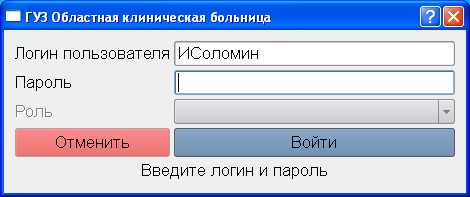
\includegraphics[width = 0.8\textwidth ,keepaspectratio]{p_gen_entry}
 \caption{Окно авторизации пользователя в \tmis}
 \label{img_gen_entry}
\end{figure} 
    
Для начала сеанса работы с \tmis , требуется выполнить вход в систему. Процедура входа в систему называется авторизацией и состоит из следующих шагов:
\begin{enumerate}
\item Запустить приложение \tmis, используя соответствующий ярлык на рабочем столе.
\item В открывшемся окне (Рисунок \ref{img_gen_entry}) нужно ввести идентификатор пользователя, пароль и нажать кнопку \btn{Войти}.
\item Если пользователь в системе выполняет только одну роль, то окно авторизации исчезнет и пользователю станет доступно главное окно программы (Рисунок \ref{img_gen_mw}). В случае если у пользователя имеется несколько ролей, требуется выбрать роль из выпадающего списка (Рисунок \ref{img_gen_entry_rol}) и нажать кнопку  \btn{Выбрать}, после чего пользователю так же станет доступно главное окно программы (Рисунок \ref{img_gen_mw}).
\end{enumerate}
 
\begin{figure}[ht]\centering
 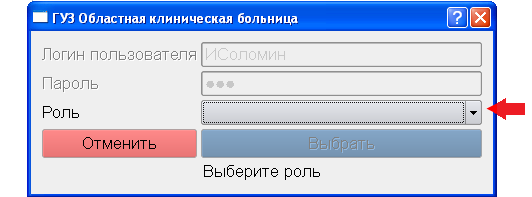
\includegraphics[width = 0.9\textwidth ,keepaspectratio]{p_gen_entry_rol}
 \caption{Выбор роли пользователя}
 \label{img_gen_entry_rol}
\end{figure} 

\begin{figure}[ht]\centering
 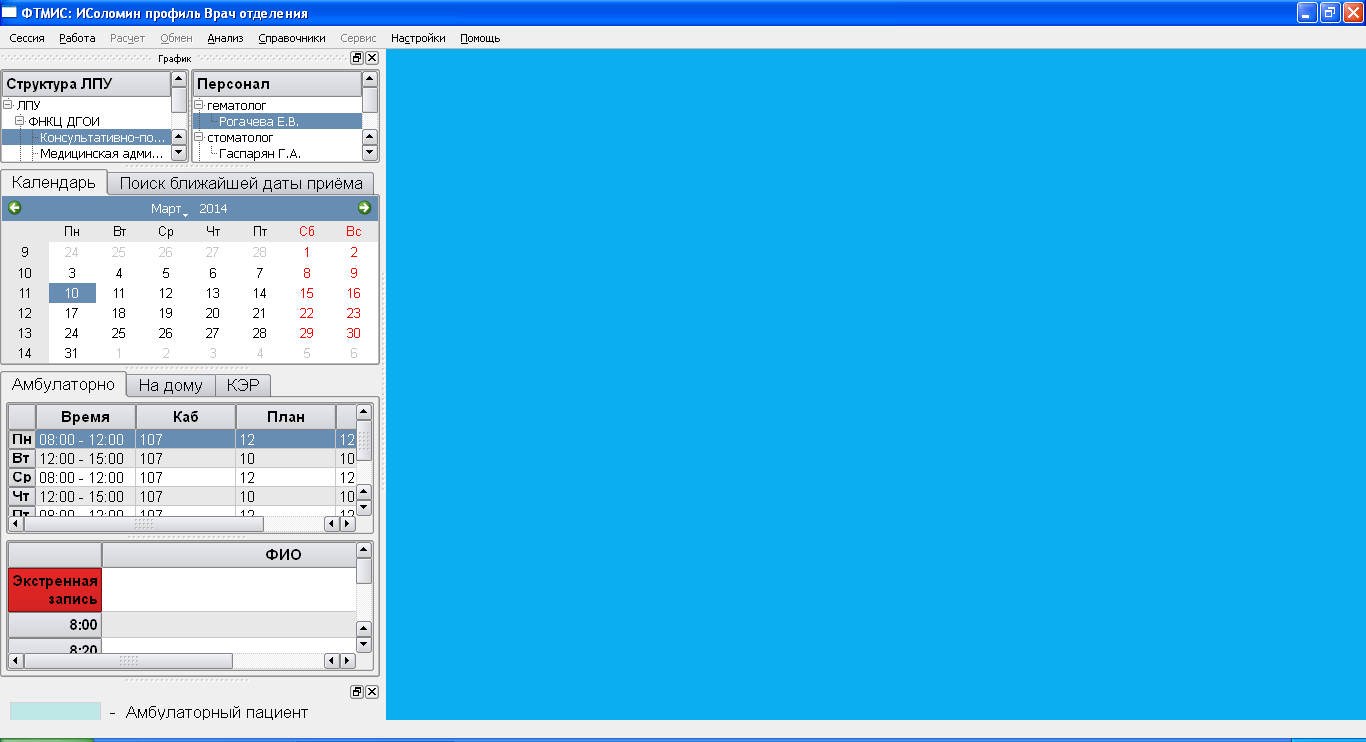
\includegraphics[width = 1\textwidth ,keepaspectratio]{p_gen_mw}
 \caption{Главное окно программы}
 \label{img_gen_mw}
\end{figure} 

Если были введены неверные идентификатор пользователя и (или) пароль, на экране появится сообщение об ошибке (Рисунок \ref{img_gen_entry_err}).

\begin{figure}[ht]\centering
 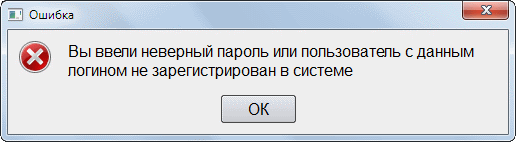
\includegraphics[width = 0.6\textwidth ,keepaspectratio]{p_gen_entry_err}
 \caption{Сообщение об ошибке авторизации}
 \label{img_gen_entry_err}
\end{figure} 

При возникновении данной ошибки рекомендуется:
\begin{itemize}
 \item Проверить язык ввода.
 \item Проверить состояние клавиши \keys{CapsLock} на клавиатуре и выключить ее при необходимости. 
 \item Если в пароле присутствуют цифры, проверить состояние клавиши \keys{NumLock}, включить ее при необходимости.
 \item Повторить попытку авторизации.
\end{itemize}
 
Если проблема не была решена, нужно обратиться к администратору системы для проверки идентификационных данных.

Если в окне авторизации пользователя была нажата кнопка \btn{Отменить} , то основное окно программы останется открытым, но все функции работы в системе будут недоступны. Повторный вход в систему описан в разделе \ref{p_gen_reentry}

\subsubsection{Завершение работы}

\begin{vnim}
Перед закрытием приложения рекомендуется  сохранить все сделанные изменения и закрыть все активные окна.
\end{vnim}

Для выхода из программы необходимо выбрать в главном меню пункт \mm{Сессия \str Закрыть программу} либо нажать кнопку \btn{x}   в правом верхнем углу главного окна. В результате описанных действий программа будет закрыта без дополнительных предупреждений.

\subsubsection{Смена имени пользователя} \label{p_gen_reentry}

Вход в систему под другим именем пользователя можно выполнить не прибегая к закрытию приложения, используя функцию отключения и повторного подключения к базе данных.

Для выхода из системы текущего пользователя нужно в главном меню выбрать \mm{Сессия \str Отключиться от базы данных}. При этом станет недоступной информация на панели слева и большинство пунктов главного меню.

Для входа в систему под новым именем пользователя требуется в главном меню выбрать \mm{Сессия \str Подключиться к базе данных}. На экране появится окно авторизации, куда нужно ввести идентификатор и пароль нового пользователя. Подробно процедура авторизации рассмотрена в разделе \ref{p_gen_entry} Так же рекомендуется использовать команду подключения к базе данных, если во время авторизации пользователя была нажата кнопка \btn{Отменить}.
 %1. Общие сведения
  \newpage
\section{Картотека пациентов}

В \tmis ~для каждого пациента заводится регистрационная карточка, которая содержит всю персональную информацию о пациенте. Она регистрируется в системе при первом обращении пациента в МУ и выполняет функцию амбулаторной карты пациента. При всех последующих обращениях осуществляется поиск ранее зарегистрированной карточки пациента и привязка к ней очередного случая обращения. В случае изменения каких-либо персональных данных пациента, регистрационную карточку можно отредактировать. 

Таким образом, при работе с \tmis~персональные данные пациента вносятся в систему один раз, а медицинские записи добавляются при каждом обращении. Благодаря данному механизму значительно упрощается процесс получение врачом медицинской информации о предыдущих случаях обращения пациента.

Совокупность регистрационных карточек пациентов, случаев их обращений в ЛПУ и результатов обращений называется картотекой пациентов. Для доступа к картотеке пациентов необходимо нажать кнопку \btn{Обслуживание пациентов} на панели управления вверху страницы, либо нажать на блок \dm{Обслуживание пациентов} на главной странице системы (Рисунок \ref{img_gen_main}). Будет осуществлен переход на страницу \dm{Обслуживание пациентов} (Рисунок \ref{img_cl_find}). Здесь можно найти карточку пациента или зарегистрировать нового пациента, просмотреть предварительные записи на прием и данные обращений пациента, а так же зарегистрировать новые.

\begin{figure}[ht]\centering
 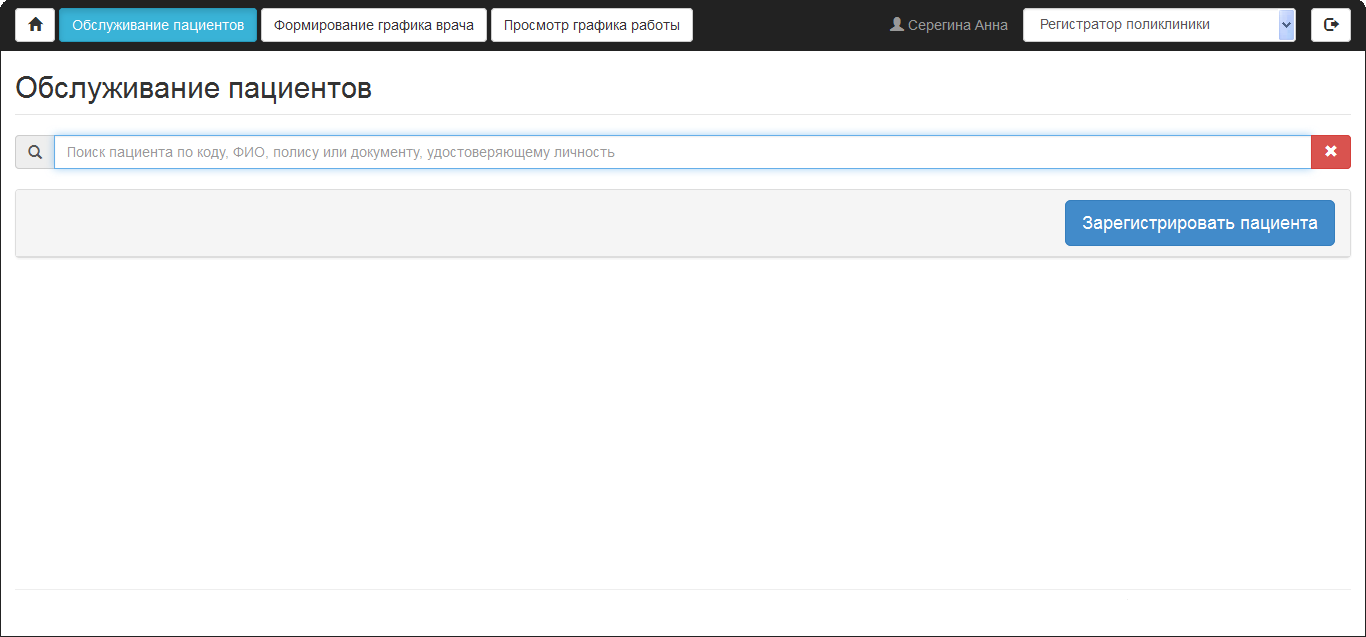
\includegraphics[width = 1\textwidth ,keepaspectratio]{cl_find}
 \caption{Страница поиска и обслуживания пациентов}
 \label{img_cl_find}
\end{figure} 

\subsection{Поиск регистрационной карточки пациента} \label{cl_find}

В верхней части страницы  \dm{Обслуживание пациентов} (Рисунок \ref{img_cl_find}) находится поле для задания параметров поиска пациентов. В него в произвольном порядке можно ввести фамилию, имя, отчество, дату рождения, код пациента, номера его полиса ОМС или документа, удостоверяющего личность. Дату рождения в поле поиска можно вводить в формате <<ДД.ММ.ГГГГ>> либо <<ДДММГГГГ>> без разделителей. 

После ввода всех необходимых критериев поиска, следует нажать клавишу \keys{Enter} на клавиатуре либо кнопку \btn{Найти} в правой части поля поиска. После непродолжительного ожидания на экране появится список найденных согласно заданным условиям пациентов (Рисунок \ref{img_cl_findrez}). 
 
\begin{figure}[ht]\centering
 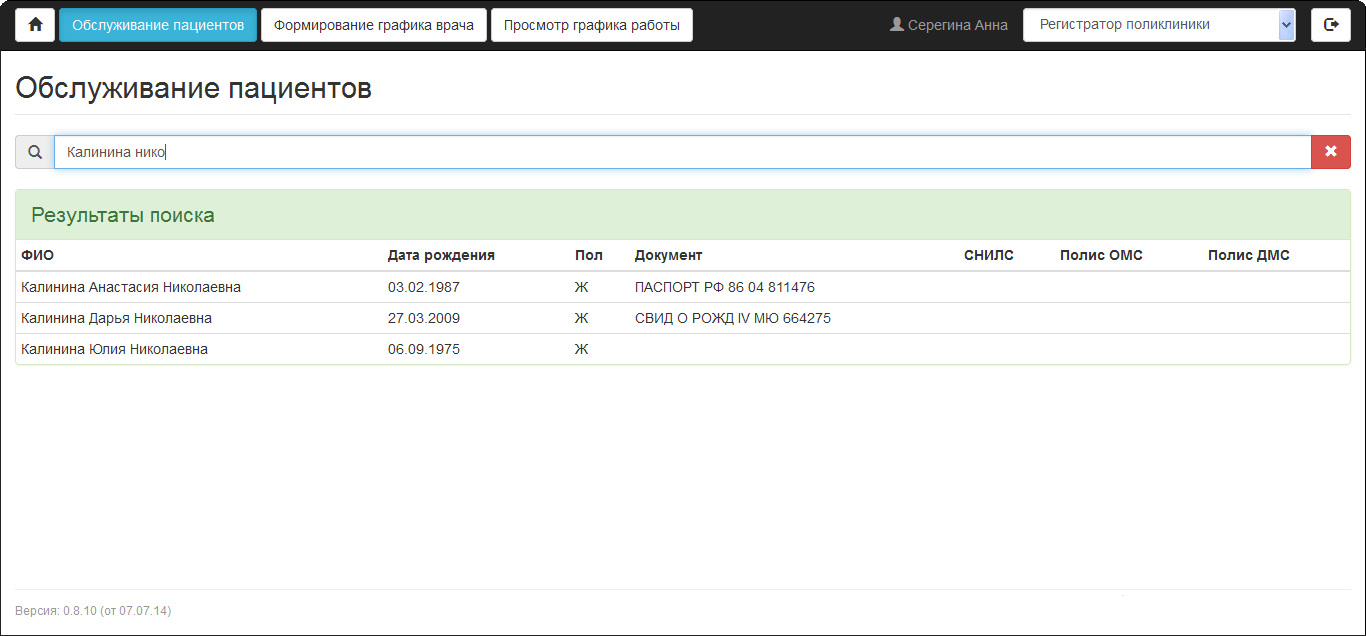
\includegraphics[width = 1\textwidth ,keepaspectratio]{cl_findrez}
 \caption{Результаты поиска пациентов}
 \label{img_cl_findrez}
\end{figure} 

Если по заданным параметрам не будет найдено ни одного пациента, по под полем поиска появится сообщение <<Пациент не найден в базе данных>>.

\ifthenelse{\isnamedefined{fullversion} \OR \isnamedefined{regversion}}
{
\subsection{Регистрационная карточка пациента} \label{cl_card}

Регистрационная карточка пациента содержит всю персональную информацию о пациенте: его фамилию, имя, отчество, дату рождения, адрес, сведения о документах пациента, его страховых полисах, льготах, занятости и т.д. Вся эта информация должна вводиться регистратором с первичных документов пациента при его первом обращении в ЛПУ. В момент регистрации пациента ему присваивается уникальный код, по которому его регистрационную карточку можно быстро найти в картотеке пациентов.

Для регистрации нового пациента необходимо нажать  кнопку \btn{Зарегистрировать пациента} на странице обслуживания пациентов (Рисунок \ref{img_cl_find}). Откроется страница регистрационной карточки пациента (Рисунок \ref{img_cl_card}). 

\begin{figure}[!ht]\centering
 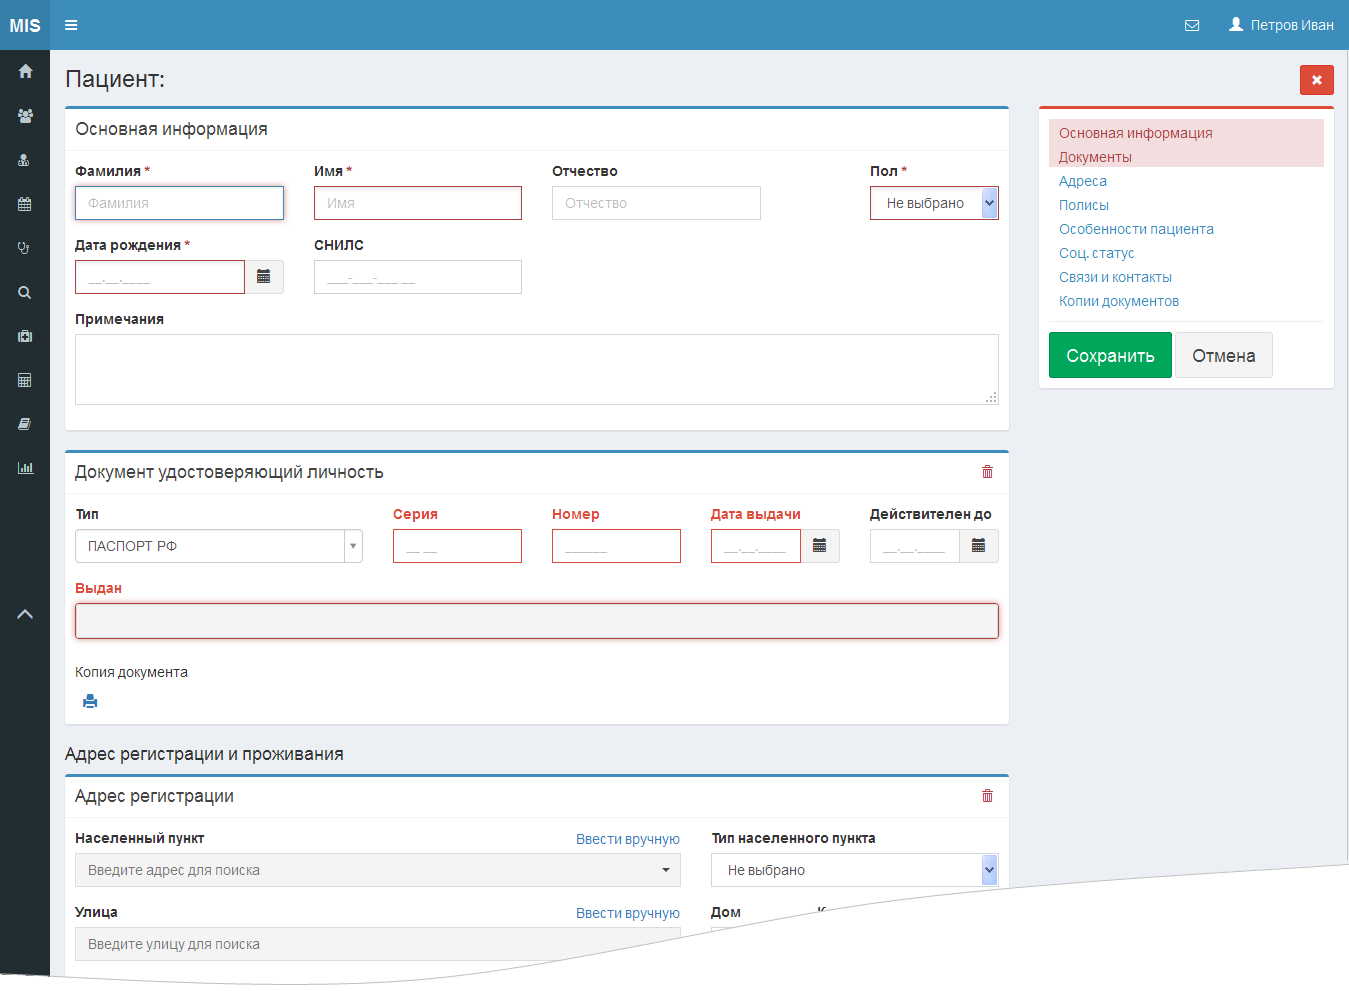
\includegraphics[width = 1\textwidth ,keepaspectratio]{cl_card}
 \caption{Регистрационная карточка пациента}
 \label{img_cl_card}
\end{figure} 

Карточка содержит большое количество информации. Для удобства пользователя, информация разбита на логические блоки. Для перехода к определенному блоку можно щелкнуть левой кнопкой мыши по его названию в левой части страницы либо воспользоваться полосой прокрутки и найти раздел самостоятельно.  

\subsubsection{Блок <<Основная информация>>}

Поля \dm{Фамилия}, \dm{Имя}, \dm{Дата рождения} и \dm{Пол} в регистрационной карточке пациента являются обязательными для заполнения. Они помечены символом <<*>> красного цвета.

Дата рождения пациента может вводиться  с клавиатуры или выбираться из календаря (подрбнее см. раздел \ref{gen_cal}). При заполнении с клавиатуры нужно вводить дату в формате <<ДДММГГГГ>> или <<ДД.ММ.ГГГГ>>. Недостающие разделители вставляются автоматически. Аналогичным образом в \tmis заполняются все поля, содержащие даты.

Значение поля \dm{Пол} может вводиться с клавиатуры или выбираться из раскрывающегося списка. 

В поле \dm{СНИЛС} достаточно ввести только цифры, разделительные тире будут вставлены автоматически. При вводе СНИЛС автоматически проводится проверка корректности введенного значения. В случае, если введенное значение не прошло проверку, поле будет выделено красным цветом и справа от поля появится подсказка <<Введен невалидный СНИЛС>>. Сохранение карточки пациента с неверным СНИЛС невозможно.

В поле \dm{Примечание} можно внести дополнительные сведения о пациенте, для которых не предусмотрено отдельных полей в карточке пациента. 
 
\subsubsection{Блок <<Документ удостоверяющий личность>>}

В данном блоке (Рисунок \ref{img_cl_card}) указываются данные документа, удостоверяющего личность пациента. Как правило, для детей таким документом является свидетельство о рождении, а для взрослых – паспорт. Однако, возможны и другие варианты. 
\begin{itemize}
 \item \dm{Тип документа} выбирается из раскрывающегося списка. В зависимости от выбранного типа, определяется набор реквизитов документа, доступных и обязательных для  заполнения. Обязательные для заполнения поля подсвечиваются красным цветом. Для большинства типов документов обязательно требуется указать серию, номер, дату выдачи и кем был выдан документ. 
 \item \dm{Серия, Номер}. Для каждого типа документов задается собственный формат серии и номера: определяется их длина,  возможность ввода в поле буквенных значений, а так же других специальных символов. 
 \item В поле \dm{Дата выдачи} дата может вводиться с клавиатуры или выбираться из календаря (подробнее см. раздел \ref{gen_cal}) 
 \item Поле \dm{Действителен до} заполняется аналогично предыдущему. Если документ не имеет срока действия, то поле может оставаться пустым. Данное поле необходимо заполнить обязательно, если в \tmis~происходит изменение сведений о действующем документе, удостоверяющем личность (т.е. если пациент предоставил новый документ того же типа, что и предыдущий). 
 \item В поле \dm{Выдан} можно выбрать значение из справочника или ввести произвольный текст с клавиатуры. По мере ввода текста в данное поле, в его  раскрывающемся списке будет производиться фильтрация значений в соответствии с введенным текстом. Для выбора значения из справочника необходимо щелкнуть по нему левой кнопкой мыши или переместить на него курсор с помощью стрелок на клавиатуре, а затем нажать клавишу \keys{Enter}. Для сохранения значения не из справочника необходимо обязательно нажать клавишу \keys{Enter} в данном поле после завершения ввода. Для очистки поля нужно нажать кнопку 
\includegraphics[scale=0.6]{clear} в правой части поля.
\end{itemize}

После сохранения информации о документе, удостоверяющем личность пациента появляется возможность прикрепления скан-копии указанного документа (Рисунок \ref{img_cl_docs}). Для этого необходимо нажать кнопку \btn{Добавить копию документа} в нижней части данного блока и в появившемся всплывающем окне выполнить прикрепление документа со сканера или из файла (см. раздел \ref{cl_copydocs}).  

\begin{figure}[ht]\centering
 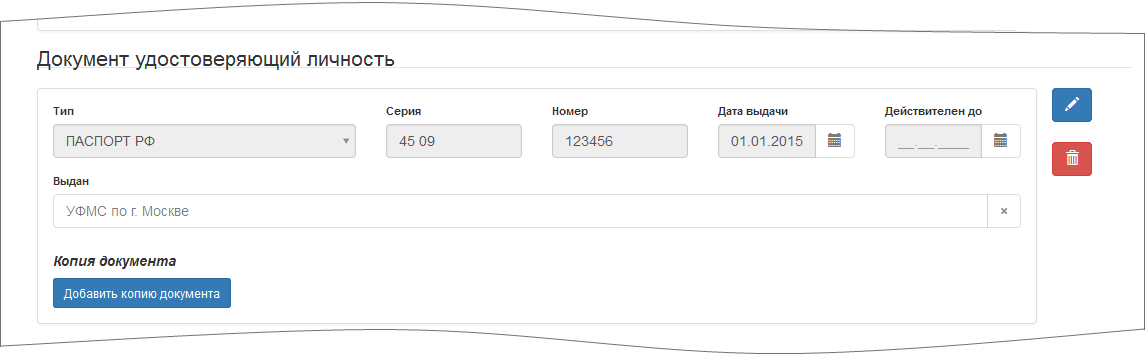
\includegraphics[width = 1\textwidth ,keepaspectratio]{cl_docs}
 \caption{Регистрационная карточка пациента. Блок ввода документа, удостоверяющего личность}
 \label{img_cl_docs}
\end{figure} 

\subsubsection{Блок <<Адрес регистрации и проживания>>}

В регистрационной карточке существует возможность указания двух адресов для каждого пациента: адреса регистрации и адреса фактического проживания (Рисунок \ref{img_cl_adres}). 

\begin{figure}[ht]\centering
 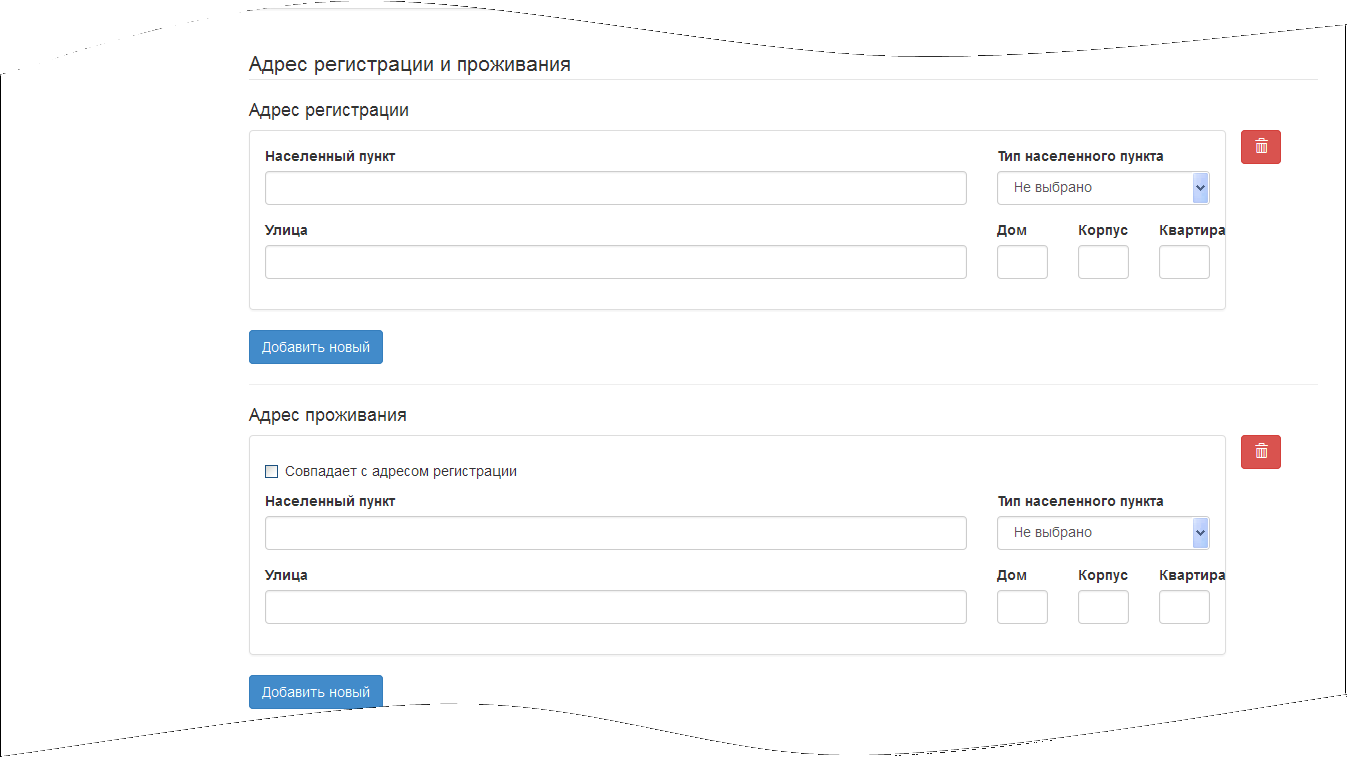
\includegraphics[width = 1\textwidth ,keepaspectratio]{cl_adres}
 \caption{Регистрационная карточка пациента. Блок ввода адреса регистрации.}
 \label{img_cl_adres}
\end{figure} 

Заполнение адреса рекомендуется выполнять с помощью всероссийского классификатора адресов -- КЛАДР. Для заполнения полей \dm{Населенный пункт} или \dm{Улица} нужно ввести его(ее) наименование или часть наименования в соответствующее поле и нажать клавишу \keys{Enter} на клавиатуре. В раскрывающемся списке поля появится перечень наименований, найденных в соответствии с условиями поиска. Необходимо выбрать из раскрывающегося списка требуемое значение, щелкнув по нему левой кнопкой мыши или установив на него курсор с помощью стрелок на клавиатуре и нажав клавишу \keys{Enter}. Поля \dm{Дом}, \dm{Корпус} и \dm{Квартира} могут заполняться произвольными значеними.

Если для данных, внесенных в поля \dm{Населенный пункт} и \dm{Улица}, не найдены соответствия в справочнике КЛАДР, то поля будут считаться заполненными с ошибками. Они будут подсвечены красным цветом, а в верхней части блока появится сообщение об ошибке <<Введенный адрес не найден в справочнике адресов Кладр. Ввести адрес вручную?>> (Рисунок \ref{img_cl_adrf}). Сохранение карточки пациента при этом будет невозможно. 

\begin{figure}[ht]\centering
 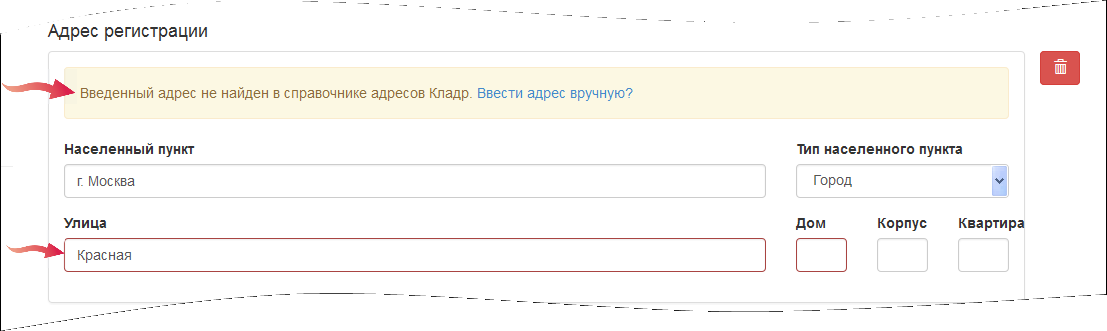
\includegraphics[width = 1\textwidth ,keepaspectratio]{cl_adrf}
 \caption{Регистрационная карточка пациента. Блок ввода адреса регистрации. Адрес не найден в справочнике КЛАДР}
 \label{img_cl_adrf}
\end{figure} 

В такой ситуации следует еще раз проверить правильность написания названий населенного пункта и улицы, попытаться использовать другое написание или альтернативные названия. Если и после этого найти соответствие в справочнике не удалось, можно щелкнуть левой кнопкой мыши по фразе <<Ввести адрес вручную?>> в тексте сообщения об ошибке. Поля  \dm{Населенный пункт}, \dm{Улица}, \dm{Дом}, \dm{Корпус} и \dm{Квартира} при этом станут недоступными для редактирования, но появится новое поле \dm{В свободном виде} в нижней части блока, куда можно будет ввести адрес в произвольной форме. Проверка на соответствие справочнику КЛАДР при этом производиться не будет (Рисунок \ref{img_cl_adrfree}). 

\begin{vnim}
Ввод адреса в свободной форме можно применять только в крайних случаях, если выбор из справочника КЛАДР абсолютно невозможен. 
\end{vnim}

\begin{figure}[ht]\centering
 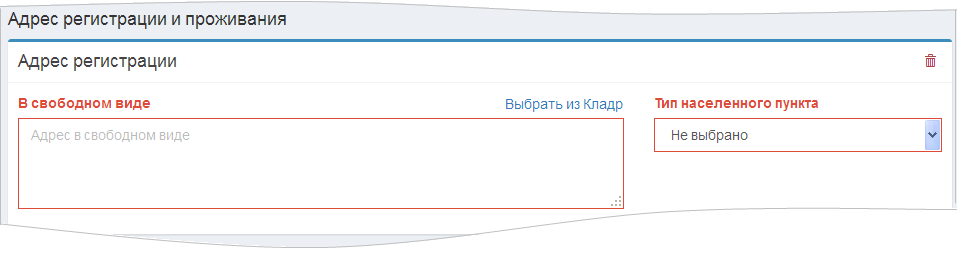
\includegraphics[width = 1\textwidth ,keepaspectratio]{cl_adrfree}
 \caption{Регистрационная карточка пациента. Блок ввода адреса регистрации. Ввод адреса в свободной форме}
 \label{img_cl_adrfree}
\end{figure}   

\begin{prim}
Для того, чтобы от свободного ввода снова вернуться к вводу адреса по справочнику КЛАДР, нужно щелкнуть в сообщении об ошибке вверху блока по фразе <<Выбрать из Кладр>>. При этом поле \dm{В свободном виде} исчезнет, а остальные поля снова станут доступны для редактирования.
\end{prim}

В полях ниже, аналогичным способом можно ввести адрес фактического проживания пациента. Если адрес фактического проживания совпадает с адресом регистрации, то в подразделе \dm{Адрес проживания} можно установить флажок \dm{Совпадает с адресом регистрации}. Тогда данные из подраздела \dm{Адрес регистрации} будут скопированы в соответствующие поля подраздела \dm{Адрес проживания}. Редактирование адреса проживания при этом становится недоступно. 
 
\subsubsection{Блок <<Медицинские полисы>>}
  
В подразделе \dm{Полис ОМС} (Рисунок \ref{img_cl_police}) указываются данные действующего полиса обязательного медицинского страхования. Необходимо указать тип полиса, его серию и номер, дату выдачи, срок действия и название СМО, выдавшей полис. Поле \dm{Действителен до} может оставаться незаполненным, если срок действия полиса не ограничен. Остальные поля являются обязательными для заполнения. 

В поле \dm{Страховая медицинская организация} можно выбрать наименование из справочника или ввести произвольное значение с клавиатуры. По мере ввода текста в данное поле, в его  раскрывающемся списке будет производиться фильтрация значений в соответствии с введенным текстом. Для выбора значения из справочника необходимо щелкнуть по нему левой кнопкой мыши или установить на него курсор с помощью стрелок на клавиатуре, а затем нажать клавишу \keys{Enter}. Для сохранения значения отсутствуюшего в справочнике требуется нажать клавишу \keys{Enter} в данном поле после завершения ввода. Для очистки поля нужно нажать кнопку 
\includegraphics[scale=0.6]{clear} в правой части поля.

\begin{figure}[ht]\centering
 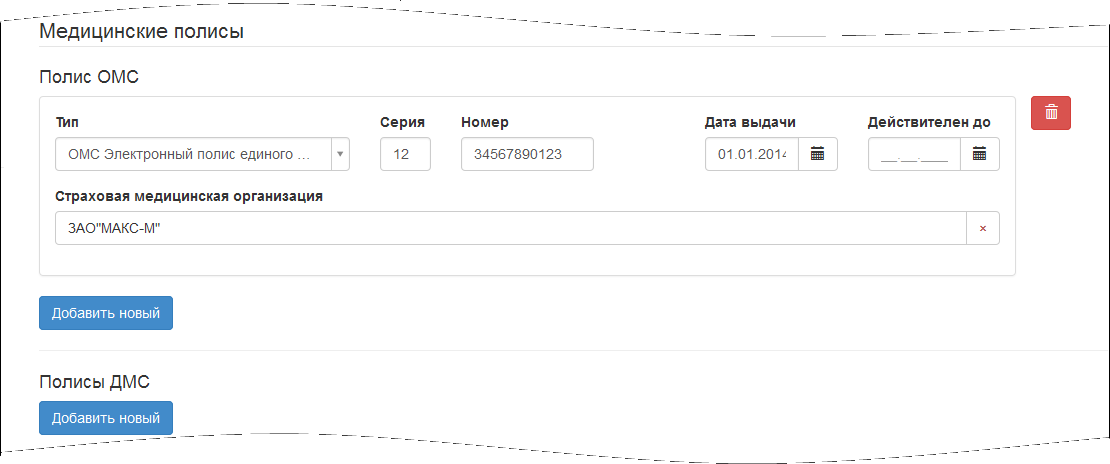
\includegraphics[width = 1\textwidth ,keepaspectratio]{cl_police}
 \caption{Регистрационная карточка пациента. Блок ввода полисов пациента.}
 \label{img_cl_police}
\end{figure}  

В подразделе \dm{Полис ДМС} по умолчанию поля скрыты. Для добавления полиса ДМС в карточку пациента необходимо нажать кнопку \btn{Добавить новый} в подразделе \dm{Полисы ДМС}. Появятся поля, аналогичные полям в подразделе \dm{Полис ОМС}. Заполнение данных полиса ДМС осуществляется аналогично заполнению раздела \dm{Полисы ОМС}.

Пациент может иметь только один действующий полис ОМС и любое количество действующих полисов ДМС. Поэтому при добавлении нового полиса ОМС, он заменяет ранее зарегистрированный. При добавлении нового полиса ДМС он добавляется к списку существующих полисов ДМС. 

\begin{prim}
При изменении данных полиса или документа, удостоверяющего личность, ранее введенные данные не теряются. Все ранее зарегистрированные для пациента полисы  и документы, удостоверяющие личность, можно найти в блоке \dm{История изменений документов} (см.раздел \ref{cl_docshistory})
\end{prim}

После сохранения данных полиса, можно прикрепить фотокопию данного документа к регистрационной карточке. Для этого необходимо нажать кнопку \btn{Добавить копию документа} в конце соответствуюшего подраздела и выполнить прикрепление документа со сканера либо из файла (см. раздел \ref{cl_copydocs})


\subsubsection{Блок <<Особенности пациента>>} 

Блок \dm{Особенности пациента} содержит жизненно-важные параметры, необходимые для оказания медицинской помощи (витальную информацию): группу крови, сведения об аллергии и медикаментозной непереносимости (Рисунок \ref{img_cl_osob}). 

\begin{figure}[!ht]\centering
 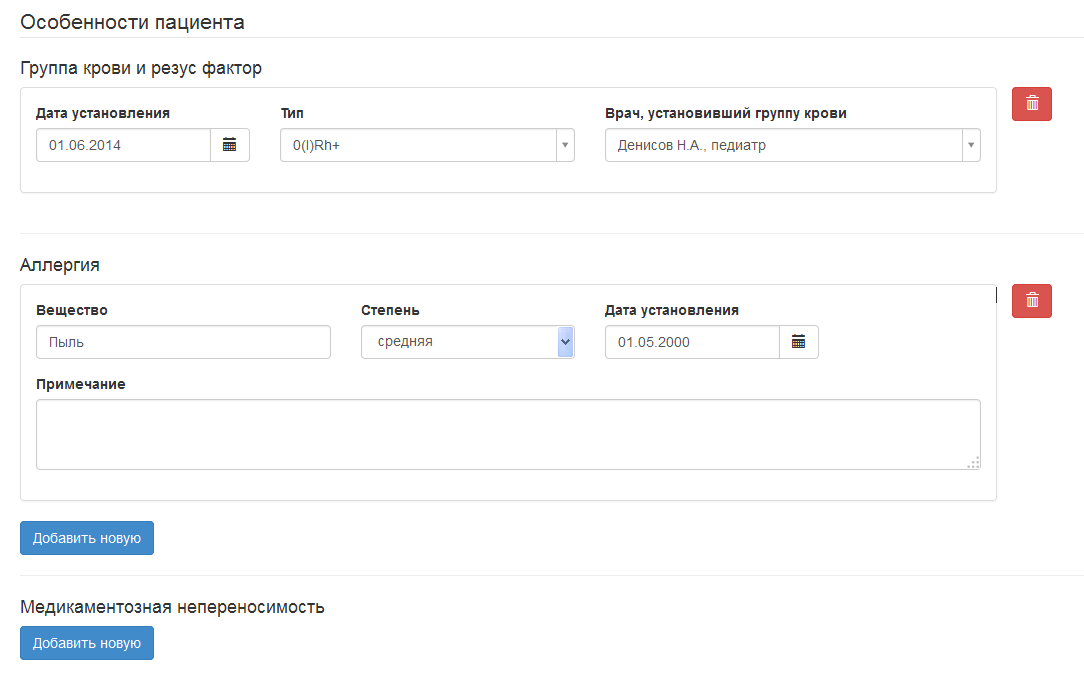
\includegraphics[width = 1\textwidth ,keepaspectratio]{cl_osob}
 \caption{Регистрационная карточка пациента. Блок <<Особенности пациента>>}
 \label{img_cl_osob}
\end{figure} 

Блок содержит 3 подраздела: 
\begin{itemize}
 \item Группа крови и резус фактор;
 \item Аллергия;
 \item Медикаментозная непереносимость.
\end{itemize}

По умолчанию поля для каждого из подразделов скрыты. Для добавления информации в какой-либо из подразделов нходимоеобходимо нажать кнопку \btn{Добавить новую}. Тогда на странице появятся дополнительные поля для ввода информации соответствующего подраздела.

В подразделе \dm{Группа крови и резус-фактор} хранится информация о группе крови  и резусе пациента. Если группа крови пациента известна, то ее необходимо внести в регистрационную карточку. Для этого следует нажать кнопку \btn{Добавить новую} и заполнить появившиеся поля. В поле \dm{Дата установления} нужно указать дату установления группы крови, в поле \dm{Тип} следует выбрать группу крови и резус-фактор из справочника, в поле \dm{Врач, установивший группу крови} выбрать фамилию врача из справочника сотрудников (по умолчанию указывается фамилия текущего пользователя). Все поля обязательны для заполнения. 

Если группа крови была установлена в другом МУ, то в качестве врача, установившего группу крови, следует указывать сотрудника, зарегистрировавшего ее в карточке пациента.

\begin{vnim}
Редактирование группы крови и резус-фактора после сохранения регистрационной карточки пациента становится невозможным. Проявите особую аккуратность при внесении этих данных.
\end{vnim}

Подразделы \dm{Аллергия} и \dm{Медикаментозная непереносимость} заполняются по одному и тому же принципу. В поле  \dm{Вещество (Препарат)} необходимо ввести описание аллергена, например <<пыль>> или <<ампициллин>>, в ячейке \dm{Степень} выбрать из списка степень аллергической реакции, в ячейке \dm{Дата установления} ввести дату установления аллергии (медикаментозной непереносимости), в поле \dm{Примечание}, можно указать дополнительные сведения относительно реакции. В каждом подразделе может содержаться любое количество записей. Добавление новых записей производится нажатием кнопки \btn{Добавить новую}. Поля \dm{Вещество (Препарат)}, \dm{Степень} и \dm{Дата установления} являются обязательными для заполнения. В случае их незаполнения, поля будут подсвечиваться красным цветом, сохранение регистрационной карточки пациента при этом будет невозможно.

\subsubsection{Блок <<Социальные статусы>>} 

В этом блоке можно внести ряд дополнительных сведений о пациенте, которые используются, в первую очередь для статистического учета (Рисунок \ref{img_cl_socst}): 
\begin{itemize}
 \item \dm{Инвалидность} -- данные о виде инвалидности пациента и документах, подтверждающих ее.
 \item \dm{Занятость} -- сведения о занятости пациента.
 \item \dm{Гражданство}.
\end{itemize}

По умолчанию поля для каждого из подразделов скрыты. Для добавления информации в какой-либо из подразделов необходимо нажать кнопку \btn{Добавить инвалидность}, \btn{Добавить занятость} или \btn{Добавить гражданство} соответственно.

\begin{figure}[ht]\centering
 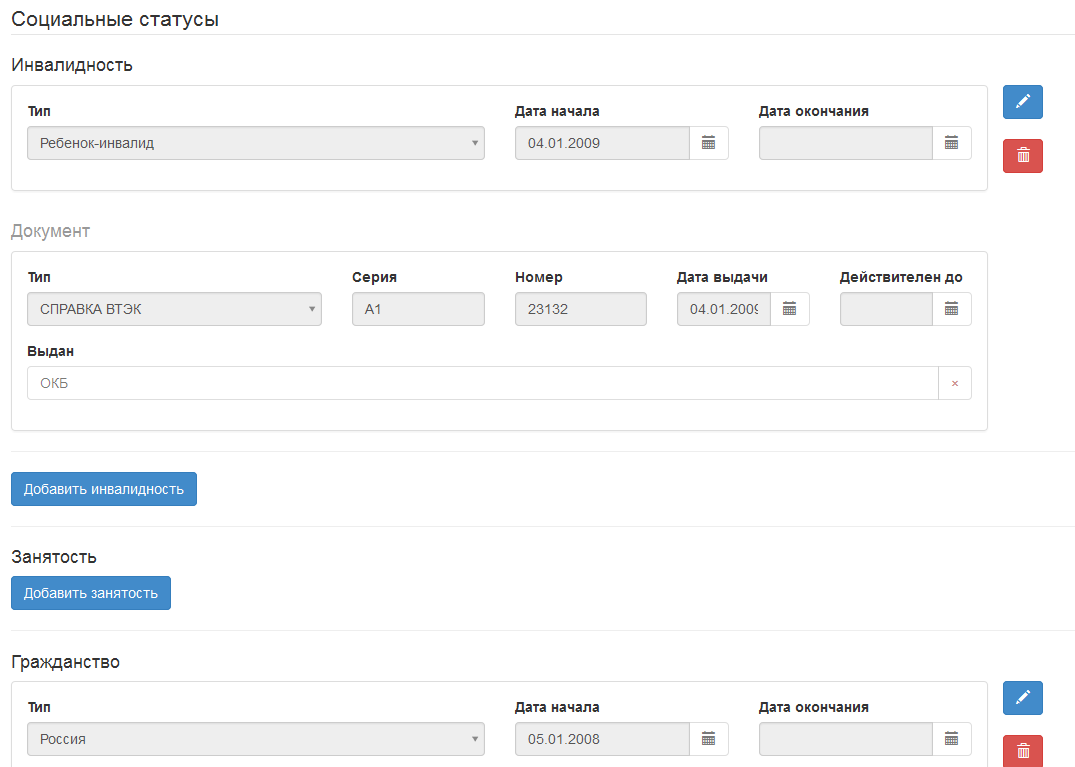
\includegraphics[width = 1\textwidth ,keepaspectratio]{cl_socst}
 \caption{Регистрационная карточка пациента. Блок <<Социальные статусы>>}
 \label{img_cl_socst}
\end{figure} 

При заполнении данных перечисленных подразделов необходимо выбрать значение в поле \dm{Тип} и указать дату в поле \dm{Дата начала}. Если настоящая дата установления статуса (например, гражданства) неизвестна, то можно указать текущую дату. Для инвалидности обязательно следует указывать настоящую дату установления в поле \dm{Дата начала}, а так же ввести данные документа, подтверждающего инвалидность.


\begin{prim}
Данные обо всех документах, подтверждающих инвалидность можно так же просмотреть в блоке \dm{История изменений документов} (см. раздел \ref{cl_docshistory}).
\end{prim}
 
\subsubsection{Блок <<Контактная информация и родственники>>}

В подраздел \dm{Связи с другими пациентами} содержит указатели на регистрационные карточки родственников пациента (Рисунок \ref{img_cl_contact}). 

\begin{vnim}
Для создания связи родственник должен быть зарегистрирован в \tmis.
\end{vnim}

\begin{figure}[ht!]\centering
 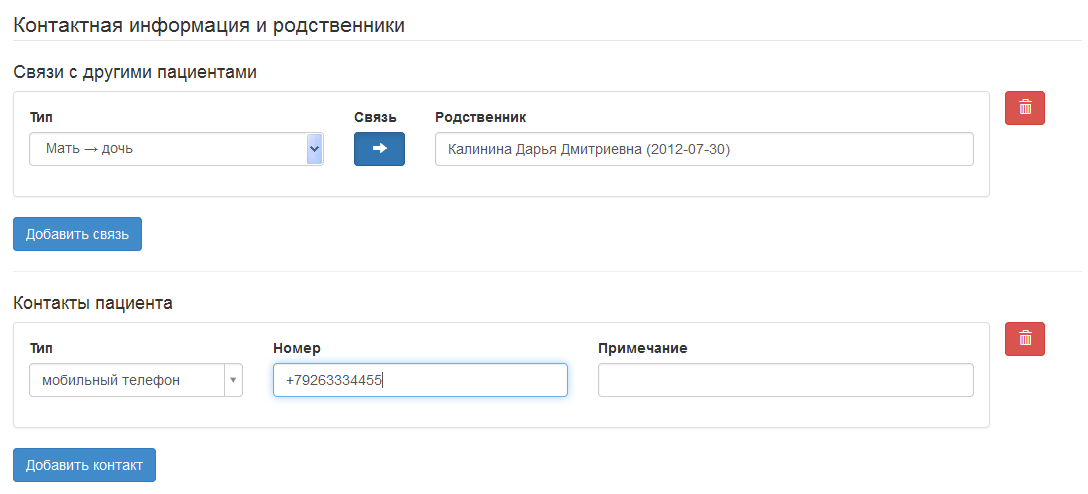
\includegraphics[width = 1\textwidth ,keepaspectratio]{cl_contact}
 \caption{Регистрационная карточка пациента. Блок <<Контактная информация и родственники>>}
 \label{img_cl_contact}
\end{figure} 

Для добавления связи необходимо нажать кнопку \btn{Добавить связь}, выбрать тип связи в поле \dm{Тип} и соответствующего пациента из БД в поле \dm{Родственник}. Список доступных значений в поле \dm{Тип} определяется значением в поле \dm{Пол} для текущего пациента, а так же направлением стрелки в поле \dm{Связь}. Для изменения направления связи необходимо щелкнуть по кнопке с изображением стрелки в поле \dm{Связь}. Для поиска родственника необходимо ввести его фамилию в поле \dm{Родственник}. По мере набора фамилии будет осуществляться поиск пациентов в БД. Результат поиска будет отображаться в раскрывающемся списке поля. Следует выбрать из этого списка нужного пациента. Если не будет найдено соответствия введенных данных с пациентами в БД, поле \dm{Родственник} будет подсвечено красным цветом. Сохранение регистрационной карточки пациента при этом будет невозможно.

Возможен ввод нескольких родственников в карточку пациента. Для добавления нового родственника следует нажать кнопку \btn{Добавить связь} и внести данные во вновь открывшиеся поля.

В подразделе \dm{Контакты пациента} можно хранить контактные данные пациента: номера телефонов, факсов, данные контактных лиц, адреса электронной почты и т.п.

Для добавления контактной информации следует нажать кнопку \dm{Добавить контакт}, затем во вновь открывшиеся поля ввести следующие данные: в поле \dm{Тип} выбрать тип контактной информации, в поле \dm{Номер} ввести номер телефона, факса, адрес электронной почты, в поле \dm{Примечание} можно указать любую дополнительную информацию относительно контакта, например, имена родственников, рекомендуемое время звонка и т.д.

Возможен ввод нескольких контактов в карточку пациента. Для добавления нового контакта следует нажать кнопку \btn{Добавить контакт} и внести данные во вновь открывшиеся поля.


\subsubsection{Копии документов} \label{cl_copydocs}

В данном блоке можно добавить или просмотреть фотокопии документов пациента, прикрепленные к карточке (Рисунок \ref{img_cl_copydocs}). 

\begin{figure}[ht!]\centering
 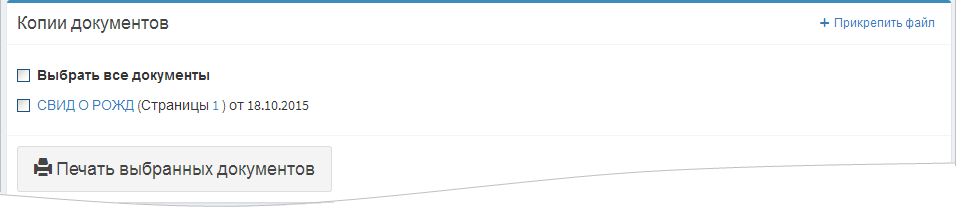
\includegraphics[width = 1\textwidth ,keepaspectratio]{cl_copydocs}
 \caption{Регистрационная карточка пациента. Блок <<Копии документов>>}
 \label{img_cl_copydocs}
\end{figure} 

Добавление копий документов может производиться как в данном блоке, так и в блоке, соответствующем типу сохраняемого документа. Для добавления документа из данного блока нужно нажать кнопку \btn{Прикрепить файл}. Для добавления копии документа из блока, соответствующего типу добавляемого документа,  необходимо нажать кнопку \btn{Добавить копию документа} в конце соответствующего типу документа раздела или блока. Данная кнопка доступна только после сохранения информации о документе пациента. После нажатия на кнопку появляется  всплывающее окно(Рисунок \ref{img_cl_addcopydoc}), где имеется возможность прикрепления копии документа непосредственно со сканера или из ранее сохраненного файла.

\begin{figure}[ht]\centering
 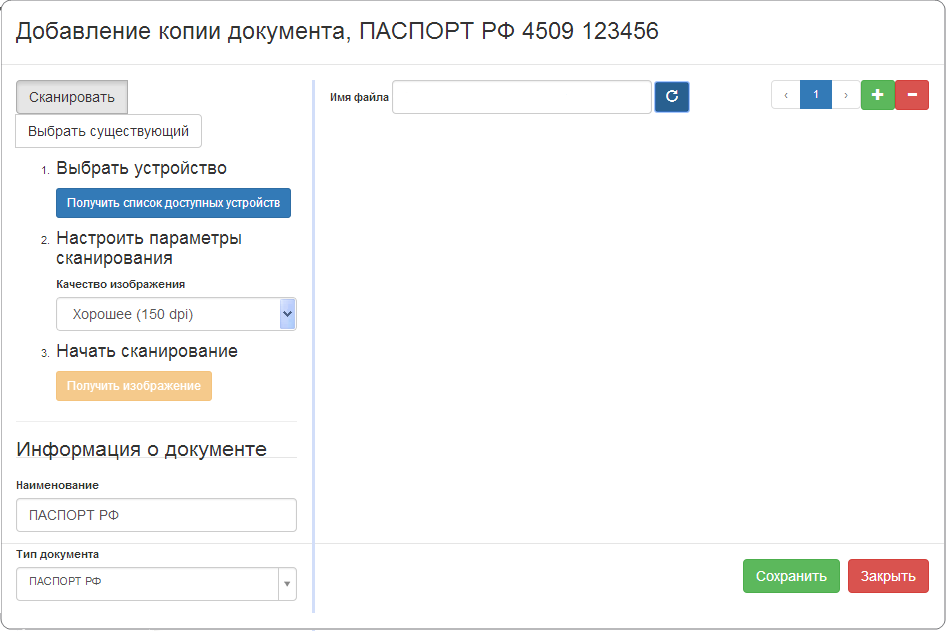
\includegraphics[width = 1\textwidth ,keepaspectratio]{cl_addcopydoc}
 \caption{Добавление копии документа со сканера}
 \label{img_cl_addcopydoc}
\end{figure} 

Для получения копии документа со сканера необходимо нажать <<Сканировать>> в левом верхнем углу окна (выбирается по умолчанию) (Рисунок \ref{img_cl_addcopydoc}). При отсутствии сканера в списке устройств в окне требуется нажать кнопку \btn{Получить список доступных устройств}. После непродолжительной обработки под кнопкой появится список устройств, подключения к которым обнаруженны на данном компьютере. Необходимо установить переключатель на устройство-сканер, выбрать качество сканирования в раскрывающемся списке ниже и нажать кнопку \btn{Получить избражение}. Начнется процесс сканирования, который может занять несколько секунд. После его завершения скан-копия документа появится в правой части всплывающего окна.

Для сохранения копии документа из файла необходимо нажать <<Выбрать существующий>> в левом верхнем углу окна. Далее следует нажать кнопку \btn{Выберите файл} и в появившемся окне указать путь к ранее сохраненной фотокопии документа. После загрузки файла в систему, он так же отобразится в правой части окна (Рисунок \ref{img_cl_addcopydoc2}).   

\begin{figure}[ht]\centering
 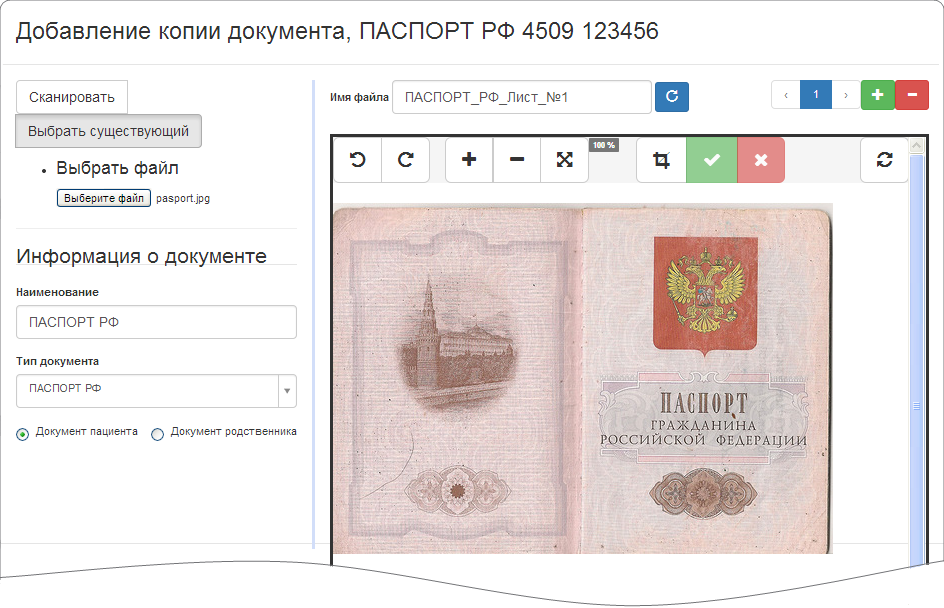
\includegraphics[width = 1\textwidth ,keepaspectratio]{cl_addcopydoc2}
 \caption{Добавление копии документа из файла}
 \label{img_cl_addcopydoc2}
\end{figure} 

Далее следуют заполнить подраздел \dm{Информация о документе} в левой части всплывающего окна:
\begin{itemize}
 \item \dm{Тип документа} -- выбирается из справочника типов документов и должен соответствовать типу прикрепляемого документа.
 \item \dm{Наименование} -- наименование документа, которое будет отображаться в регистрационной карточке пациента. По умолчанию наименование совпадает с выбранным типом документа, но можно ввести произвольное наименование.
 \item Принадлежность прикрепляемого документа выбирается переключателем: документ пациента либо его родственника.
\end{itemize}

В правой части окна находятся следующие управляющие элементы:
\begin{itemize}
 \item \dm{Имя файла} -- имя текущего листа документа. С помощью кнопки 
\includegraphics[scale=0.7]{cpdrefresh} в конце поля можно сформировать автоматическое имя листа.
 \item Кнопки 
\includegraphics[scale=0.7]{cpdadd} и 
\includegraphics[scale=0.7]{cpddel} позволяют добавить и удалить соответственно страницы документа. На каждой странице возможно размещение только одного изображения. При попытке добавить новое изображение на ту же страницу, предыдущее будет удаляться. Таким образом, для сохранения копий нескольких страниц документа, необходимо добавлять соответствующее число страниц. Удаление страницы приводит к удалению размещенного на ней изображения.
 \item Кнопки навигации  
\includegraphics[scale=0.9]{cpdnavi} позволяют перемещаться по страницам документа. Для перемещения можно щелкнуть по номеру страницы либо воспользоваться стралками влево и право для последовательного перехода по страницам. 
\end{itemize}

После внесения всей необходимой информации нужно сохранить ее, нажав кнопку \btn{Сохранить} в правом нижнем углу всплывающего окна. В поле \dm{Копия документа} соответствующего блока регистрационной карточки пациента, а так же в текущем разделе, появится ссылка на прикрепленное изображение (Рисунок \ref{img_cl_addcopydoc3}). Для просмотра и редактирования прикрепленной фотокопии следует щелкнуть по наименованию документа левой кнопкой мыши. 

\begin{figure}[ht]\centering
 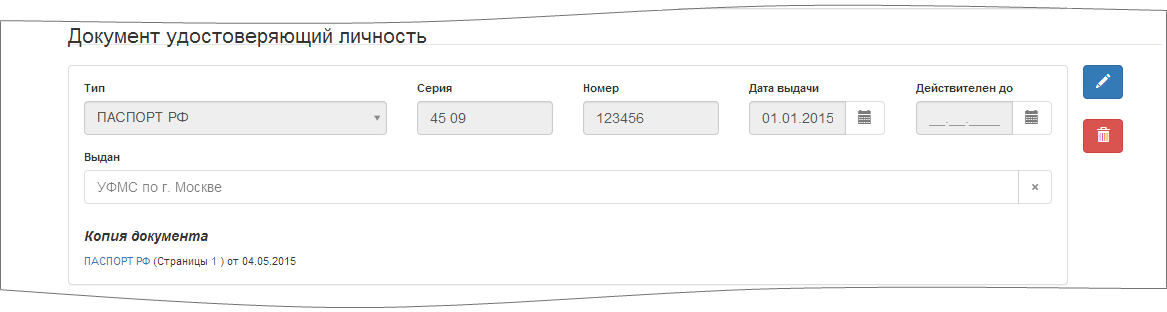
\includegraphics[width = 1\textwidth ,keepaspectratio]{cl_addcopydoc3}
 \caption{Информация о прикреплении копии документа в регистрационной карточке пациента}
 \label{img_cl_addcopydoc3}
\end{figure} 
  

\subsubsection{Блок <<История изменения документов>>} \label{cl_docshistory}

В данном блоке содержится информация обо всех документах, которые когда-либо регистрировались для данного пациента (Рисунок \ref{img_cl_docshistory}). В истории учитываются документы, удостоверяющие личность пациента, полиса ОМС и ДМС, документы, подтверждающие социальные статусы пациента. Для каждого документа указывается его тип, серия, номер, дата начала и окончания действия. Список документов доступен только для просмотра. Редактирование и удаление документов невозможно. 

\begin{figure}[ht]\centering
 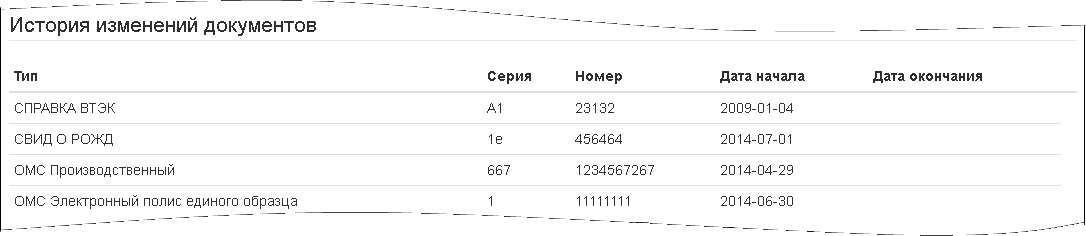
\includegraphics[width = 1\textwidth ,keepaspectratio]{cl_docshistory}
 \caption{Регистрационная карточка пациента. Блок <<История изменений документов>>}
 \label{img_cl_docshistory}
\end{figure} 


\subsection{Регистрация нового пациента} \label{cl_new}

Для регистрации нового пациента необходимо в верхней части страницы нажать кнопку \btn{Обслуживание пациентов}, после чего нажать кнопку \btn{Зарегистрировать пациента}  в правой верхней части открывшейся страницы.

\begin{vnim}
Перед началом регистрации нового пациента необходимо убедиться, что данный пациент не был зарегистрирован ранее. Для этого рекомендуется воспользоваться поиском (см. раздел \ref{cl_find})
\end{vnim}

После нажатия кнопки \btn{Зарегистрировать пациента} откроется страница регистрационной карточки пациента,  содержащая незаполненные поля. Необходимо ввести все данные пациента в пустые поля в соответствии с разделом \ref{cl_card} Для сохранения введенных данных требуется нажать кнопку \btn{Сохранить} в левой части страницы.

Если какие-либо поля регистрационной карточки были заполнены неправильно или некоторые обязательные для заполнения поля остались пустыми, сохранение будет невозможно. В этом случае, при нажатии на кнопку \btn{Сохранить}, рядом с ней появится соответствующая подсказка.

Если сохранение карточки не требуется, нужно нажать кнопку \btn{Отмена} в левой части страницы. Страница регистрации пациента будет закрыта без сохранения данных в БД.

Перемещение между блоками регистрационной карточки можно выполнять как с помощью полос прокрутки или колесика мыши, так и с помощью ссылок на блоки, расположенных в левой части страницы регистрационной карточки пациента (Рисунок \ref{img_cl_content}). Для того, чтобы перейти к нужному блоку с помощью ссылки, достаточно щелкнуть по ней левой кнопкой мыши.

\begin{figure}[ht]\centering
 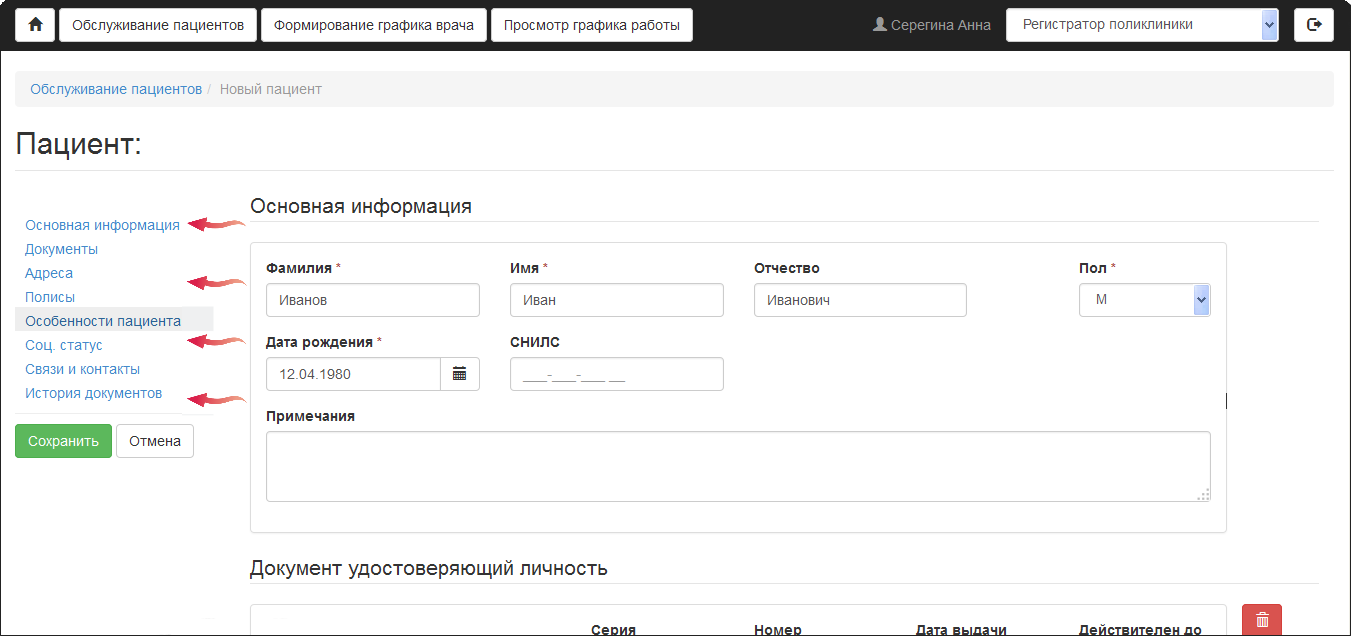
\includegraphics[width = 1\textwidth ,keepaspectratio]{cl_content}
 \caption{Ссылки на блоки регистрационной карточки}
 \label{img_cl_content}
\end{figure} 

\subsection{Редактирование регистрационной карточки пациента}

Данные, введенные в регистрационную карточку пациента, не являются статичными, их можно динамически изменять в соответствии с изменениями и уточнениями персональных данных пациента. При изменении каких-либо документов у пациента, его социального статуса, выявлении новых особенностей и т.п., требуется открыть регистрационную карточку пациента на редактирование и внести в нее соответствующие изменения. 

Для редактирования регистрационной карточки пациента, следует найти пациента в БД (см. раздел \ref{cl_find}), щелкнуть по записи о нем левой кнопкой мыши (Рисунок \ref{img_cl_findrez}) и в появившемся всплывающем окне (Рисунок \ref{img_cl_contrwin}) нажать кнопку \btn{Редактировать данные пациента} или кнопку 
\includegraphics[scale=0.6]{edt} в правом верхнем углу окна. 
}{}

\begin{figure}[ht]\centering
 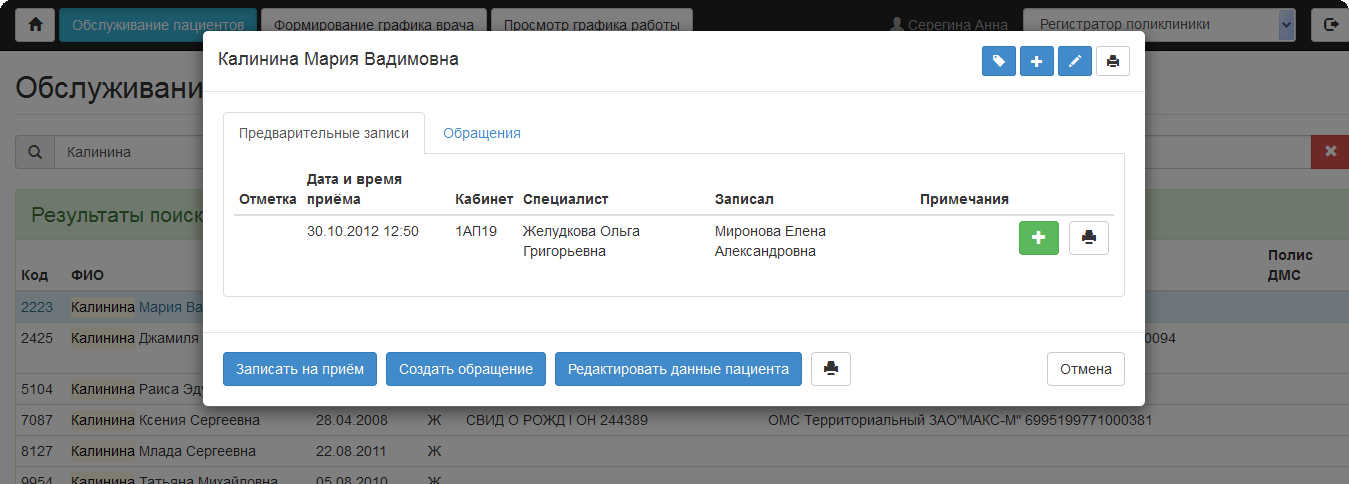
\includegraphics[width = 1\textwidth ,keepaspectratio]{cl_contrwin}
 \caption{Окно управления обслуживанием пациента}
 \label{img_cl_contrwin}
\end{figure} 

\ifthenelse{\isnamedefined{fullversion} \OR \isnamedefined{regversion}}{
Откроется страница, содержащая заполненную регистрационную карточку пациента. Требуется внести изменения в соответствующие поля и сохранить их, нажав кнопку \btn{Сохранить}. Состав полей и методы их заполнения подробно рассмотрены в разделе \ref{cl_card}

Блок основной информации о пациенте доступен для редактирования постоянно. Для того, чтобы отредактировать любой другой блок или подраздел, необходимо нажать кнопку 
\includegraphics[scale=0.6]{edt} справа от него, после чего поля соответствующего блока станут доступными для редактирования.

Для удаления информации из какого-либо блока или подраздела нужно нажать кнопку 
\includegraphics[scale=0.6]{del} справа от  него. Появится диалоговое окно с запросом подтверждения удаления. Следует нажать кнопку \btn{ОК} в этом окне, после чего информация будет удалена. В блоке \dm{Документ удостоверяющий личность} при удалении все поля очищаются, но не удаляются со страницы. При удалении информации в других блоках, поля записи удаляются со страницы.

Кнопка \btn{Добавить новый} в блоках \dm{Адрес регистрации и проживания} и \dm{Медицинские полисы} очищает поля соответствующего подраздела для ввода новых данных. Данные предыдущих полисов при этом сохраняются в истории изменений документов. В остальных разделах данная кнопка создает еще одну запись в выбранном подразделе.

\subsection{Вывод на печать медицинских документов пациента}

Из регистрационной карточки пациента можно распечатать ряд медицинских документов. Для этого требуется нажать кнопку 
\includegraphics[scale=0.6]{print} в правом верхнем углу страницы регистрационной карточки пациента. Откроется окно \dm{Печать документов}, содержащее список доступных печатных форм (Рисунок \ref{img_cl_printm}). Флажками слева от названия отмечаются документы, выбранные для отправки на печать. Нужно снять флажки рядом с названиями документов, печать которых не требуется, и нажать кнопку \btn{Печать}. Отмеченные флажками документы будут выведены на экран для предварительного просмотра и отправлены на принтер.

\begin{figure}[ht]\centering
 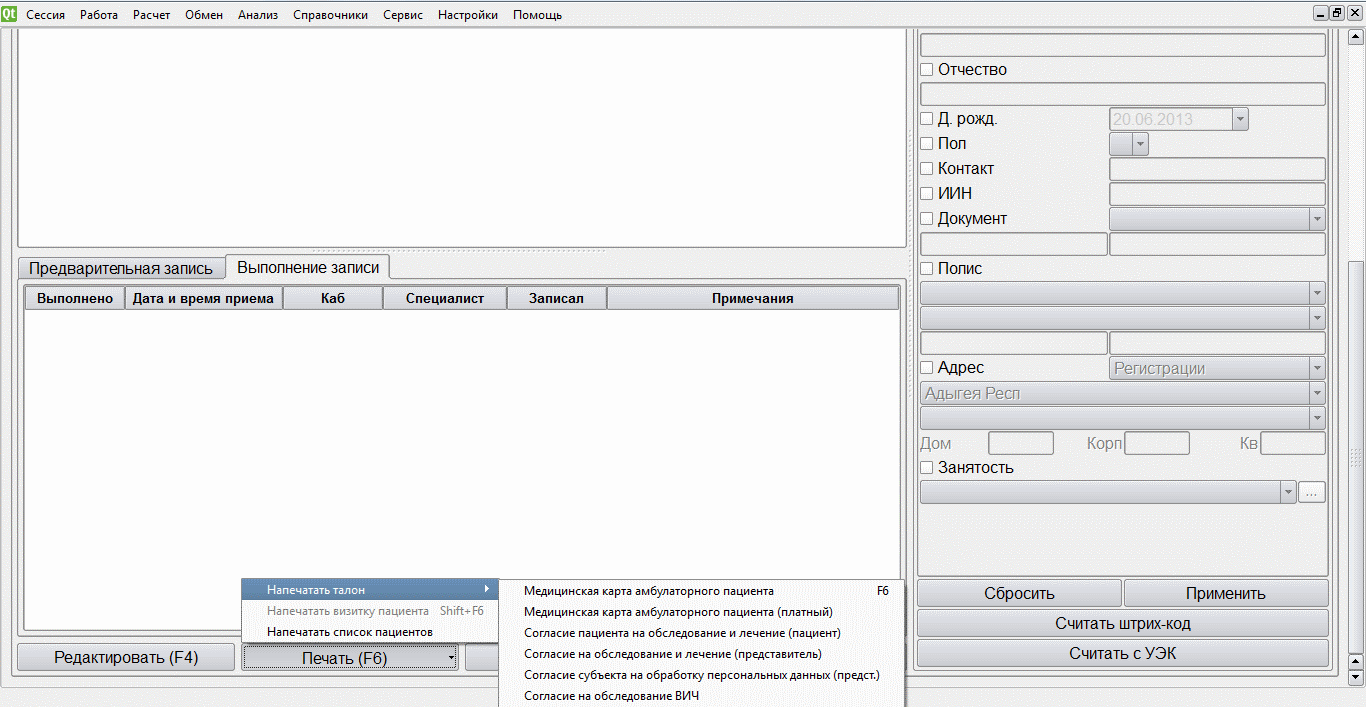
\includegraphics[width = 1\textwidth ,keepaspectratio]{cl_printm}
 \caption{Печать медицинских документов пациента}
 \label{img_cl_printm}
\end{figure} 

Кнопка \btn{Печать компактно} тоже выводит выбранные документы на печать, но не делает переход на новую страницу для каждого нового документа.

Если хотя бы для одного из выбранных для печати документов требуется указане параметров, то в правом нижнем углу всплывающего окна появится кнопка \btn{Далее} (кнопки \btn{Печать} и \btn{Печать компактно}) при этом будут недоступны, при натии на которую осуществляется переход в окно задания параметров формирования печатной формы. После заполнения параметров в данном окне можно нажать кнопку \btn{Печать} и \btn{Печать компактно}.

Печать документов пациента так же можно вызвать со страницы обслуживания пациентов (Рисунок \ref{img_cl_findrez}). Для этого необходимо найти пациента и щелкнуть по нему левой кнопкой мыши. В открывшемся окне (Рисунок \ref{img_cl_contrwin}) нужно нажать кнопку 
\includegraphics[scale=0.6]{print} в нижней части либо в правом верхнем углу окна. Откроется список документов для печати (Рисунок \ref{img_cl_printm}), где можно выбрать и вывести на печать документы вышеописанным способом. 
   
Печать медицинских документов, создаваемых в процессе обследования и лечения пациента, будет рассмотрена в следующих разделах.
}{}
 % 2. Картотека пациентов
  \newpage
\section{Работа поликлиники}

\subsection{Расписание работы врачей и квотирование}

\subsubsection{Создание расписания работы врачей}

Расписание работы врачей, ведущих амбулаторный прием, должно регулярно создаваться на последующий период работы ЛПУ в случае, если в ЛПУ организован прием пациентов по предварительной записи или по талонам. В зависимости от организации работы в конкретном ЛПУ, период, на который составляется расписание может быть различным. С целью минимизации трудозатрат на данную процедуру, рекомендуется создавать расписание на календарный месяц. Однако, возможно создание расписания и на более короткий (или более продолжительный) период.

Для создания расписания на новый период следует выбрать в главном меню пункт \mm{Работа \str Учет рабочего времени}. В открывшемся окне \dm{График} (Рисунок \ref{img_pol_shd}) необходимо:
\begin{enumerate}
 \item В секции 1 в верхней части календаря выбрать месяц года, на который требуется составить расписание, либо к которому относится период составления расписания.
 \item В секции 2 можно выбрать подразделение, для сотрудников которого составляется расписание. Тогда в секции 3 список будет ограничен только сотрудниками выбранного подразделения. По умолчанию курсор установлен на корневом элементе дерева структуры ЛПУ, в этом случае в секции 3 будет отображаться полный список сотрудников ЛПУ.
 \item В секции 3 установить курсор на записи о сотруднике, для которого необходимо составить расписание.
 \item Заполнить расписание сотрудника на требуемый период одним из следующих способов:
  \begin{itemize}
   	\item Заполнение расписания с помощью шаблона рассмотрено в п. \ref{pol_shdsh}
 	\item Заполнение расписания по шаблону «скользящий график» описано в п. \ref{pol_shdsg}
 	\item Заполнение расписания по персональному графику описано в п. \ref{pol_shdpers}
 	\item Копирование расписания с предыдущего месяца рассмотрено в п. \ref{pol_shdcopy}
  \end{itemize}	
\end{enumerate}

После того как расписание будет заполнено одним из вышеперечисленных способов, в секции 4 появится расписание выбранного врача, а в секции 5 будет выполнено подведение итогов по составленному расписанию врача.

\begin{figure}[ht]\centering
 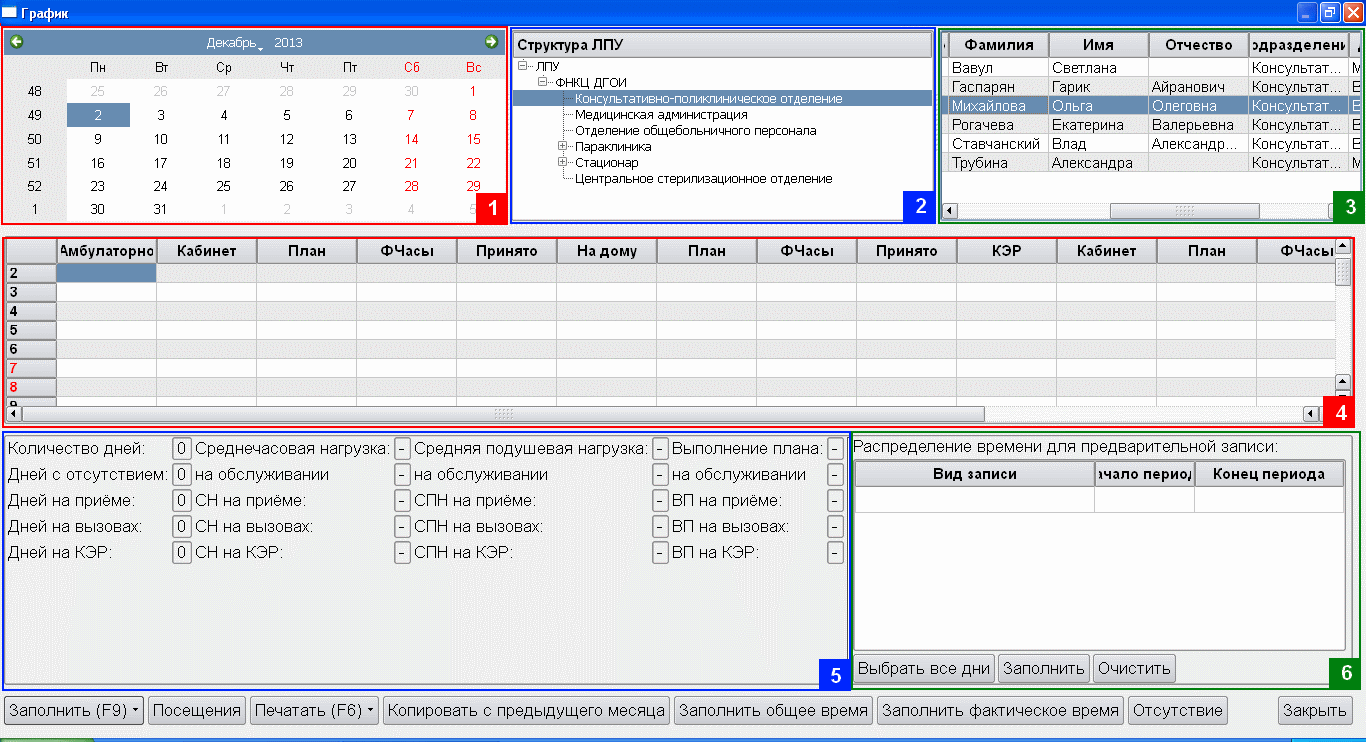
\includegraphics[width = 1\textwidth ,keepaspectratio]{pol_shd}
 \caption{Окно <<График>>}
 \label{img_pol_shd}
\end{figure}

Таблица, расположенная в секции 4 (Рисунок \ref{img_pol_shd}) имеет следующие столбцы:
\begin{itemize}
 \item В первом столбце таблицы указываются числа выбранного в секции 1 месяца. Т.е. каждому дню месяца соответствует одна строка в таблице расписания врача.
 \item \dm{Амбулаторно} – часы амбулаторного приема. Следующие за данным столбцом колонки относятся к часам амбулаторного приема;
 \begin{itemize}
  \item \dm{Кабинет} – кабинет амбулаторного приема;
  \item \dm{План} – плановое количество пациентов за амбулаторный прием;
  \item \dm{ФЧасы} – фактические часы амбулаторного приема;
  \item \dm{Принято} – фактическое количество обслуженных за время приема пациентов;
 \end{itemize} 
 \item \dm{На дому} – часы обслуживания вызовов на дом. Как и для амбулаторного приема, следующие за данным столбцом колонки относятся к часам вызовов на дом: \dm{План}, \dm{ФЧасы}, \dm{Принято}.
 \item \dm{КЭР} – часы выполнения клинико-экспертной работы. Далее, за этим столбцом идут колонки \dm{Кабинет}, \dm{План}, \dm{ФЧасы}, \dm{Принято}, относящиеся к часам клинико-экспертной работы.
 \item \dm{Прочее} – время, затрачиваемое на виды работ, не учтенные в расписании.
 \item \dm{Табель} – количество часов, учитываемое в табеле рабочего времени за указанный день.
 \item \dm{Причина отсутствия} – выбирается из списка в случае, если врач не проводил прием и обслуживание пациентов.
\end{itemize}
 
Часть ячеек данной таблицы заполняется с помощью шаблонов и других автоматизированных способов. Остальные ячейки можно заполнить вручную.

\paragraph{Составление расписания по шаблону} \label{pol_shdsh}

Данный вариант удобно использовать, если расписание работы врача подчиняется одной из следующих закономерностей:
\begin{itemize}
 \item Расписание одинаково на каждый день заданного периода;
 \item Расписание чередуется по четным и нечетным дням заданного периода;
 \item Имеется постоянное расписание работы на каждый из дней недели заданного периода.
\end{itemize}
 
\begin{figure}[ht]\centering
 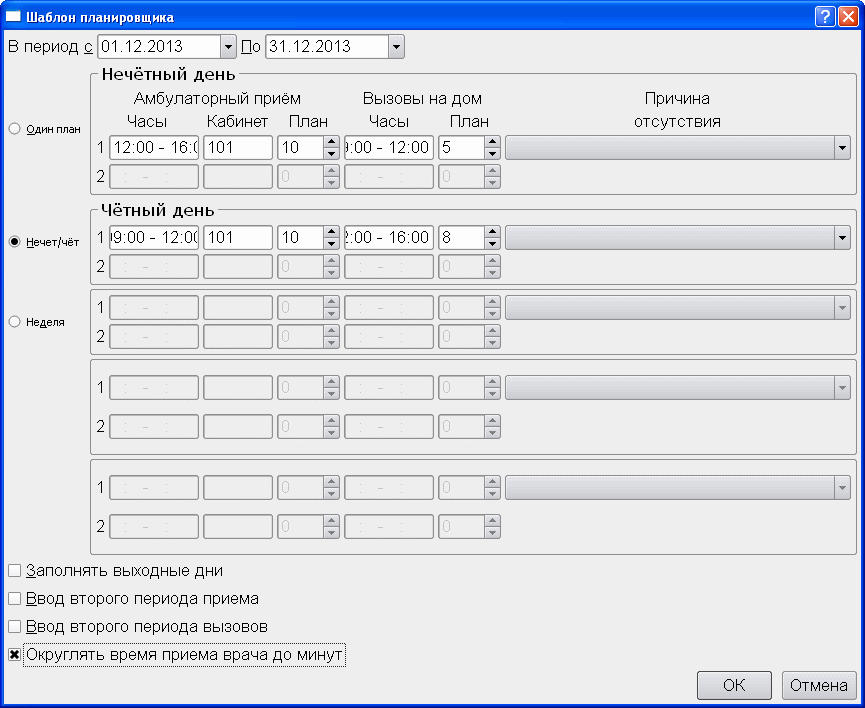
\includegraphics[width = 0.8\textwidth ,keepaspectratio]{pol_shdsh}
 \caption{Окно составления расписания по шаблону}
 \label{img_pol_shdsh}
\end{figure} 

Для использования этого варианта заполнения расписания необходимо после нажатия кнопки   в появившемся контекстном меню выбрать пункт \dm{По шаблону}. В открывшемся окне \dm{Шаблон планировщика} (Рисунок \ref{img_pol_shdsh}) следует:
\begin{itemize}
 \item В полях \dm{Период с} и \dm{По} ввести или выбрать из календаря период, на который необходимо составить расписание. По умолчанию в качестве периода указываются даты начала и окончания месяца, выбранного в секции 1 (Рисунок \ref{img_pol_shd}). Период составления расписания по шаблону не может выходить за границы этого месяца.
 \item Выбрать вид шаблона с помощью переключателя. В системе поддерживается 3 вида шаблонов расписания:
 \begin{itemize}
  \item \dm{Один план} – создается одинаковое расписание на все дни выбранного периода. Соответственно, только одна строка параметров расписания доступна для редактирования.
  \item \dm{Нечет\slash Чет} – будет предложено ввести 2 различных варианта расписания, первый из которых (в верхней строке) будет использоваться для нечетных дней месяца, а второй – для четных. 
  \item \dm{Неделя} – расписание создается отдельно для каждого дня недели с понедельника по пятницу.
 \end{itemize}	
 \item Заполнить каждую из активных строк расписания, указав следующие данные:
 \begin{itemize}
  \item \dm{Амбулаторный прием}: \dm{Часы} – часы амбулаторного приема, \dm{Кабинет} – номер кабинета, в котором ведется амбулаторный прием, \dm{План} – норма пациентов, которых следует принять за указанные часы.
  \item \dm{Вызовы на дом}: \dm{Часы} – часы обслуживания пациентов на дому, \dm{План} – норма пациентов, которых следует обслужить на дому за указанное время.
  \item \dm{Причина отсутствия}. Использование данного поля позволяет автоматизировать заполнение отсутствий сотрудников. При выборе причины отсутствия в какой-либо строке, расписание на соответствующие этой строке дни не заполняется, а только указывается причина отсутствия. Таким образом, если в строке указана причина отсутствия, то расписание в ней заполнять не нужно.
 \end{itemize} 
 Если в карточке сотрудника указан кабинет и/или плановое количество пациентов, то они будут подставлены в соответствующие поля шаблона автоматически. Данные значения можно изменить при необходимости.
 \item Установить флажок \dm{Заполнять выходные дни}, если расписание по выбранному шаблону следует так же создать на субботу и воскресенье. Данный флажок возможно использовать только с шаблонами \dm{Один план} и \dm{Нечет\slash Чет}.
 \item Установить флажок \dm{Ввод второго периода приема}, если время амбулаторного приема у врача разбито на 2 отдельных периода. После установки данного флажка для каждой строки расписания становится доступной вторая строка. В первой строке каждой группы необходимо ввести время, кабинет и норму приема для первого периода приема, а во второй – аналогичные данные для второго периода приема.
 \item Установить флажок \dm{Ввод второго периода вызовов}, если время обслуживания вызовов на дом у врача разбито на 2 отдельных периода. После установки данного флажка для каждой строки расписания становится доступной вторая строка. В первой строке каждой группы необходимо ввести время и норму обслуживания для первого периода вызовов на дом, а во второй – аналогичные данные для второго периода обслуживания вызовов.
 \item Установить флаг \dm{Округлять время приема врача до минут}, если НЕ нужно учитывать время с точностью до секунды при формировании талонов на прием.
 \item Нажать кнопку \btn{OK}  в правом нижнем углу окна. Текущее окно будет закрыто, а в секции 4 (Рисунок \ref{img_pol_shd}) появится заполненное расписание за период либо информация об отсутствиях сотрудника.
\end{itemize}

\begin{prim}
Если повторно выполнить формирование расписания по шаблону на период, на который ранее уже было создано расписание, то предыдущее расписание будет удалено полностью на указанный период, а затем будет создано новое расписание. Повторное формирование расписания возможно только в случае, если в указанном периоде нет занятых интервалов (номерков)   
\end{prim}

\paragraph{Составление расписания по шаблону «Скользящий график»} \label{pol_shdsg}

Данный вариант формирования расписания можно использовать, если не удалось выявить закономерности, описанные в предыдущем подразделе.

Для использования этого варианта заполнения расписания необходимо после нажатия кнопки \btn{Заполнить (F9)}  в появившемся меню выбрать пункт \dm{По шаблону <<скользящий график>>}. В открывшемся окне \dm{Шаблон планировщика} (Рисунок \ref{img_pol_shdsg}) следует:
\begin{itemize}
 \item Выбрать в календаре в центральной части окна дни месяца, в которые расписание работы врача одинаково. Выбор дней осуществляется однократным щелчком левой кнопки мыши по дате в календаре. При этом выбранные дни перечисляются через запятую справа от календаря в поле \dm{Выбранные дни}. Повторный щелчок левой кнопкой мыши по тому же дню в календаре исключает его из списка выбора. Для того чтобы удалить все дни из списка выбора необходимо нажать кнопку \btn{Очистить}. В данном окне доступны для выбора только дни месяца, который ранее был выбран в окне \dm{График} (Рисунок \ref{img_pol_shd}, секция 1).
 \item В верхней части окна заполнить расписание на выбранные дни либо причину отсутствия (аналогично описанному в п. \ref{pol_shdsh})
 \item Если необходимо, чтобы расписание заполнялось так же и на выходные дни, следует установить флажок \dm{Заполнять выходные дни}. Иначе выходные дни будут автоматически пропускаться при составлении расписания, даже если соответствующие даты включены в список выбора.
 \item При необходимости задания для выбранных дат второго периода амбулаторного приема либо второго периода обслуживания вызовов врача на дом, следует установить флажки \dm{Ввод второго периода приема} и \dm{Ввод второго периода вызовов} соответственно, а затем заполнить ставшие доступными поля настройки второго периода в верхней части окна (аналогично описанному в п. \ref{pol_shdsh})
 \item Установить флаг \dm{Округлять время приема врача до минут}, если не нужно учитывать время с точностью до секунды при формировании талонов на прием.
 \item Нажать кнопку \btn{OK} в правом нижнем углу окна. Текущее окно будет закрыто, а в секции 4 (Рисунок \ref{img_pol_shd}) появится заполненное расписание на ранее выбранные даты либо информация об отсутствиях сотрудника.
 \item Нужно повторить описанные действия для каждой группы дат в выбранном месяце, в которые расписание врача одинаковое.
\end{itemize}

\begin{figure}[ht]\centering
 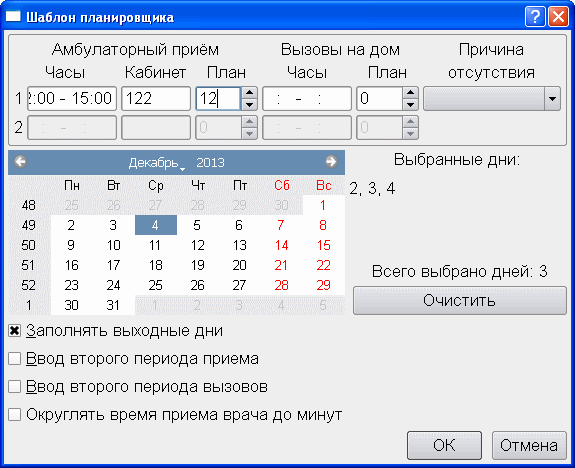
\includegraphics[width = 0.5\textwidth ,keepaspectratio]{pol_shdsg}
 \caption{Окно составления расписания по шаблону <<скользящий график>>}
 \label{img_pol_shdsg}
\end{figure} 

\begin{prim}
Если при формировании расписания была указана дата, на которую расписание уже заполнено, то расписание на эту дату будет полностью удалено, а затем заполнено в соответствии с новыми данными. Повторное формирование расписания на дату возможно только в случае, если на нее не записан ни один пациент 
\end{prim}

\paragraph{Составление расписания по персональному графику} \label{pol_shdpers}

Данный способ составления расписания удобно использовать, если сотрудник имеет постоянное расписание, которое не меняется от месяца к месяцу. Тогда можно настроить шаблон расписание врача в карточке сотрудника (\mm{Справочники \str Персонал \str Сотрудники}) на вкладке \dm{График} (Рисунок \ref{img_pol_shdpers}) и постоянно использовать его при создании расписания на новый период.

\begin{figure}[ht]\centering
 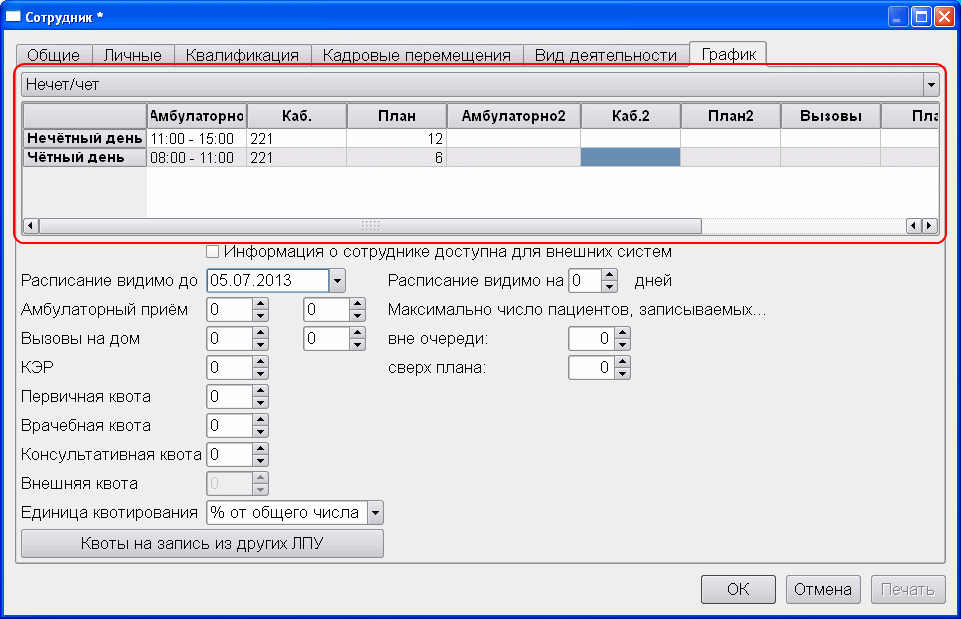
\includegraphics[width = 0.8\textwidth ,keepaspectratio]{pol_shdpers}
 \caption{Настройка расписания работы врача в карточке сотрудника}
 \label{img_pol_shdpers}
\end{figure} 

Для использования этого варианта заполнения расписания необходимо после нажатия кнопки \btn{Заполнить (F9)} в появившемся меню выбрать пункт \dm{По персональному графику}. В открывшемся окне \dm{Персональный шаблон} (Рисунок \ref{img_pol_shdpp}) нужно:
\begin{itemize}
 \item В полях \dm{В период с} и \dm{По} ввести или выбрать из календаря соответственно даты начала и окончания периода составления расписания.
 \item При необходимости установить флажок \dm{Заполнять выходные дни}. Если он установлен, то при составлении расписания будут заполняться выходные дни, при условии, что выходные дни заполнены в персональном шаблоне расписания врача. Если данный флажок снят, то расписание в выходные дни заполняться не будет вне зависимости от настроек расписания на выходные дни в персональном шаблоне расписания сотрудника.
 \item При необходимости установить флажки \dm{Ввод второго периода приема} и \dm{Ввод второго периода вызовов}. При установке данных флажков в расписание добавляются соответственно вторые периоды приема и вызовов, если они настроены в персональном шаблоне сотрудника. Если данные флажки сняты, то вторые периоды игнорируются даже при наличии соответствующих настроек в персональном шаблоне сотрудника. Флажки \dm{Ввод второго периода приема} и \dm{Ввод второго периода вызовов} можно использовать как совместно, так и отдельно друг от друга.
 \item Установить флаг \dm{Округлять время приема врача до минут}, если НЕ нужно учитывать время с точностью до секунды при формировании талонов на прием.
 \item Нажать кнопку \btn{OK} в правом нижнем углу окна. Текущее окно будет закрыто, а в секции 4 (Рисунок \ref{img_pol_shd}) появится заполненное расписание сотрудника по его персональному шаблону.
\end{itemize}

\begin{figure}[ht]\centering
 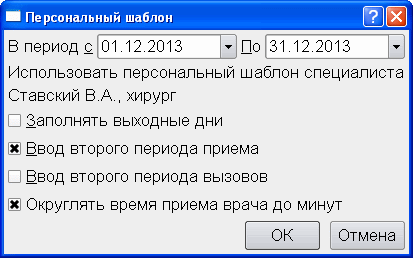
\includegraphics[width = 0.5\textwidth ,keepaspectratio]{pol_shdpp}
 \caption{Составление расписания по персональному шаблону}
 \label{img_pol_shdpp}
\end{figure}

\paragraph{Копирование расписания с предыдущего периода} \label{pol_shdcopy}

Если расписание сотрудника на текущий месяц аналогично его расписанию на предыдущий месяц, то можно скопировать расписание с предыдущего периода. Для этого нужно нажать кнопку \btn{Копировать с предыдущего периода} и в открывшемся окне (Рисунок \ref{img_pol_shdcopy}) установить следующие параметры:
\begin{itemize}
 \item По умолчанию копирование производится с начала предыдущего месяца. Для того чтобы изменить стартовую дату копирования, следует установить флаг начать с и в ставшем активным поле даты выбрать дату, которая должна быть точкой отсчета при копировании расписания.
 \item Если вместе с расписанием нужно скопировать настройки квотирования (см. п. \ref{pol_shdkv}) по времени с предыдущего периода, то следует установить флажок \dm{так же копировать квотирование по времени}.
 \item Выбрать один из режимов копирования:
 \begin{itemize}
  \item \dm{Один план} – на каждый день месяца будет скопировано расписание из ячейки, которая выбрана в качестве стартовой для копирования расписания.
  \item \dm{Нечет\slash Чет} – расписание будет скопировано с учетом различия настроек для четных и нечетных дней. Настройки расписания для четных дней предыдущего месяца будут скопированы на четные дни текущего месяца, а настройки расписания для нечетных дней предыдущего месяца будут скопированы на нечетные дни текущего месяца.
  \item \dm{Неделя} – расписание с каждого дня недели предыдущего месяца будет скопировано на соответствующие дни недели текущего месяца.
 \end{itemize}	
 \item Нажать кнопку \btn{OK}  в правом нижнем углу окна. Текущее окно будет закрыто, а в секции 4 (Рисунок \ref{img_pol_shd}) появится заполненное расписание на новый месяц.
\end{itemize}

\begin{figure}[ht]\centering
 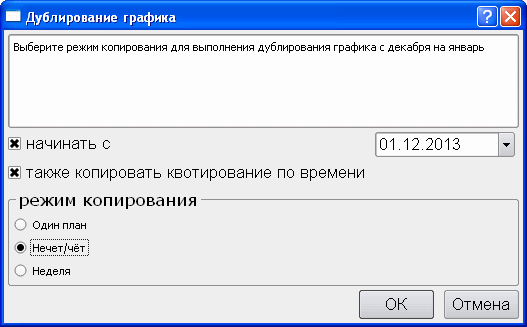
\includegraphics[width = 0.6\textwidth ,keepaspectratio]{pol_shdcopy}
 \caption{Копирование расписания с предыдущего месяца}
 \label{img_pol_shdcopy}
\end{figure}

\begin{prim}
 Если в целевом месяце (на который планируется скопировать расписание) у выбранного врача зарегистрирована хотя бы одна запись пациента на прием, копирование расписания становится невозможным 
\end{prim}

\subsubsection{Квотирование} \label{pol_shdkv}

Настройка квотирования для созданного расписания позволяет разделить весь период амбулаторного приема на интервалы времени, каждый из которых доступен для одного или нескольких из перечисленных видов записи:
\begin{itemize}
 \item Запись из регистратуры (к любому врачу);
 \item Запись врачом на повторный прием (к себе);
 \item Межкабинетная запись (запись врачом на консультацию к другим специалистам);
 \item Запись из других ЛПУ;
 \item Запись через Портал. 
\end{itemize}
 
Возможно так же распределение талонов на амбулаторный прием в процентном или числовом отношении между описанными видами записи.

\paragraph{Квотирование по времени}

Настройка квотирования талонов по времени приема выполняется из пункта меню \mm{Работа \str Учет рабочего времени} (Рисунок \ref{img_pol_shd}). Настройка квотирования осуществляется после того, как создано расписание врача на выбранный период. Для настройки квотирования по времени нужно:
\begin{itemize}
 \item В расписании сотрудника (секция 4, Рисунок \ref{img_pol_shd}) выделить с помощью мыши один или несколько дней, для которых следует распределить талоны. В выделение должны попадать дни с одинаковыми часами приема. Идущие подряд дни можно выделить, нажав левую кнопку мыши на первой строке интервала и удерживая ее до тех пор, пока указатель мыши не будет перемещен на последнюю строку интервала. Выделить несколько не подряд идущих строк можно, щелкая по соответствующим ячейкам правой кнопкой мыши при нажатой клавише \keys{Ctrl} на клавиатуре. Для выделения всех дней, на которые есть расписание в выбранном месяце, можно нажать кнопку \btn{Выбрать все дни}  в правом нижнем углу окна (секция 6, Рисунок \ref{img_pol_shd}).
\end{itemize}

\begin{prim}
 Если требуется, чтобы в выделение попала большая часть строк, можно нажать кнопку \btn{Выбрать все дни}, я затем щелкнуть по ячейкам, которые необходимо исключить из выделения, правой кнопкой мыши при нажатой клавише \keys{Ctrl} на клавиатуре. Аналогичным способом можно исключить ошибочно добавленные ячейки из любого выделения.
\end{prim}

\begin{itemize}
 \item В таблице \dm{Распределение времени для предварительной записи} (секция 6, Рисунок \ref{img_pol_shd}) настроить квотирование по времени для выбранных дней. Для этого в строках таблицы нужно выбрать из списка вид записи и указать для нее время начала и окончания периода времени, в который доступен выбранный вид записи. Активация новой строки производиться двойным щелчком левой кнопки мыши по любой из ячеек этой строки. Можно добавить несколько видов записи на один день. Допускается добавление нескольких периодов одного вида в один день. Периоды времени для разных видов записи в рамках одного дня могут пересекаться, тогда данное время будет доступно сразу для двух или нескольких видов записи. Периоды времени квотирования по различным видам записи не должны выходить за границы общего времени амбулаторного приема.
 \item После того как квотирование по времени для выбранных дней настроено, нажать кнопку \btn{Заполнить}. Если в таблице \dm{Распределение времени для предварительной записи} имеются записи, время которых выходит за границы общего времени амбулаторного приема, на экране появится соответствующее предупреждение. Если ошибок не обнаружено, то заполнение интервалов квотирования для выбранных дней произойдет без дополнительных оповещений.
\end{itemize}
 
Описанные выше шаги следует повторить столько раз, сколько потребуется для настройки квотирования для каждого из дней амбулаторного приема сотрудника.

При записи пациентов на прием интервалы, которые недоступны для записи текущему пользователю, будут окрашены в темно-серый цвет (Рисунок \ref{img_pol_kvot}). При попытке записать пациента на такой интервал времени, будет выдано сообщение о невозможности записи.

\begin{figure}[ht]\centering
 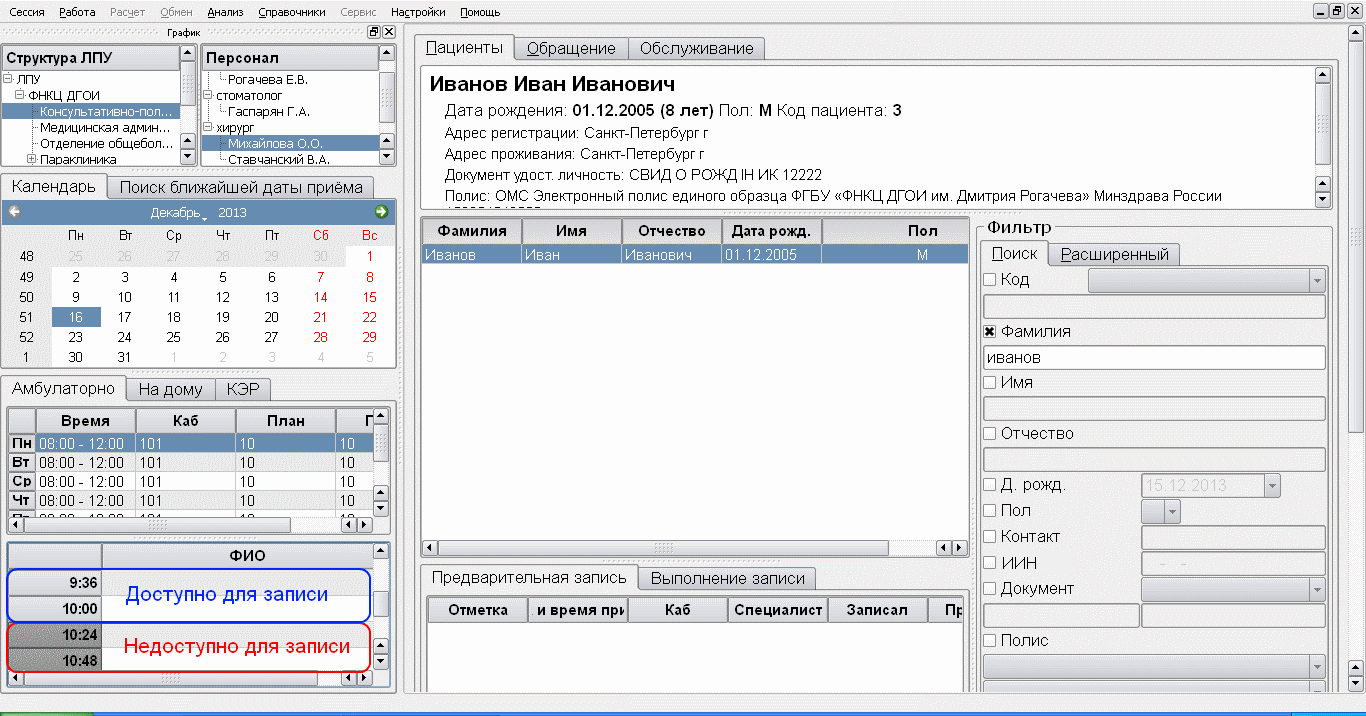
\includegraphics[width = 1\textwidth ,keepaspectratio]{pol_kvot}
 \caption{Доступные интервалы записи на прием}
 \label{img_pol_kvot}
\end{figure}

При выборе какой-либо из строк расписания (секция 4, Рисунок \ref{img_pol_shd}) в таблице \dm{Распределение времени для предварительной записи} должно отображаться квотирование по времени для выбранного дня. Если выделено сразу несколько строк в расписании сотрудника, то распределение времени по ним будет отображаться только в том случае, если оно совпадает для всех выбранных строк.

Если в результате вышеописанного группового выбора будет настроен и заполнен новый вариант квотирование, то предыдущие настройки квотирования по времени будут удалены для выбранных дней.

\begin{vnim}
Если в настройках квотирования часть времени амбулаторного приема оказалась не распределенной ни на один из видов записи, то это время будет доступно для всех видов записи.
\end{vnim}
 
\begin{prim}
 Если в настройках квотирования отсутствует какой-либо вид записи, то для него возможна запись на любой интервал времени амбулаторного приема на выбранный день. Для того чтобы запретить какой-либо вид записи на определенные дни, нужно добавить его в таблицу \dm{Распределение времени для предварительной записи} и указать в качестве интервала какой-либо несуществующий интервал.
\end{prim}

Для удаления настройки квотирования по времени на какой-либо день или несколько дней следует выделить их в расписании сотрудника, а затем нажать кнопку \btn{Очистить}  в правом нижнем углу окна.

\begin{vnim}
 При отсутствии настроек квотирования по времени вступают в силу настройки квотирования по количеству талонов, указанные в карточке сотрудника.
\end{vnim}

\paragraph{Квотирование по количеству талонов}

Квотирование по количеству талонов используется, если для выбранного дня отсутствуют настройки квотирования по времени. Квотирование по количеству талонов может задаваться в абсолютном или процентном соотношении и настраивается в карточке сотрудника (\mm{Справочники \str Персонал \str Сотрудники}) на вкладке \dm{График} (Рисунок \ref{img_pol_shdpers}) в нижней части окна.
\begin{itemize}
 \item В строке \dm{Амбулаторный прием} следует указать плановое количество пациентов, которых врач должен обслужить за один прием. От этого количества будут рассчитываться квоты для различных видов записей. Здесь предусмотрено 2 поля. Во втором поле указывается плановое количество пациентов для второго периода приема (если он есть).
 \item В поле \dm{Первичная квота} указывается количество или процент талонов, доступных для записи из регистратуры.
 \item В поле \dm{Врачебная квота} указывается количество или процент талонов, доступных врачу для записи пациентов к себе на повторный прием.
 \item В поле \dm{Консультативная квота} указывается количество или процент талонов, доступных врачу для записи пациентов на консультации к другим специалистам (межкабинетная запись).
 \item Поле \dm{Внешняя квота} становится доступным только при установке флага \dm{Информация о сотруднике доступна для внешних систем}. В данном поле указывается количество или процент талонов, доступных для записи из других ЛПУ и через Портал.
 \item В поле \dm{Единица квотирования} выбирается значение из списка. Если выбрано <<абсолютное число>>, то во всех вышеописанных полях нужно указывать количество доступных талонов. При этом суммарное число талонов по всем видам квот должно равняться значению в поле \dm{Амбулаторный прием}. Если выбрано значение <<\% от общего числа>>, то во всех вышеописанных полях нужно указывать процент от общего числа талонов, доступных для соответствующего вида записи. При этом суммарное значение всех квот должно составлять 100\%.
\end{itemize}

В карточке сотрудника так же можно ограничить число талонов, доступных для каждого из внешних ЛПУ. Устанавливается месячная квота общая для всех врачей ЛПУ указанной специальности. Для включения этого механизма квотирования следует нажать кнопку \btn{Квота на запись из других ЛПУ} и в открывшемся окне (Рисунок \ref{img_pol_kvotlpu}) установить флаг \dm{Включить квотирование}. Если таблица квотирования пуста, то необходимо заполнить ее, выбирая внешнее ЛПУ из справочника и указывая месячный лимит талонов по данной специальности. После заполнения таблицы необходимо нажать кнопку \btn{Сохранить}.

\begin{figure}[ht]\centering
 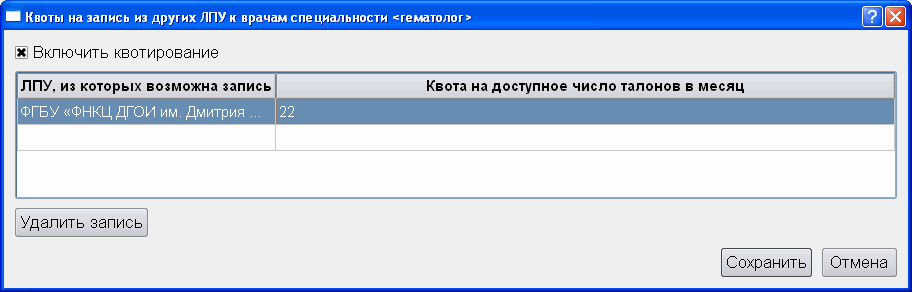
\includegraphics[width = 1\textwidth ,keepaspectratio]{pol_kvotlpu}
 \caption{Квотирование числа талонов для внешних ЛПУ}
 \label{img_pol_kvotlpu}
\end{figure}

Для редактирования заполненных полей таблицы, нужно дважды щелкнуть левой кнопкой мыши по нужной ячейке и ввести новое значение. После внесения изменений необходимо нажать кнопку \btn{Сохранить}.

Для удаления строки из таблицы квотирования для внешних ЛПУ нужно установить курсор на строку, подлежащую удалению и нажать кнопку \btn{Удалить запись} в левом нижнем углу окна. После удаления строк, необходимо сохранить сделанные изменения кнопкой \btn{Сохранить}.

\subsubsection{Возможности использования групповых операций при создании расписания}

При составлении и редактировании расписания из пункта меню \mm{Работа \str Учет рабочего времени} ряд операций может выполняться для нескольких врачей одновременно. Операции сразу над несколькими записями называются групповыми. Для выполнения групповых операций необходимо в секции 3 (Рисунок \ref{img_pol_shd}) выбрать сразу несколько врачей, используя выделение мышью, если записи расположены подряд, либо щелкая по нужным записям левой кнопкой мыши при нажатой клавише \keys{Ctrl} на клавиатуре, для не подряд идущих записей. Для выделения всех строк, находящихся в секции 3 (Рисунок \ref{img_pol_shd}) на текущий момент можно щелкнуть правой кнопкой мыши на любой строке и в появившемся контекстном меню выбрать пункт \dm{Выделить все строки}. Для снятия выделения можно щелкнуть левой кнопкой мыши в любом месте списка сотрудников (секция 3, Рисунок \ref{img_pol_shd}) либо щелкнуть правой кнопкой мыши по одной из строк таблицы и в появившемся контекстном меню выбрать пункт \dm{Снять выделение}.

Для выделенных записей доступны следующие групповые операции:
\begin{enumerate}
 \item Составление расписания по шаблону.
 \item Составление расписания по персональному графику.
 \item Изменение параметров доступа к расписанию выбранных врачей.
 \item Изменение доступности расписания выбранных врачей для внешних систем.
\end{enumerate}

\paragraph{Составление расписания по шаблону для нескольких сотрудников}

Данную операцию можно применить, если несколько сотрудников имеют идентичное расписание на выбранный период. Для выполнения операции необходимо:
\begin{enumerate}
 \item Выделить несколько записей о сотрудниках (см. выше).
 \item Нажать кнопку \btn{Заполнить(F9)}  в левом нижнем углу окна и в появившемся меню выбрать пункт \dm{По шаблону}.
 \item В открывшемся окне указать параметры расписания аналогично тому, как это делалось при создании расписания одного сотрудника (см. п. \ref{pol_shdsh}) и нажать кнопку \btn{OK} .
 \item Появится окно \dm{Массовое добавление графиков на специалистов}, показывающее ход процесса формирования расписания (Рисунок \ref{img_pol_pubshd}). После того как в окне отобразится состояние выполнения 100\% (ГОТОВО), нужно закрыть текущее окно. Расписание сформировано.
\end{enumerate}

\begin{figure}[ht]\centering
 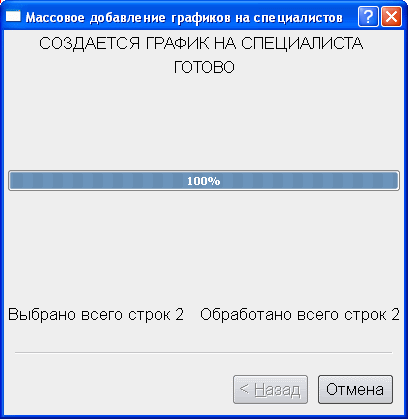
\includegraphics[width = 0.5\textwidth ,keepaspectratio]{pol_pubshd}
 \caption{Ход процесса группового создания расписания}
 \label{img_pol_pubshd}
\end{figure} 
 
\begin{vnim}
 После завершения формирования расписания групповое выделение с записей о сотрудниках снимается автоматически.
\end{vnim}

\paragraph{Составление расписания по персональному графику для нескольких сотрудников}

Данную операцию можно применить, если для всех или нескольких сотрудников имеются настройки расписания работы на вкладке \dm{График} карточки сотрудника.

Для выполнения операции необходимо:
\begin{enumerate}
 \item Выделить несколько записей о сотрудниках (см. выше).
 \item Нажать кнопку \btn{Заполнить(F9)}  в левом нижнем углу окна и в появившемся меню выбрать пункт \dm{По персональному графику}.
 \item Появится окно \dm{Массовое добавление графиков на специалистов}, показывающее ход процесса формирования расписания (Рисунок \ref{img_pol_pubshd}). После того как в окне отобразится состояние выполнения 100\% (ГОТОВО), нужно закрыть текущее окно. Расписание сформировано.
\end{enumerate}
 
\begin{vnim}
 После завершения формирования расписания групповое выделение с записей о сотрудниках снимается автоматически.
\end{vnim}

\paragraph{Изменение параметров доступа к расписанию выбранных врачей}

Данная операция позволяет изменить время, с которого расписание становится доступным для записи, задаваемое в карточке сотрудника. Для выполнения данной операции необходимо:
\begin{enumerate}
 \item Выделить все или несколько записей о сотрудниках (см. выше).
 \item Щелкнуть правой кнопкой мыши по одной из выделенных строк и в появившемся контекстном меню выбрать пункт \dm{Изменить параметры доступа к расписанию}.
 \item В открывшемся окне (Рисунок \ref{img_pol_pubshd2}) установить флажок справа от поля \dm{Расписание видимо до} и указать дату, до которой расписание должно быть доступно для записи, либо установить флажок \dm{Расписание видимо на} и указать количество дней, на которые расписание доступно относительно текущей даты.
 \item Нажать кнопку \btn{OK}.
 \item Изменения будут внесены в карточку сотрудника, что сразу же отразится в ячейках \dm{Расписание видимо до} и \dm{Расписание видимо на} для выделенных строк секции 4 (Рисунок \ref{img_pol_shd}).
\end{enumerate}

\begin{figure}[ht]\centering
 
\includegraphics[width = 0.5\textwidth ,keepaspectratio]{pol_pubshd2}
 \caption{Изменение параметров доступа к расписанию}
 \label{img_pol_pubshd2}
\end{figure}  
 
\paragraph{Изменение доступности расписания выбранных врачей для внешних систем}

Данная операция позволяет изменить доступность расписания выбранных сотрудников для записи из других ЛПУ и через Портал. Для выполнения данной операции необходимо:
\begin{enumerate}
 \item Выделить все или несколько записей о сотрудниках (см. выше).
 \item Щелкнуть правой кнопкой мыши по одной из выделенных строк и в появившемся контекстном меню выбрать пункт \dm{Сделать доступным для внешних систем}, если расписание должно быть доступно, или \dm{Сделать недоступным для внешних систем}, если расписание должно быть недоступным соответственно.
 \item Изменения будут внесены в карточку сотрудника, что сразу же отразится в ячейке \dm{Доступ для ВС} для выделенных строк секции 4 (Рисунок \ref{img_pol_shd}).
\end{enumerate}

\subsection{Предварительная запись на прием}

Предварительная запись пациентов на прием осуществляется в окне картотеки пациентов. Для открытия данного окна в главном меню нужно выбрать пункт \mm{Работа \str Обслуживание пациентов}. Запись пациентов осуществляется на вкладке \dm{Картотека}.
Существует 2 способа записи пациентов на прием:
\begin{itemize}
 \item с помощью панели \dm{Графики};
 \item с помощью панели \dm{Номерки}.
\end{itemize}

\subsubsection{Запись на прием с использованием графика}

Для записи с помощью панели \dm{Графики}, должно быть включено отображение этой панели (Рисунок \ref{img_pol_zapgr}, секции 1 – 5). Если указанная панель отсутствует, ее нужно подключить в главном меню \mm{Настройки \str График}. После подключения в меню перед пунктом \dm{График} должен появиться установленный флажок \putx, а в левой части экрана соответствующая панель. Размеры отдельных секций панели можно регулировать с помощью мышки.

\begin{figure}[ht]\centering
 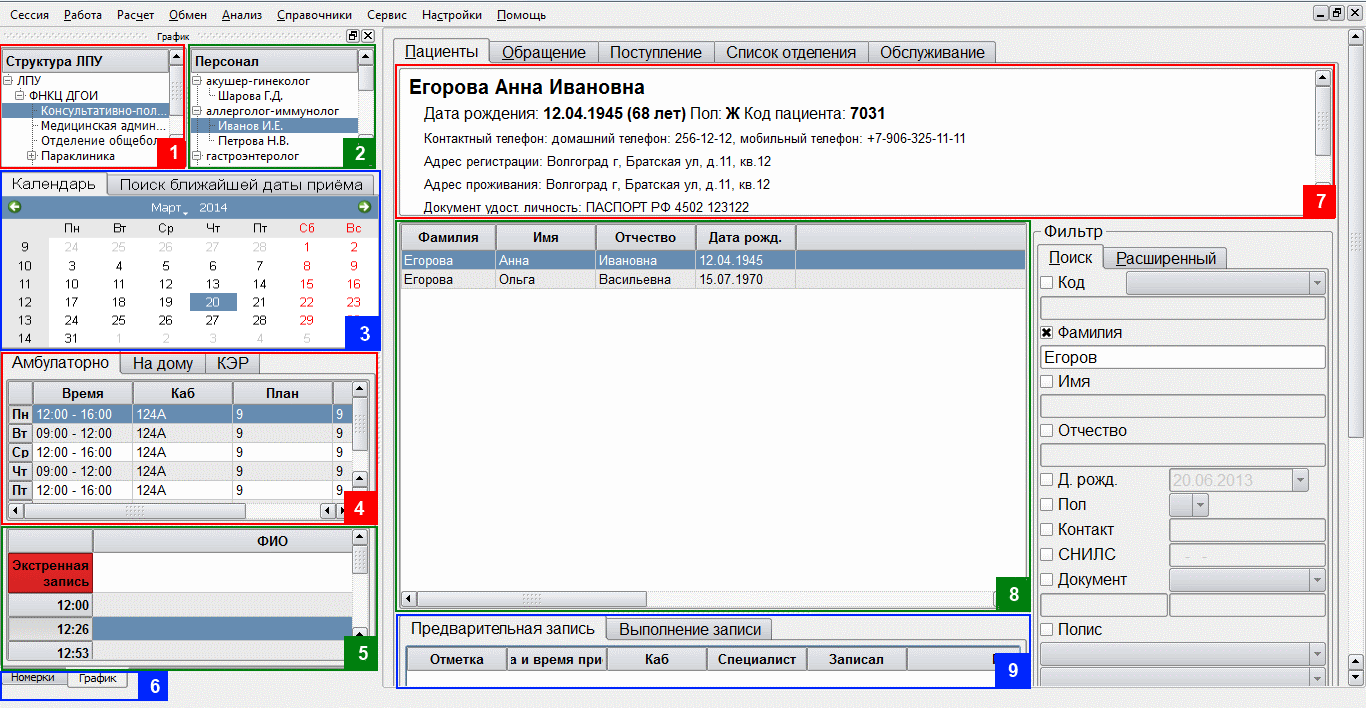
\includegraphics[width = 1\textwidth ,keepaspectratio]{pol_zapgr}
 \caption{Предварительная запись на прием по графику}
 \label{img_pol_zapgr}
\end{figure}  

Последовательность действий при записи пациента на прием должна быть следующая:
\begin{enumerate}
 \item С помощью фильтра или любым другим способом нужно найти пациента в картотеке и установить курсор в секции 8 на его имени так, чтобы в секции 7 отображалась краткая информация о выбранном пациенте. Если пациент не был зарегистрирован ранее, его следует зарегистрировать в картотеке пациентов.
 \item В секции 1 необходимо выбрать подразделение ЛПУ, куда требуется записать пациента, раскрывая соответствующие ветви дерева, нажатием значка <<$+$>> слева от названия подразделения.
 \item В секции 2 следует найти специальность врача и, раскрыв список нажатием кнопки <<$+$>> слева от названия специальности, установить курсор на фамилии специалиста, к которому нужно записать пациент.
 \item В секции 3 на вкладке \dm{Календарь} необходимо выбрать дату приема, щелкнув по ней левой кнопкой мыши. Перемещение на следующий месяц можно выполнить нажатием кнопки с изображением стрелки вправо в правом верхнем углу секции.
 \item После выбора даты курсор в секции 4 будет автоматически установлен на дне недели, соответствующем выбранной дате. В секции 4 отображается расписание работы врача на неделю.
 \item В секции 5 будет отображен список интервалов времени для записи на прием. В случае наличия свободного интервала нужно согласовать время с пациентом, щелкнуть по соответствующему интервалу в секции 5 правой кнопкой мыши и в появившемся меню выбрать \dm{Поставить в очередь}. При отсутствии свободных интервалов, подходящих пациенту, необходимо повторить шаги 4-6, выбрав другую дату.
 \item Если пациент записан на прием успешно, то в поле \dm{ФИО} выбранного интервала появятся данные пациента. В секции 9 для этого пациента на вкладке \dm{Предварительная запись} так же добавится новая строка о предварительной записи к выбранному врачу. На экране появится окно просмотра печатной формы направления. Для печати направления нужно нажать кнопку \btn{Печатать}, для сохранения направления в файл – кнопку \btn{Сохранить}. Если печать направления не требуется, то следует нажать кнопку \btn{Закрыть}.
\end{enumerate}
  
\begin{prim}
 При наличии соответствующей настройки, можно выполнять постановку пациента в очередь двойным щелчком левой кнопки мыши на соответствующем интервале.
\end{prim}
 
В \tmis~реализована возможность экстренной записи и записи сверх нормы на выбранную дату. Для записи экстренного пациента, нужно щелкнуть правой кнопкой мыши по первой строке секции 5 (Экстренная запись) и выбрать в меню \dm{Поставить в очередь}. Для записи пациентов сверх нормы следует щелкнуть правой кнопкой мыши по последней записи в секции 5 (Сверх очереди) и в контекстном меню выбрать пункт \dm{Поставить в очередь}. Возможность записи дополнительных пациентов и их количество настраивается для каждого врача отдельно. Если для врача запрещена запись дополнительных пациентов или количество дополнительных пациентов, записанных на выбранную дату, достигло максимального предела, при попытке записать еще одного пациента будет выдаваться сообщение <<Запись невозможна. Вы достигли квоты по записи сверх плана>>.

После записи пациента можно дополнительно указать жалобы или примечания для врача. Для этого нужно щелкнуть по интервалу с именем записанного пациента в секции 5 правой кнопкой мыши и в появившемся меню выбрать \dm{Изменить жалобы\slash примечания}. Данное действие так же можно выполнить, щелкнув по соответствующей записи на вкладке \dm{Предварительная запись} секции 9, и выбрав в меню пункт \dm{Изменить жалобы\slash примечания}.

Для повторной печати направления следует щелкнуть по соответствующей записи в секции 5 или 9 правой кнопкой мыши и в появившемся контекстном меню выбрать пункт \dm{Напечатать направление}.

Для отмены предварительной записи нужно щелкнуть по соответствующей строке в секции 5 или 9 правой кнопкой мыши и в появившемся контекстном меню выбрать пункт \dm{Удалить из очереди}, после чего подтвердить удаление записи, нажав кнопку \btn{OK}  в открывшемся диалоговом окне. Вне зависимости от способа выполнения действия, запись будет удалена из секции 9, а в секции 5 интервал будет освобожден.

\subsubsection{Поиск ближайшей даты приема специалиста}

В \tmis~реализована возможность поиска ближайшей даты приема специалиста, на которую есть свободные интервалы. 

Для поиска ближайшей даты приема необходимо:
\begin{itemize}
 \item В секции 3 (Рисунок \ref{img_pol_zapgr}) перейти на вкладку \dm{Поиск ближайшей даты приема}.
 \item В поле \dm{Специальность} выбрать из раскрывающегося списка нужную специальность врача и нажать кнопку \btn{Поиск} (Рисунок \ref{img_pol_zapfind}).
\end{itemize}

\begin{figure}[ht]\centering
 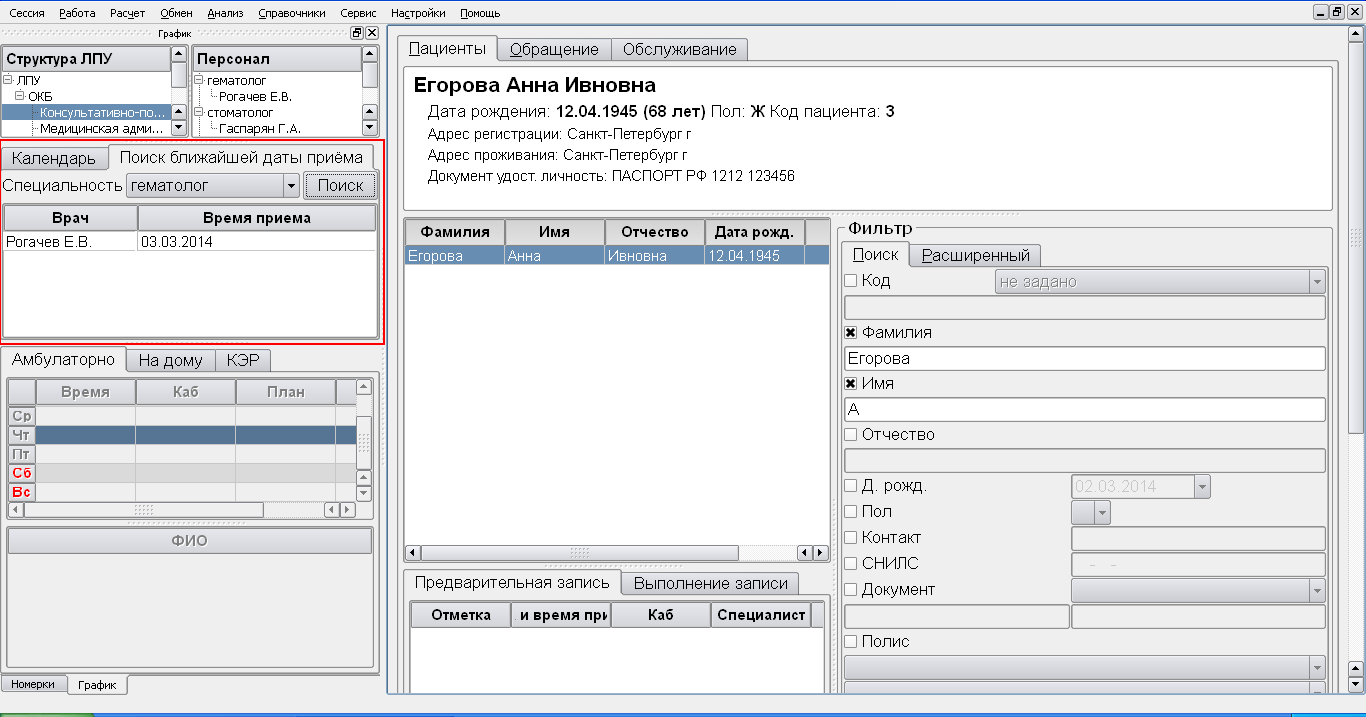
\includegraphics[width = 1\textwidth ,keepaspectratio]{pol_zapfind}
 \caption{Поиск ближайшей даты приема специалиста}
 \label{img_pol_zapfind}
\end{figure}

В результате поиска в таблице, расположенной под полем выбора специальности появится список врачей выбранной специальности, ведущих прием в ЛПУ. В поле \dm{Дата} будет указана ближайшая дата, доступная для записи. Если свободные номерки у врача отсутствуют, то в поле \dm{Дата} будет указано <<Нет талонов>>.

\subsubsection{Запись на прием с использованием номерков}

Для записи с помощью панели \dm{Номерки}, должно быть включено отображение этой панели (Рисунок \ref{img_pol_zapn}). Если указанная панель отсутствует, ее нужно подключить в главном меню \mm{Настройки \str Номерки}. После подключения в меню перед пунктом \dm{Номерки} должен появиться установленный флажок \putx, а в левой части экрана соответствующая панель. Размеры отдельных секций панели можно регулировать с помощью мышки. Если панели \dm{График} и \dm{Номерки} включены одновременно, то они организованы в виде вкладок. Переключение между вкладками осуществляется в нижней части панели (секция 5).

\begin{figure}[ht]\centering
 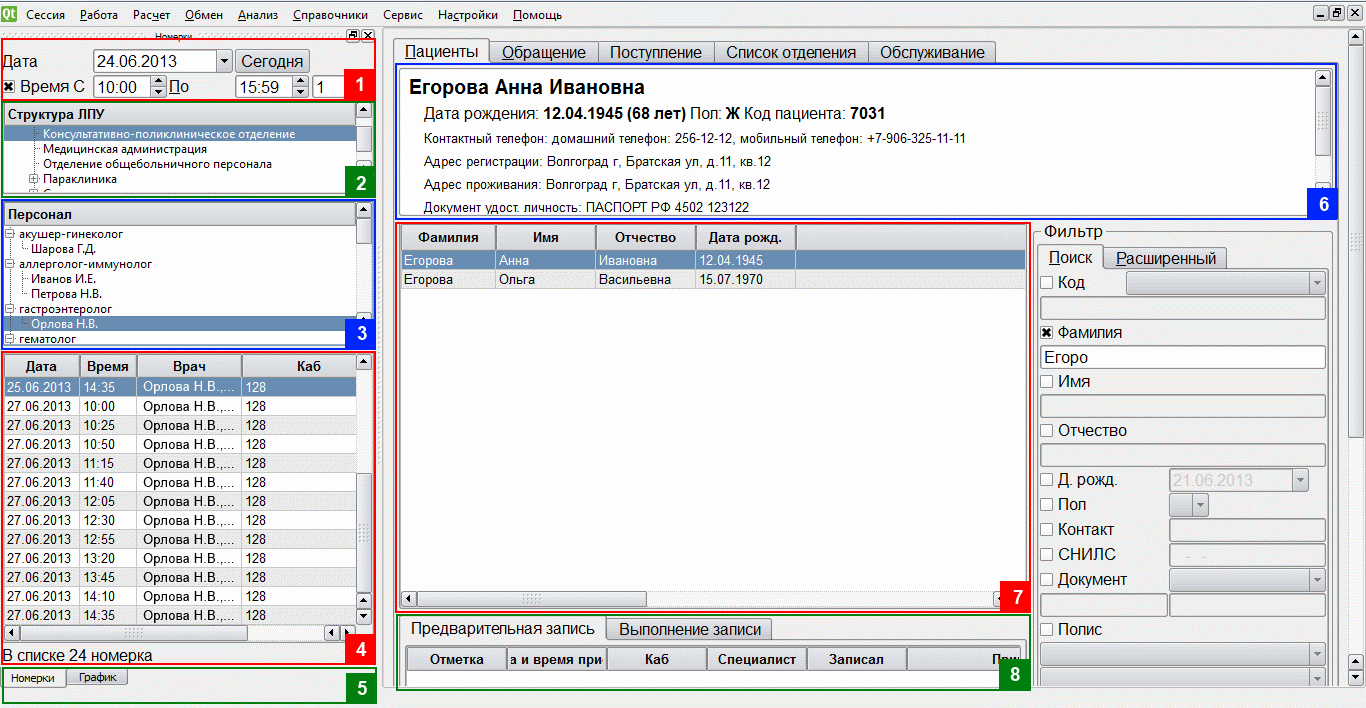
\includegraphics[width = 1\textwidth ,keepaspectratio]{pol_zapn}
 \caption{Предварительная запись на прием по номеркам}
 \label{img_pol_zapn}
\end{figure}  

Последовательность действий при записи пациента на прием с использованием номерков должна быть следующая:
\begin{enumerate}
 \item С помощью фильтра или любым другим способом необходимо найти пациента в картотеке и установить курсор в секции 7 на его имени так, чтобы в секции 6 отображалась краткая информация о выбранном пациенте. Если пациент не был зарегистрирован ранее, его следует зарегистрировать в картотеке пациентов.
 \item В секции 1 можно установить фильтр по дате и времени номерка. В поле \dm{Дата} нужно указать дату, начиная с которой следует вести поиск свободных номерков, в полях \dm{Время С} и \dm{По} можно указать желаемый период времени приема, в последнем поле можно указать требуемое количество идущих подряд свободных номерков. По умолчанию поиск свободных номерков осуществляется, начиная с текущей даты на любое время. При нажатии кнопки \btn{Сегодня}  в поле \dm{Дата} устанавливается текущая дата, если ранее она была изменена на иную.
 \item В секции 2 желательно выбрать подразделение ЛПУ, куда требуется записать пациента, раскрывая соответствующие ветви дерева, нажатием значка <<$+$>> слева от названия подразделения.
 \item В секции 3 нужно выбрать специальность врача или фамилию врача. Список врачей каждой специальности можно раскрыть, щелкнув левой кнопкой мыши по значку <<$+$>> слева от названия специальности.
 \item В секции 4 требуется выбрать подходящий номерок и щелкнув правой кнопкой мыши на нем, выбрать в появившемся меню пункт \dm{Поставить в очередь}. В результате этих действий номерок исчезнет из списка, а в секции 8 для выбранного пациента будет добавлена новая строка о предварительной записи.
\end{enumerate}
 
  
\begin{prim}
 При наличии соответствующей настройки, можно выполнять выдачу пациенту номерка двойным щелчком левой кнопки мыши на номерке.
\end{prim}
 
При записи на прием с использованием номерков существует так же возможность бронирования номерков. Для этого на шаге 5 нужно выбрать пункт меню \dm{Выполнить бронирование}. Номерок при этом останется в списке, но будет выделен красным цветом, в нижней части секции 4 появится надпись <<БРОНЬ!>>. Этот номерок будет временно (в течении 3 минут) недоступен для выдачи другим пациентам. Для подтверждения брони следует щелкнуть правой кнопки мыши по забронированному номерку и в появившемся меню выбрать пункт \dm{Поставить в очередь}. Для снятия брони в том же меню нужно выбрать пункт \dm{Отменить бронирование}.

Предварительная запись пациентов по графику и посредством выдачи номерков связаны между собой. Если пациенту был выдан номерок, то на вкладке \dm{График} в соответствующем интервале будут отображаться данные этого пациента. Если была выполнена запись пациента на прием по графику, то на вкладке \dm{Номерки} номерок, соответствующий этому интервалу в графике исчезнет из списка доступных для записи.

\subsubsection{Подтверждение записи на прием}

Подтверждение записи на прием по графику возможно только, если в настройках системы выбрано использование подтверждений. Подтверждение записи ставится в виде флажка \putx~слева от фамилии пациента в списке предварительной записи, либо в картотеке пациента в списке записей выбранного пациента на прием, на вкладке \dm{Предварительная запись}.

Момент подтверждения записей зависит от механизма работы, принятого в ЛПУ, и определяется рабочими инструкциями персонала. Например, подтверждение записей может производиться при распечатке списка предварительной записи для врача или при обращении записанного пациента в регистратуру за амбулаторной картой.

\subsubsection{Печать списка пациентов, записанных на прием} \label{pol_zaplist}

На вкладке \dm{График} имеется ряд дополнительных возможностей. В частности, можно напечатать список пациентов, записанных на выбранную дату. Для этого нужно выполнить следующую последовательность действий:
\begin{itemize}
 \item В секции 1 (Рисунок \ref{img_pol_zapgr}) выбрать подразделение ЛПУ, раскрывая соответствующие ветви дерева, нажатием знака <<$+$>> слева от названия подразделения.
 \item В секции 2 необходимо выбрать фамилию врача, раскрыв список врачей щелчком левой кнопки мыши по знаку <<$+$>> перед названием специальности.
 \item В секции 3 на вкладке \dm{Календарь} выбрать дату, щелкнув по ней левой кнопкой мыши.
 \item В секции 5 щелкнуть правой кнопкой мыши на любой строке таблицы и в появившемся меню выбрать один из следующих пунктов:
 \begin{itemize}
  \item \dm{Напечатать полный список};
  \item \dm{Напечатать полный список (сокращенный формат)};
  \item \dm{Напечатать список подтвержденных записей};
  \item \dm{Напечатать список неподтвержденных записей};
  \item \dm{Сводка об обслуживании}.
 \end{itemize}  
\end{itemize} 

\begin{figure}[ht]\centering
 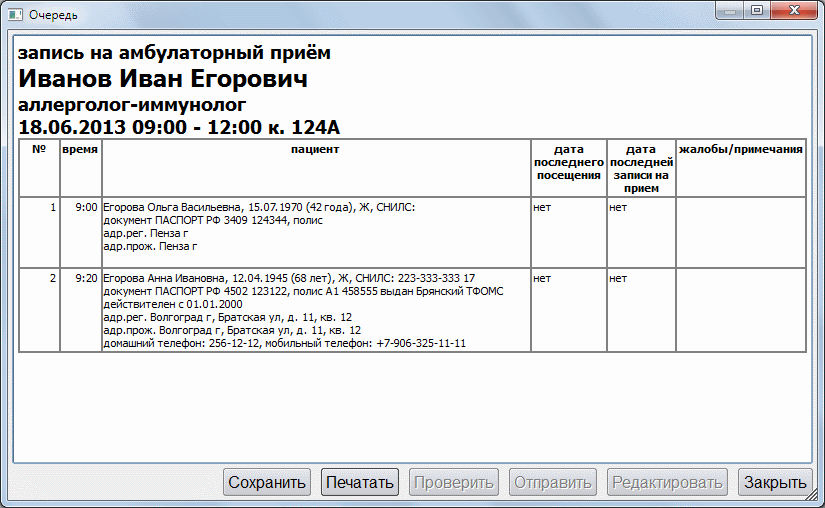
\includegraphics[width = 0.8\textwidth ,keepaspectratio]{pol_zaplist}
 \caption{Окно предварительного просмотра списка пациентов, записанных на прием}
 \label{img_pol_zaplist}
\end{figure}

В каждом из перечисленных случаев появится окно предварительного просмотра печати документа, содержащего список пациентов, записанных к выбранному врачу на выбранную дату. В зависимости от выбранного варианта печати, списки будут отличаться форматом заголовков и столбцов, составом столбцов и т.п. В каждом ЛПУ внешний вид списка так же может отличаться. Списки подтвержденных и неподтвержденных записей будут доступны, если в настройках выбрано использовать подтверждение записей. Тогда в список подтвержденных записей войдут те, которые отмечены знаком \putx~слева от фамилии пациента в списке предварительной записи, а в список неподтвержденных соответственно те, которые такой отметки не имеют. Пример списка пациентов приведен на рисунке \ref{img_pol_zaplist}.

Для печати списка нужно нажать кнопку \btn{Печатать}, для сохранения его в файл требуется нажать кнопку \btn{Сохранить} .

\subsection{Дополнительные возможности при работе со списком предварительной записи} \label{pol_zapdop}

Помимо всех описанных выше возможностей из списка предварительной записи пациентов (секция 5, Рисунок \ref{img_pol_zapgr}) можно выполнить следующее (для применения этих возможностей необходимо, чтобы в секции 5 отображался график врача на выбранную дату, а вызов контекстного меню осуществлялся на занятой строке):
\begin{itemize}
 \item \dm{Перейти в картотеку}. Выбор этого пункта из контекстного меню позволяет выбрать в картотеке пациента, который записан на текущий интервал времени и установить курсор на его карточке.
 \item \dm{Новое обращение}. Выбор этого пункта контекстного меню позволяет зарегистрировать обращение на основании записи на прием. Регистрация обращений подробно рассмотрена в разделе \ref{pol_obr}
 \item \dm{Свойства записи}. При выборе данного пункта меню открывается окно, содержащее информацию о пользователе, который зарегистрировал предварительную запись на прием, а так же более подробную информацию о записанном пациенте.
\end{itemize} 

\subsection{Вызов врача на дом} \label{pol_home}

Принцип регистрации вызовов врача на дом в \tmis~аналогичен предварительной записи на прием. Регистрация вызовов врача на дом так же осуществляется на панели \dm{Графики} (Рисунок \ref{img_pol_home}, секции 1 – 5). Если указанная панель отсутствует, ее нужно подключить в главном меню \mm{Настройки \str График}. После подключения в меню перед пунктом \dm{График} должен появиться установленный флажок \putx , а в левой части экрана соответствующая панель. Размеры отдельных секций панели можно регулировать с помощью мышки.

\begin{figure}[ht]\centering
 \includegraphics[width = 1\textwidth ,keepaspectratio]{pol_home}
 \caption{Регистрация вызова врача на дом}
 \label{img_pol_home}
\end{figure}

Для регистрации вызова врача на дом необходимо выполнить следующие действия:
\begin{enumerate}
 \item С помощью фильтра или любым другим способом нужно найти пациента в картотеке и установить курсор в секции 7 на его имени так, чтобы в секции 6 отображалась краткая информация о выбранном пациенте. Если пациент не был зарегистрирован ранее, его следует зарегистрировать в картотеке пациентов.
 \item В секции 1 необходимо выбрать подразделение ЛПУ, выполняющее вызовы на дом, раскрывая соответствующие ветви дерева, нажатием значка <<$+$>> слева от названия подразделения.
 \item В секции 2 следует найти специальность врача и, раскрыв список нажатием кнопки <<$+$>> слева от названия специальности, установить курсор на фамилии специалиста, к которому нужно записать пациента.
 \item В секции 3 на вкладке \dm{Календарь} необходимо выбрать дату приема, щелкнув по ней левой кнопкой мыши. По умолчанию выбрана текущая дата.
 \item В секции 4 нужно выбрать вкладку \dm{На дому}.
 \item В секции 5 будет отображен список интервалов времени для регистрации вызова врача на дом. В случае наличия свободного интервала следует щелкнуть по нему правой кнопкой мыши и в появившемся контекстном меню выбрать \dm{Поставить в очередь} или дважды щелкнуть левой кнопкой мыши по этому интервалу.
 \item В открывшемся окне (Рисунок \ref{img_pol_zhalobi}) выбрать из справочника слева или ввести с клавиатуры основные жалобы пациента и нажать кнопку \btn{OK}.
 \item Если пациент записан на прием успешно, то в поле \dm{ФИО} выбранного интервала появятся данные пациента. В секции 8 для этого пациента на вкладке \dm{Предварительная запись} так же добавится новая строка о предварительной записи к выбранному врачу.
\end{enumerate}

\begin{figure}[ht]\centering
 \includegraphics[width = 0.6\textwidth ,keepaspectratio]{pol_zhalobi}
 \caption{Окно редактирования жалоб пациента}
 \label{img_pol_zhalobi}
\end{figure}

Для удаления вызова врача на дом следует щелкнуть правой кнопкой мыши на соответствующей записи в секции 5 и в появившемся меню выбрать пункт \dm{Удалить из очереди}. То же действие можно выполнить, вызвав контекстное меню в секции 8.

Для редактирования жалоб пациента необходимо щелкнуть правой кнопкой мыши на соответствующей записи в секции 5 и в появившемся контекстном меню выбрать пункт \dm{Изменить жалобы\slash примечания}. Откроется окно \dm{Жалобы} (Рисунок \ref{img_pol_zhalobi}), куда следует внести изменения и сохранить их, нажав кнопку \btn{OK}.

В списке вызовов врача на дом (секция 5) существует возможность установки отметки о подтверждении записи. Для этого нужно установить флажок \putx~слева от фамилии пациента. Рекомендуется устанавливать отметку о подтверждении записи после передачи вызова врачу.

\begin{prim}
 Отметки о подтверждении записей могут отсутствовать, так как их наличие определяется настройками системы. Для подключения возможности установки отметок следует обратиться к администратору системы.
\end{prim}

Печать списка вызовов врача на дом аналогична печати списков предварительной записи на прием (см. раздел \ref{pol_zaplist}) 

О дополнительных возможностях при регистрации вызова врача на дом см. раздел \ref{pol_zapdop}

\subsection {Регистрация обращений} \label{pol_obr}

Каждый раз при обращении пациента в ЛПУ за амбулаторной или поликлинической помощью, в картотеке пациентов для него регистрируется новое обращение. Обращение содержит цель, установленные диагнозы пациента, результаты осмотров и обследований, информацию о назначенных мероприятиях и их выполнении, результат обращения. На основании обращения можно распечатать <<Талон амбулаторного пациента>> (Ф. 025\slash У).

Существует 3 способа регистрации поликлинического обращения в \tmis . Во всех случаях регистрация обращений производится из картотеки пациентов. Для перехода в картотеку пациентов нужно в главном меню выбрать пункт \mm{Работа \str Обслуживание пациентов}.

Способы регистрации обращений:
\begin{enumerate}
 \item Регистрация обращения на основе предварительной записи пациента из панели \dm{Графики}. Использование этого способа возможно, если в ЛПУ ведется предварительная запись на прием, и данный пациент был записан к соответствующему врачу. Так же необходимо, чтобы была подключена панель \dm{График}. Если она отсутствует, необходимо в главном меню выбрать пункт \mm{Настройки \str График}. Для регистрации обращения требуется на панели \dm{График} открыть список пациентов, записанных к указанному врачу на требуемую дату, найти нужного пациента в списке, щелкнуть на его фамилии правой кнопкой мыши и в контекстном меню выбрать пункт \dm{Новое обращение}.
 \item Регистрация обращения на основе предварительной записи пациента из картотеки пациентов. Использование этого способа возможно, если в ЛПУ ведется предварительная запись и пациент был записан к соответствующему врачу. Необходимо найти пациента в картотеке, используя фильтр или каким-либо иным способом, и щелкнуть по нему левой кнопкой мыши. При этом в верхней части окна картотеки появится общая информация о выбранном пациенте. В нижней части окна, на вкладке \dm{Предварительная запись} нужно найти запись пациента на прием к соответствующему специалисту, щелкнуть по ней правой кнопкой мыши и в контекстном меню выбрать пункт \dm{Новое обращение}.
 \item Регистрация обращения из вкладки \dm{Обращение}. Необходимо найти пациента в картотеке, используя фильтр или каким-то иным способом, и щелкнуть по нему левой кнопкой мыши. После этого следует перейти на вкладку \dm{Обращение} и нажить кнопку \btn{Новый (F9)} в нижней части окна или клавишу \keys{F9} на клавиатуре. Если кнопки не видны, можно перейти в нижнюю часть окна, используя полосу прокрутки справа.
\end{enumerate}
 
В результате выполнения любого из приведенных вариантов откроется окно \dm{Новое обращение} (Рисунок \ref{img_pol_obrnew}). В зависимости от выбранного способа и настроек системы, часть полей в разделе \dm{Основная информация} может быть заполнена.

\begin{figure}[ht]\centering
 \includegraphics[width = 1\textwidth ,keepaspectratio]{pol_obrnew}
 \caption{Регистрация нового обращения}
 \label{img_pol_obrnew}
\end{figure}

Прежде всего, необходимо проверить, что обращение создано для нужного пациента, сверив его данные в правой верхней части окна. После этого нужно заполнить пустые и изменить неверно заполненные поля в разделе \dm{Основная информация}.

\begin{vnim}
 Поле Дата выполнения на данном этапе заполнять не нужно!
\end{vnim}

Все поля, кроме поля \dm{Дата выполнения} являются обязательными для заполнения.
\begin{itemize}
 \item \dm{Организация} – наименование ЛПУ, в котором регистрируется случай обращения. По умолчанию указывается текущее ЛПУ.
 \item \dm{Тип обращения} выбирается из списка значение <<Поликлиника>>.
 \item \dm{Лечащий врач} – врач, к которому направляется пациент в поликлинике, в дальнейшем можно будет изменить лечащего врача.
 \item \dm{Источник финансирования} – канал оплаты обращения, выбирается из списка.
 \item \dm{Договор} – номер договора об оплате выбирается из списка. Состав списка зависит от выбранного источника финансирования.
 \item \dm{Тип события} – выбирается из списка. Состав списка изменяется в зависимости от выбранного типа обращения и источника финансирования.
 \item \dm{Отделение} – подразделение ЛПУ, куда направляется пациент.
 \item \dm{Дата начала} – по умолчанию устанавливается текущая дата и время. При необходимости дату и время можно изменить.
 \item \dm{Дата выполнения} – дата и время завершения обслуживания по данному обращению. Должна заполняться врачом.
\end{itemize}

После того как все поля заполнены верно, нужно нажать кнопку \btn{Создать}. Будет осуществлен переход к следующему этапу оформления обращения. Как правило, работа регистратуры ограничивается первым этапом. Последующее заполнение обращения выполняется врачом.

Если была предпринята попытка создания обращения не для того пациента или создание обращения вообще не требуется, следует нажать кнопку \btn{Отменить}. Обращение создано не будет.

\subsection {Вкладка «Обращение»}

Вкладка \dm{Обращение} предоставляет следующие возможности:
\begin{itemize}
 \item просмотр обращений выбранного пациента;
 \item просмотр состава обращения (диагнозы, мероприятия, посещения) без открытия карточки обращения;
 \item фильтрация обращений пациента;
 \item формирование списка обращений различных пациентов с помощью фильтров;
 \item печать списка обращений.
\end{itemize}

Так же из этой вкладки удобно создавать и редактировать обращения.

\begin{figure}[ht]\centering
 \includegraphics[width = 1\textwidth ,keepaspectratio]{pol_obrvkl}
 \caption{Внешний вид вкладки <<Обращение>>}
 \label{img_pol_obrvkl}
\end{figure}

Вкладка Обращение состоит из следующих секций (Рисунок \ref{img_pol_obrvkl}):
\begin{itemize}
 \item В верхней части окна (секция 1) содержится краткая информация о пациенте, выбранном на вкладке \dm{Пациенты}. По умолчанию показывается список обращений выбранного пациента.
 \item Секция 2 содержит список обращений выбранного пациента, либо список обращений, сформированный с помощью фильтра (секция 5).
 \item В секции 3 отображается подробная информация об обращении, на котором установлен курсор в секции 2. На вкладке \dm{Диагнозы} отображаются предварительные и заключительные диагнозы пациента; на вкладке \dm{Мероприятия} – все зарегистрированные медицинские документы пациента, направления на лабораторные и диагностические исследования, лечение; на вкладке \dm{Посещения} – список посещений пациента в составе выбранного обращения; на вкладке \dm{Примечание} – техническая информация о создании и обработке обращения.
 \item В секции 4 расположены кнопки для управления обращениями.
 \item В секции 5 расположены поля условий фильтра.
 \item В секции 6 – кнопки управления работой фильтра.
\end{itemize}

\subsection {Карточка обращения}

Карточка обращения состоит из нескольких разделов. Переключение между разделами осуществляется выбором соответствующего пункта на панели слева щелчком левой кнопки мыши:
\begin{itemize}
 \item Раздел \dm{Основная информация} содержит общие сведения о случае обслуживания, которые учитываются в стат.талоне и других документах;
 \item Раздел \dm{Медицинские документы} содержит направления на консультации и результаты осмотров врача;
 \item Раздел \dm{Диагностические и лабораторные исследования} содержит направления на исследования и их результаты;
 \item Раздел \dm{Лечение} содержит направление на медикаментозное, физиотерапевтическое и другие виды лечения и данные о их выполнении;
 \item Раздел \dm{Медико-экономические стандарты} дает возможность проверки соответствия назначений врача медико-экономическим стандартам по данному заболеванию.
 \item Раздел \dm{ВУТ} – позволяет зарегистрировать данные о временной нетрудоспособности пациента. 
 \item Раздел \dm{Оплата} – содержит данные, касающиеся оплаты для платных услуг.
\end{itemize}
 
Далее каждый из разделов будет рассмотрен более подробно.

\subsubsection{Основная информация}

В этом разделе часть данных заполняется на этапе создания случая обращения и в дальнейшем редактированию не подлежит (Рисунок \ref{img_pol_obroi}). Поля \dm{Лечащий врач}, \dm{Договор}, \dm{Дата начала}, первоначально введенные при создании случая обслуживания можно изменять. Данные об изменении лечащего врача сохраняются в таблице ниже. В колонке \dm{Врач} указывается ФИО врача, а в колонке \dm{Срок ответственности} – дата и время передачи пациента этому врачу.

\begin{figure}[ht]\centering
 \includegraphics[width = 1\textwidth ,keepaspectratio]{pol_obroi}
 \caption{Карточка редактирование обращения. Раздел <<Основная информация>>}
 \label{img_pol_obroi}
\end{figure}

В начале работы с обращением необходимо указать его \dm{Порядок} и \dm{Первичность}. При закрытии обращения нужно в поле \dm{Дата выполнения} ввести дату и время закрытия случая обслуживания, выбрать из списка значения \dm{Результат обращения} и \dm{Исход заболевания}.

В нижней части окна находится список посещений. При создании обращения автоматически создается первое посещение в соответствии с введенными данными при создании обращения. Можно добавить дополнительные посещения в список. Для этого необходимо дважды щелкнуть мышкой на пустой ячейке в колонке \dm{Место} и выбрать из списка значение, затем аналогичным образом заполнить ячейки \dm{Тип}, \dm{Услуга} и \dm{Тип финансирования}. В поле \dm{Дата} нужно внести дату нового посещения, используя клавиатуру или выбрав ее в календаре с помощью мыши.

\subsubsection{Медицинские документы} \label{pol_obr_md}

В данном разделе можно просмотреть, добавить или отредактировать результаты консультаций (осмотров) врачей по выбранному случаю обращения (Рисунок \ref{img_pol_obrmd}) и другие медицинские документы пациента.

\begin{figure}[ht]\centering
 \includegraphics[width = 1\textwidth ,keepaspectratio]{pol_obrmd}
 \caption{Карточка редактирование обращения. Раздел <<Медицинские документы>>}
 \label{img_pol_obrmd}
\end{figure}

Все медицинские документы по данному случаю обслуживания находятся в таблице в нижней половине окна. Над таблицей находится флажок \dm{Фильтр} и кнопка \btn{Создать}.

\paragraph{Фильтрация документов} \label{pol_obr_mdfiltr}

Фильтр позволяет найти нужные записи, если их слишком много в составе обращения. Для использования фильтра необходимо установить флажок \putx~\dm{Фильтр}, после чего появятся дополнительные поля для задания условий фильтрации (Рисунок \ref{img_pol_obrfiltr}):

\begin{figure}[ht]\centering
 \includegraphics[width = 1\textwidth ,keepaspectratio]{pol_obrfiltr}
 \caption{Карточка обращения. Фильтрация документов}
 \label{img_pol_obrfiltr}
\end{figure}

\begin{itemize}
 \item \dm{Выбор типа} – выбор типа документа для поиска из списка.
 \item \dm{Выбор категории} – выбор категории документа из списка. Состав списка зависит от значения, установленного в поле \dm{Выбор типа}. Если в этом поле выбрано значение <<Все типы>>, то данное поле недоступно для редактирования.
 \item \dm{Исполнитель} – выбор из списка исполнителя документа. Для консультаций исполнителем является врач, осуществляющий консультацию.
 \item \dm{Дата начала} и \dm{Дата окончания} задают период дат, за который осуществляется поиск документов.
 \item \dm{В работе} – при установке данного флажка в результаты фильтрации включаются незавершенные документы(находящиеся в процессе выполнения).
 \item \dm{Завершенные} – при установке данного флажка в результаты фильтрации включаются завершенные документы.
\end{itemize}
 
Использование одновременно флажков \dm{В работе} и \dm{Завершенные} обеспечивает поиск всех документов. Остальные параметры фильтрации связаны между собой по <<И>>, т.е. в результаты фильтрации попадают только те документы, для которых выполняются все условия одновременно.

После того как параметры фильтра заданы, необходимо нажать кнопку \btn{Применить} в правом нижнем углу области фильтра. Область фильтра будет скрыта, а на экране останутся лишь записи, удовлетворяющие условиям фильтрации. Если необходимо снова получить полный список, следует опять установить флажок \dm{Фильтр}, очистить все поля фильтра и нажать кнопку \btn{Применить} повторно.

\paragraph{Добавление нового документа} \label{pol_obr_mdnew}

При нажатии кнопки \btn{Создать}  откроется новое окно, содержащее список категорий документа. Список может быть представлен в двух видах: в виде простого списка или в виде дерева. Представление в виде списка расположено на вкладке \dm{Список} (Рисунок \ref{img_pol_obr_addd}). Для получения представления в виде дерева необходимо перейти на вкладку \dm{Дерево} (Рисунок \ref{img_pol_obr_addd2}). Раскрыть очередную ветку дерева можно, щелкнув левой кнопкой мыши по знаку <<$+$>> слева от названия типа документа. Для выбора категории документа в обоих случаях нужно дважды щелкнуть по выбранной строке левой кнопкой мыши.

Система запоминает представление, выбранное пользователем при предыдущем использовании, и при новом обращении открывает список категорий документов именно в таком виде. Поменять представление списка можно в любой момент, перейдя на другую вкладку.

\begin{figure}[ht]\centering
 \includegraphics[width = 1\textwidth ,keepaspectratio]{pol_obr_addd}
 \caption{Представление категорий документов в виде списка}
 \label{img_pol_obr_addd}
\end{figure}

\begin{figure}[ht]\centering
 \includegraphics[width = 1\textwidth ,keepaspectratio]{pol_obr_addd2}
 \caption{Представление категорий документов в виде дерева}
 \label{img_pol_obr_addd2}
\end{figure}

И в том, и в другом представлении можно воспользоваться поиском нужной категории. Для этого нужно в поле \dm{Поиск} ввести часть наименования категории. Список категорий будет фильтроваться по мере ввода текста в поле поиска. В результат поиска попадут категории, содержащие в названии образец поиска. Для возврата к полному списку категорий следует очистить поле поиска.

Флажок \dm{Только разрешенные в моем отделении} ограничивает список категорий лишь теми, которые разрешены в отделении к которому прикреплен пользователь. При необходимости можно снять данный флажок тогда список будет содержать все категории документов, доступные для создания данным пользователем.

\begin{prim}
 Для облегчения поиска список доступных категорий документов для конкретного пользователя (или группы пользователей) может быть ограничен настройками системы. Если в списке отсутствует документ, необходимый для работы, следует обратиться к администратору системы.
\end{prim} 

Для того чтобы создать документ, необходимо переместить соответствующую категорию в правую часть окна, в таблицу \dm{Выбранные действия}. Это можно сделать, дважды щелкнув по наименованию категории в левой части окна левой кнопкой мыши, либо перетащив ее из левой части окна в таблицу \dm{Выбранные действия} с помощью мыши. Обе операции выбора можно использовать как в представлении \dm{Список}, так и в представлении \dm{Дерево}. Можно выбрать сразу несколько категорий документов для создания, добавив их в список \dm{Выбранные действия}.
 
В качестве плановой даты выполнения по умолчанию для выбранных действий устанавливается текущая дата. Ее можно изменить вручную.

\begin{prim}
 Если сразу для нескольких документов необходимо изменить дату на одно и то же значение, то для оптимизации трудозатрат можно использовать следующий способ: 1) установить напротив соответствующих документов в разделе \dm{Выбранные действия} флажок \putx ; 2) нажать кнопку \btn{Установить дату} в правом нижнем углу окна  и 3) выбрать требуемую дату из календаря.
\end{prim} 
 
Для удаления ошибочно добавленных документов из списка \dm{Выбранные действия}, нужно щелкнуть правой кнопкой мыши по соответствующей строке и в появившемся контекстном меню выбрать пункт \dm{Удалить}.

\begin{prim}
 Для удаления одной или нескольких записей можно так же использовать следующий способ: установить напротив соответствующих документов в разделе \dm{Выбранные действия} флажок \putx~и нажать кнопку \btn{Удалить} в низу окна.
\end{prim} 
 
При нажатии кнопки \btn{OK}  откроется новое окно для заполнения созданного документа (Рисунок \ref{img_pol_obr_mdedt}). Если одновременно создавалось несколько документов, то после его закрытия, откроется следующее окно для заполнения второго документа из списка и т.д. пока не будут созданы все документы списка. Кнопка \btn{Отмена} в окне \dm{Создание действий} закрывает окно без сохранения (при повторной попытке создания документов потребуется заново формировать список выбора).

\paragraph{Редактирование медицинского документа} \label{pol_obr_mdedt}

\begin{figure}[ht]\centering
 \includegraphics[width = 1\textwidth ,keepaspectratio]{pol_obr_mdedt}
 \caption{Окно редактирования медицинского документа}
 \label{img_pol_obr_mdedt}
\end{figure}

В верхней части окна редактирования документа размещается общая информация о нем: состояние, дата и время начала и завершения формирования документа, исполнитель, количество процедур (для консультаций и осмотров это число всегда равно 1), УЕТ (заполняется только для стоматологических услуг), примечание. Как правило, если предыдущие шаги по созданию и редактированию случая обслуживания и медицинских документов в частности были верными, то все перечисленные выше поля заполнены верными значениями. Если это не так, то значения полей можно изменить.

В центральной части окна расположена основная часть документа, содержащая медицинскую информацию (Рисунок \ref{img_pol_obr_mdedt}). В левой половине ее расположена таблица, содержащая данные медицинского документа. Порядок заполнения полей таблицы следующий: необходимо дважды щелкнуть левой кнопкой мыши по пустой ячейке в столбце \dm{Значение}, тем самым активировав возможность редактирования данного поля, затем выбрать из списка или ввести с клавиатуры данные, соответствующие названию строки, расположенному в первой колонке таблицы.

В зависимости от настроек, становится доступным один из следующих типов заполнения полей:
\begin{enumerate}
 \item Предоставляет наиболее широкие возможности. При активации поля, оно расширяется и становится доступным текстовый редактор, позволяющий вводить произвольный текст и форматировать его. В правой части окна появляется тезаурус, содержащий набор наиболее часто встречающихся формулировок для выбранного поля. Тезаурус представляет собой дерево, для раскрытия ветвей которого следует нажать кнопку <<$+$>> слева от требуемой ветки. Двойной щелчок по какой-либо фразе или слову в тезаурусе добавит ее(его) в поле текстового редактора на место, где находился курсор в момент добавления. Фразы, добавленные из тезауруса, также подлежат редактированию и форматированию в текстовом редакторе (Рисунок \ref{img_pol_obr_mdedt1}). В тезаурусе при этом они не изменяются.
 
 \begin{figure}[ht!]\centering
  \includegraphics[width = 1\textwidth ,keepaspectratio]{pol_obr_mdedt1}
  \caption{Заполнение документа с помощью тезауруса}
  \label{img_pol_obr_mdedt1}
 \end{figure}
 
 \item Представляет собой только текстовый редактор с возможностью ввода произвольного текста и его последующего форматирования, но не содержит тезаурус. Такие поля используются в случаях, когда невозможно выделить какие-либо общие фразы для указанного поля (Рисунок \ref{img_pol_obr_mdedt2}).
 
  \begin{figure}[ht!]\centering
   \includegraphics[width = 1\textwidth ,keepaspectratio]{pol_obr_mdedt2}
   \caption{Заполнение документа с помощью текстового редактора}
   \label{img_pol_obr_mdedt2}
  \end{figure}
 
 \item Представляет собой поле со списком, из которого требуется выбрать единственное значение (Рисунок \ref{img_pol_obr_mdedt3}).
 \item Представляет собой поле, в которое можно с клавиатуры ввести какое-либо значение (число, дату, строку).
\end{enumerate}

 \begin{figure}[ht!]\centering
   \includegraphics[width = 1\textwidth ,keepaspectratio]{pol_obr_mdedt3}
   \caption{Выбор значения из списка}
   \label{img_pol_obr_mdedt3}
 \end{figure}
  
Заполнив описанными выше методами все поля медицинского документа, следует сохранить его. Для этого нужно нажать кнопку \btn{Сохранить}, в результате чего окно редактирования текущего документа закроется, а данные о новом документе появятся в разделе \dm{Медицинские документы} обращения. Кнопка \btn{Закрыть} закрывает окно редактирования документа без сохранения.

Для вывода на печать полученного документа нужно нажать кнопку \btn{Печать} в правом нижнем углу окна, и, при необходимости, выбрать из появившегося меню вид печатной формы. Откроется окно предварительного просмотра печатной формы (Рисунок \ref{img_pol_obr_mdprn}), где следует нажать кнопку \btn{Печатать} для отправки документа на принтер.

 \begin{figure}[ht]\centering
   \includegraphics[width = 0.7\textwidth ,keepaspectratio]{pol_obr_mdprn}
   \caption{Предварительный просмотр печати медицинского документа}
   \label{img_pol_obr_mdprn}
 \end{figure}
 
Если что-либо в полученной печатной форме не устраивает, можно нажать кнопку \btn{Редактор}  в нижней части окна редактирования медицинского документа, и, при необходимости, выбрать из появившегося меню вид печатной формы. Откроется окно, содержащее ту же самую печатную форму, но здесь она доступна для редактирования и форматирования (Рисунок \ref{img_pol_obr_mdedt4}). Внесенные в документ изменения можно сохранить, нажав кнопку \btn{Сохранить} в окне редактора документа.

\begin{vnim}
 Сохраненные в окне редактора документа  изменения будут отображаться только в этом окне. Сохраненные изменения будут отображаться в окне редактора при повторном входе.
\end{vnim}
 
Для печати отредактированного документа необходимо нажать кнопку \btn{Печать} непосредственно из окна редактора.

 \begin{figure}[ht]\centering
   \includegraphics[width = 0.9\textwidth ,keepaspectratio]{pol_obr_mdedt4}
   \caption{Окно редактирования медицинского документа}
   \label{img_pol_obr_mdedt4}
 \end{figure}

Кнопки \btn{Сохранить шаблон}  и \btn{Загрузить шаблон}  дают возможность многократного использования результатов заполнения документа. Подробнее работа с шаблонами будет рассмотрена в разделе \ref{pol_pattern}

\begin{prim}
 Зачастую пациенты обращаются по поводу одного и того же заболевания многократно. Результаты осмотра (консультации) врача при этом получаются во многом идентичными. Для облегчения работы врача в таких случаях в \tmis~предусмотрена кнопка \btn{Копировать из предыдущего}. При ее нажатии автоматически находится последний документ такого же типа среди предыдущих обращений пациента, и результаты его заполнения копируются в текущий документ. При этом можно отредактировать текущий документ, а предыдущий останется в прежнем виде.
\end{prim}

В левом нижнем углу окна редактирования медицинского документа имеются кнопки  \btn{$\gg$}, \btn{$\ll$}, \btn{>\rule{1pt}{8pt}}  и \btn{\rule{1pt}{8pt}<}. Эти кнопки предназначены для перемещения по медицинским документам текущего обращения. При нажатии на кнопки  \btn{>\rule{1pt}{8pt}}  и \btn{\rule{1pt}{8pt}<}   в текущем окне отображается соответственно первый и последний документ в составе обращения, кнопки  \btn{$\gg$} и \btn{$\ll$} отвечают за отображение предыдущего и следующего медицинского документа в составе обращения.

\paragraph{Дополнительные возможности при работе с действиями}

\tmis~предоставляет ряд дополнительных возможностей по работе с медицинскими документами. Для доступа к ним необходимо щелкнуть правой кнопкой мыши по документу в списке (Рисунок \ref{img_pol_obrmd}) и в появившемся контекстном меню выбрать один из следующих пунктов:
\begin{itemize}
 \item \dm{Открыть действие только для чтения}. При выборе данного пункта открывается карточка выбранного документа, только для просмотра. Редактирование открытого таким образом документа будет невозможно, что позволяет избежать риска случайного изменения данных при просмотре. Открытие документа только на чтение, к тому же, позволяет просматривать его нескольким пользователям одновременно.  
 \item При выборе пункта \dm{Дублировать действие} создается и открывается на редактирование медицинский документ того же типа, что и выбранный. При этом в верхней части карточки указываются текущие даты и исполнитель, а основная часть оказывается заполненной, как в исходном документе. Во вновьсозданный документ можно внести дополнительные изменения и сохранить его. При этом исходный документ не изменится, а новый документ будет добавлен в обращение.   
 \item В отличии от предыдущего пункта, пункт \dm{Создать такое же} позволяет создать и открыть на редактирование новый документ того же типа, что и исходный, но основная его чать будет незаполнена.
 \item \dm{Удалить действие} -- удаление документа из обращения. Для выполнения данного действия требуется подтвердить его в дополнительном диалоговом окне, нажав кнопку \btn{Продолжить} 
 \item Пункт \dm{Печать} позволяет открыть окно предварительного просмотра печати выбранного медицинского документа, не открывая его карточку.
\end{itemize}

  
\subsubsection{Раздел «Диагностические и лабораторные исследования»} \label{pol_obr_is}

В данном разделе (Рисунок \ref{img_pol_obris}) существует возможность:
\begin{itemize}
 \item регистрации направлений на диагностические и лабораторные исследования;
 \item просмотра зарегистрированных направлений и результатов выполненных исследований;
 \item ввода результатов лабораторных и диагностических исследований.
\end{itemize}

 \begin{figure}[ht]\centering
   \includegraphics[width = 1\textwidth ,keepaspectratio]{pol_obris}
   \caption{Карточка обращения. Раздел <<Диагностические и лабораторные исследования>>}
   \label{img_pol_obris}
 \end{figure}
 
Последнее из описанных действий, в данном разделе представляет собой дополнительную возможность, т.к. для ввода результатов существует другое, более удобное, окно.

Как и в предыдущем разделе, присутствует возможность фильтрации записей. Работа фильтра аналогична описанной в разделе \ref{pol_obr_mdfiltr} В качестве исполнителя здесь следует выбирать врача-лаборанта или врача-диагноста соответственно, выполнившего (или назначенного на выполнение) исследования. При задании периода дат в параметрах фильтрации, фильтр будет установлен по дате направления, а не выполнения исследования.

При нажатии кнопки \btn{Создать}  откроется новое окно, содержащее список доступных для назначения исследований. Список может быть представлен в двух видах: в виде простого списка или в виде дерева. Представление в виде списка расположено на вкладке \dm{Список} (Рисунок \ref{img_pol_obr_isedt}). Для получения представления в виде дерева необходимо перейти на вкладку \dm{Дерево}. Раскрыть очередную ветку дерева можно, щелкнув левой кнопкой мыши по знаку <<$+$>> слева от названия типа документа. Для выбора категории документа в обоих случаях нужно дважды щелкнуть по выбранной строке левой кнопкой мыши.

Система запоминает представление, выбранное пользователем при предыдущем использовании, и при новом обращении открывает список исследований именно в таком виде. Поменять представление списка исследований можно в любой момент, перейдя на другую вкладку.

 \begin{figure}[ht]\centering
   \includegraphics[width = 1\textwidth ,keepaspectratio]{pol_obr_isedt}
   \caption{Список исследований в виде списка}
   \label{img_pol_obr_isedt}
 \end{figure}  
 
И в том, и в другом представлении можно воспользоваться поиском нужного исследования. Для этого нужно в поле \dm{Поиск} ввести часть его наименования. Исследования  будут фильтроваться по мере ввода текста в поле поиска. В результат поиска попадут исследования, содержащие в названии образец поиска. Для возврата к полному списку исследований следует очистить поле поиска.

Флажок \dm{Только разрешенные в моем отделении} ограничивает список исследований лишь теми, которые разрешено назначать в отделении, к которому прикреплен пользователь. При необходимости можно снять данный флажок, тогда список будет содержать все исследования, доступные для использования данным пользователем.

\begin{prim}
 Для облегчения поиска список доступных исследований для конкретного пользователя (или группы пользователей) может быть ограничен настройками системы. Если в списке отсутствует исследование, необходимое для работы, следует обратиться к администратору системы.
\end{prim}
  
После того, как нужное исследование найдено, для выбора его к назначению следует дважды щелкнуть по строке с наименованием исследования левой кнопкой мыши либо перетащить его из левой части окна в правую с помощью мыши. При этом исследование будет добавлено в список \dm{Выбранные действия} в правой половине окна. Можно добавить сразу несколько исследований к назначению, а затем нажать кнопку \btn{OK} в правом нижнем углу окна (Рисунок \ref{img_pol_obr_isedt}). Все выбранные исследования будут добавлены в список в разделе \dm{Диагностические и лабораторные исследования} (Рисунок \ref{img_pol_obris}).

По умолчанию в качестве плановой даты выполнения для выбранных исследований устанавливается 7:00 следующего дня. Ее можно изменить вручную после добавления направления к назначению, либо после назначения исследования, открыв карточку направления на редактирование.

\begin{prim}
 Если сразу для нескольких исследований нужно изменить дату на одно и то же значение, то для оптимизации трудозатрат можно использовать следующий способ: 1) установить напротив соответствующих документов в разделе \dm{Выбранные действия} флажок \putx ; 2) нажать кнопку \btn{Установить дату} в правом нижнем углу окна и 3) выбрать требуемую дату из календаря.
\end{prim}

Для удаления ошибочно добавленных документов из списка \dm{Выбранные действия}, нужно щелкнуть правой кнопкой мыши по соответствующей строке и в появившемся контекстном меню выбрать пункт \dm{Удалить}.

\begin{prim}
 Для удаления одной или нескольких записей можно так же использовать следующий способ: установить напротив соответствующих документов в разделе \dm{Выбранные действия} флажок \putx~и нажать кнопку \btn{Удалить} в низу окна.
\end{prim}

Открыть направление для редактирования можно несколькими способами:
\begin{itemize}
 \item дважды щелкнуть по нему левой кнопкой мыши;
 \item выделить его в списке направлений щелчком левой кнопки мыши и нажать клавишу \keys{F4};
 \item щелкнуть правой кнопкой мыши по выбранному направлению и в появившемся меню выбрать \dm{Открыть действие}.
\end{itemize}

В результате любого из описанных действий откроется карточка исследования (Рисунок \ref{img_pol_obr_iscard}). Внешний вид карточки исследования может различаться в зависимости от типа исследования.

 \begin{figure}[ht]\centering
   \includegraphics[width = 1\textwidth ,keepaspectratio]{pol_obr_iscard}
   \caption{Карточка редактирования направления на лабораторное исследование}
   \label{img_pol_obr_iscard}
 \end{figure} 
 
Поля, выделенные рамкой на рисунке \ref{img_pol_obr_iscard}, должны заполняться при создании направления. Остальные поля заполняются при вводе результата исследования.
\begin{itemize}
 \item \dm{Назначено} – содержит дату и время создания направления;
 \item Флажок \dm{Срочно} устанавливается для срочных исследований;
 \item \dm{План} – планируемые дата и время выполнения исследования, если оно не является срочным;
 \item \dm{Назначил} – фамилия назначившего врача, по умолчанию указывается фамилия пользователя, зарегистрировавшего направление;
 \item \dm{Тип биоматериала} должен быть выбран из списка, если для исследования может использоваться различный биоматериал;
 \item В колонке \dm{Назначено} таблицы требуется оставить флажки только напротив тех параметров, которые необходимо исследовать. Эта возможность присутствует только для лабораторных исследований.
\end{itemize}
 
Для сохранения введенных данных необходимо нажать кнопку \btn{Сохранить}.

\paragraph{Ввод результатов функциональной диагностики} \label{pol_obr_isrez}

Ввод результатов исследований состоит из 2-х этапов: заполнение шапки и заполнение медицинской информации в таблице (Рисунок \ref{img_pol_obr_isrez}).

Шапка документа состоит из следующих полей:
\begin{itemize}
 \item \dm{Состояние} – выбирается из списка. После того, как  исследование выполнено, необходимо перевести его в статус <<Завершено>>;
 \item \dm{Начато} – дата начала выполнения, заполняется автоматически в момент создания назначения и устанавливается равной текущей дате;
 \item \dm{Выполнено} – дата завершения выполнения. При изменении значения в поле \dm{Состояние} на <<Закончено>>, в данном поле автоматически устанавливается текущая дата;
 \item \dm{Штрих-код} исследования, заполняется для лабораторных исследований при интеграции с ЛИС;
 \item \dm{Исполнитель} – фамилия специалиста, выполнившего исследование, выбирается из списка;
 \item \dm{Кабинет} – номер кабинета, в котором было выполнено исследование;
 \item \dm{УЕТ} – как правило, заполняется только для стоматологии;
 \item \dm{Примечание} – дополнительная информация.
\end{itemize}

 \begin{figure}[ht]\centering
   \includegraphics[width = 1\textwidth ,keepaspectratio]{pol_obr_isrez}
   \caption{Карточка редактирования результатов функциональной диагностики}
   \label{img_pol_obr_isrez}
 \end{figure}
 
Принцип заполнения табличной части аналогичен описанному в разделе \ref{pol_obr_mdedt} Единственное отличие состоит в том, что в таблицу добавлен дополнительный столбец \dm{Ед.изм.}, содержащий единицу измерения для числовых величин. Cтолбец \dm{Ед.изм.} не подлежит редактированию.

% При наличии на диагностическом оборудовании возможности создавать архив результатов исследований в формате DICOM, можно организовать связь с результатами пациента. Тогда врач сможет воспользоваться этой связью и просмотреть результат пациента. Для создания связи необходимо нажать кнопку \btn{DICOM Архив} в правой нижней части окна и из открывшегося меню выбрать пункт \dm{Сопоставить с DICOM Архивом}. Откроется диалоговое окно, где необходимо указать имя или номер файла и нажать кнопку \btn{Сохранить}.

% Для просмотра связанного DICOM-файла результата, нужно нажать кнопку \btn{DICOM Архив} в правой нижней части окна и из открывшегося меню выбрать пункт \btn{Просмотр на DICOM Архиве}. После этого откроется окно просмотра результата исследования в формате DICOM.

% Если связь с DICOM-файлом была создана ошибочно, можно разорвать ее, нажав кнопку \btn{DICOM Архив} в правой нижней части окна и выбрав пункт \dm{Отменить сопоставление с DICOM Архивом}. После разрыва связи, можно создать связь с правильным файлом.

Для вывода на печать заключения врача по результатам исследования необходимо нажать кнопку \btn{Печать} в правом нижнем углу окна. Откроется окно предварительного просмотра печати (Рисунок \ref{img_pol_obr_isprn}). Для отправки документа на принтер необходимо нажать кнопку \btn{Печатать}.

 \begin{figure}[ht]\centering
   \includegraphics[width = 0.8\textwidth ,keepaspectratio]{pol_obr_isprn}
   \caption{Окно предварительного просмотра заключения}
   \label{img_pol_obr_isprn}
 \end{figure}

\paragraph{Ввод результатов лабораторных исследований} \label{pol_obr_rez}
 
%Методика работы врача-лаборанта по занесению результатов лабораторных исследований будет рассмотрена в разделе ... 
В данном разделе будет рассмотрена методика работы врача по вводу единичных результатов лабораторных исследований.

Заполнение шапки результата лабораторного исследования аналогично описанному в пп. \ref{pol_obr_isrez}

Табличная часть результата лабораторного исследования состоит из 5-ти столбцов (Рисунок \ref{img_pol_obr_isrez2}):

 \begin{figure}[ht]\centering
   \includegraphics[width = 1\textwidth ,keepaspectratio]{pol_obr_isrez2}
   \caption{Карточка результатов лабораторного исследования}
   \label{img_pol_obr_isrez2}
 \end{figure}
 
\begin{itemize}
 \item \dm{Название параметра} -- наименование параметра исследования;
 \item \dm{Назначено} –- отметка о необходимости исследования данного параметра, устанавливается врачом при назначении. При выполнении состояние этого столбца изменять не следует;
 \item \dm{Значение} –- результат исследования для текущего параметра;
 \item \dm{Ед.изм.} -– единица измерения параметра, не подлежит редактированию, служит для правильного ввода и интерпретации результата;
 \item \dm{Норма} –- границы нормы для параметра, не подлежит редактированию, служит для правильной интерпретации результата.
\end{itemize}

 \begin{figure}[h!]\centering
   \includegraphics[width = 0.6\textwidth ,keepaspectratio]{pol_obr_isprn2}
   \caption{Окно предварительного просмотра печати результата лабораторного исследования}
   \label{img_pol_obr_isprn2}
 \end{figure}

При вводе результатов следует заполнять только столбец \dm{Значение}. Для повышения скорости ввода результатов рекомендуется использовать клавиши \keys{↑} и \keys{↓} на клавиатуре для перехода по строкам и клавишу \keys{Enter} для подтверждения ввода результата.
 
После заполнения результатов исследования, его можно вывести на печать. Для этого следует нажать кнопку \btn{Печать} в правом нижнем углу окна. Откроется окно предварительного просмотра печати (Рисунок \ref{img_pol_obr_isprn2}). Для отправки документа на принтер необходимо нажать кнопку \btn{Печатать}.  

\subsubsection{Раздел «Лечение»} \label{pol_obr_lek}

Данный раздел предназначен для регистрации направлений на медикаментозное, физиотерапевтическое, оперативное и другие виды лечения, а так же для контроля их выполнения.

Логика работы данного раздела практически полностью повторяет логику работы предыдущих двух разделов, поэтому приводить повторное описание работы не целесообразно.

Работа с фильтрами аналогична приведенной в разделе \ref{pol_obr_mdfiltr} Регистрация нового назначения аналогична описанной в разделе \ref{pol_obr_mdnew} При регистрации нового назначения карточка лечения открывается для редактирования. Необходимо заполнить поля \dm{Дата назначения}, \dm{Срочно}, \dm{План}, \dm{Назначил}, а так же заполнить табличную часть (Рисунок \ref{img_pol_obr_lek}). Заполнение шапки таблицы аналогично приведенному в разделе \ref{pol_obr_isrez} Заполнение табличной части подробно описано в разделе \ref{pol_obr_rez}

 \begin{figure}[ht]\centering
   \includegraphics[width = 1\textwidth ,keepaspectratio]{pol_obr_lek}
   \caption{Карточка назначения лечения}
   \label{img_pol_obr_lek}
 \end{figure}
 
После того как все данные внесены, необходимо сохранить назначение, нажав кнопку \btn{Сохранить}  в правом нижнем углу окна.

Для печати назначения следует нажать кнопку \btn{Печать}. Откроется окно предварительного просмотра печати. Для отправки документа на принтер нужно нажать кнопку \btn{Печатать}.

\subsubsection{Раздел «Медико-экономические стандарты»}

В данном разделе можно выбрать МЭС для обращения и проверить соответствие назначений врача выбранному МЭС.

\subsubsection{ВУТ} \label{pol_vut}

В данном разделе можно зарегистрировать сведения о временной нетрудоспособности, возникшие в рамках случая обращения.

В разделе (Рисунок \ref{img_pol_obr_vut}) имеется 4 вкладки:
\begin{itemize}
 \item \dm{ВУТ} -- для учета листков временной нетрудоспособности пациента;
 \item \dm{Справка} -- для учета временной нетрудоспособности неработающих пациентов, для которых не требуется оформление листка временной нетрудоспособности;
 \item \dm{Инвалидность} -- для учета инвалидностей пациента, возникших в рамках случая обращения;
 \item \dm{Ограничения жизнедеятельности} -- для учета справок по ограничению физической и других видов нагрузки пациента.
\end{itemize}

 \begin{figure}[ht]\centering
   \includegraphics[width = 1\textwidth ,keepaspectratio]{pol_obr_vut}
   \caption{Карточка обращения. Раздел <<ВУТ>>}
   \label{img_pol_obr_vut}
 \end{figure}
 
Вкладки заполняются в соответствии с документми о временной нетрудоспособности, выданными пациенту. Если в рамках данного случая обращения пациенту не было выдано документов о временной нетрудоспособности, то данный раздел не заполняется.

Чтобы внести данные на одну из вкладок, необходимо установить сответствующий флажок в левом верхнем углу вкладки, после чего станут доступными для заполнения следующие поля:
\begin{itemize}
 \item \dm{Причина} -- причина выдачи документа о временной нетрудоспособности, выбирается из списка. Поле является обязательным для заполнения.
 \item \dm{Доп. причина} -- дополнительная причина, может выбираться из справочника для некоторых видов причин нетрудоспособности. 
 \item \dm{Серия} -- серия документа о  нетрудоспособности, выданного пациенту. Вводится с клавиатуры. Обязательна для заполнения только для документов строгого учета.
 \item \dm{Номер} -- номер документа о нетрудоспособности, выданного пациенту. Заполняется с клавиатуры. Поле обязательно для заполнения.
 \item \dm{Занятость} -- тип занятости, выбирается из списка.
 \item \dm{Место работы} -- место работы пациента (место предоставления документа о нетрудоспособности), вводится с клавиатуры.
\end{itemize}

Следующие поля недоступны для редактирования. Они заполняются автоматически на основе данных, внесенных в другие поля:
\begin{itemize}
 \item \dm{Длительность} -- длительность нетрудоспособности (в днях) по данному документу. Расчитывается на основе всех записей, внесенных в таблицу ниже.
 \item \dm{Вне ЛПУ} -- количество дней нетрудоспособности, не связанных с госпитализацией.
 \item \dm{Пол} -- пол пациента, берется из карточки пациента.
 \item \dm{Возраст} -- возраст пациента, берется из карточки пациента.
 \item \dm{Продлен} -- серия и номер документа о временной нетрудоспособности, продолжением которого является данный документ.
 \item \dm{Дата начала ВУТ} -- заполняется только при оформлении продолжения ВУТ. В даннном поле указывается дата начала первого листа нетрудоспособности по данному случаю.
 \item \dm{Дней} -- общее число дней нетрудоспособности по данному случаю. 
\end{itemize}

После заполнения полей в верхней части вкладки, следует заполнить поля табличной части. В зависимости от выбранной вкладки и типа нетрудоспособности, табличная часть может содержать одну или несколько записей. Например, при оформлении листка временной нетрудоспособности, в табличнуу часть должна добавляться запись каждый раз при продлении листка временной нетрудоспособности.

Таблица содержит следующие поля:
\begin{itemize}
 \item \dm{Начало} -- дата начала нетрудоспособности (для первой записи) или периода нетрудоспособности (для последующих записей).
 \item \dm{Окончание} -- дата окончания нетрудоспособности (для последней записи) или периода нетрудоспособности (для остальных записей).
 \item \dm{Длительность} -- длительность периода нетрудоспособности. Рассчитывается автоматически на основе даты начала и окончания париода нетрудоспособности.
 \item \dm{Результат} -- результат периода нетрудоспособности, выбирается из списка.
 \item \dm{Закончивший} -- врач, закрывший период нетрудоспособности, выбирается из списка.
 \item \dm{Режим} -- рекомендуемый режим, выбирается из списка.
 \item \dm{Нарушение} -- заполняется только в случае, если документ о нетрудоспособности закрыт по причине нарушения режима. Значение выбирается из списка.
 \item \dm{Примечание} -- в данное поле может быть внесена любая дополнительная информация.
 \item \dm{Внешний} -- флажок должен быть установлен, если период зарегистрирован в другом ЛПУ.
 \item \dm{Начавший} -- врач, зарегистрировавший период нетрудоспособности, выбирается из списка.
 \item \dm{Направлен на КЭК} -- дата направления на КЭК. Заполняется, в случае направление пациента на КЭК в рамках данного случая обращения.
 \item \dm{Дата КЭК} -- дата проведения КЭК. Заполняется, в случае направление пациента на КЭК в рамках данного случая обращения.
 \item \dm{Эксперт} -- врач, проводивший КЭК, выбирается из списка. Заполняется, в случае направление пациента на КЭК в рамках данного случая обращения.
 \item \dm{Номер путевки} -- номер путевки на КЭК. Заполняется, в случае направление пациента на КЭК в рамках данного случая обращения.
 \item \dm{Дата1} -- дата начала инвалидности. Заполняется, в случае присвоения пациенту инвалидности в рамках данного обращения.
 \item \dm{Дата2} -- дата окончания срока инвалидности по результатам КЭК. Заполняется, в случае присвоения пациенту инвалидности в рамках данного обращения.
 \item \dm{Группа инвалидности} -- группа инвалидности по результатам КЭК, выбирается из списка. Заполняется, в случае присвоения пациенту инвалидности в рамках данного обращения.
\end{itemize} 

Для добавления записи в таблицу следует внести данные в ее пустую строку. Для удаления записи из таблицы следует щелкнуть правой кнопкой мыши по этой страке и в появившемся контекстном меню выбрать пункт \dm{Удалить текущую строку}.

Для оформления продолжения листка временной нетрудоспособности необходимо нажать кнопку \btn{Продлить}, расположенную справа от поля \dm{Место работы}, и заполнить поля \dm{Серия} и \dm{Номер}, указав в них данные нового документа временной нетрудоспособности. Данные предыдущего документа появятся в полях \dm{Продлен}, \dm{Дата начала ВУТ}, \dm{Дней}.

После добавления или редактирования данных о временной нетрудоспособности следует сохранить внесенные данные нажатием кнопки \btn{Сохранить} в правом нижнем углу окна.
   
\subsubsection{Раздел «Оплата»}

В данном разделе содержатся сведения о согласовании услуг, заключенном договоре и оплате при совершении платных медицинских услуг.

На вкладке \dm{Согласование} находится информация о заключенном договоре на оказание платных медицинских услуг. На вкладке \dm{Услуги} – перечень услуг, оказанных пациенту. На вкладке \dm{Расчет} – информация о платежах пациента.
Более подробно данный раздел будет рассмотрен в главе <<Платные медицинские услуги>>.

\subsubsection{Сохранение предварительных диагнозов пациента} \label{pol_diag2}

Для добавления предварительного диагноза в текущем обращении следует перейти в раздел \dm{Основная информация} и нажать кнопку \btn{Предварительные диагнозы} в центральной части окна. В открывшемся окне (Рисунок \ref{img_pol_diag1}) необходимо заполнить данные о предварительных диагнозах пациента, последовательно заполняя каждую ячейку строки. Большинство значений в ячейках выбирается из списка. Активировать список можно, дважды щелкнув по ячейке левой кнопкой мыши.

 \begin{figure}[ht]\centering
   \includegraphics[width = 1\textwidth ,keepaspectratio]{pol_diag1}
   \caption{Предварительные диагнозы пациента}
   \label{img_pol_diag1}
 \end{figure}
 
Рассмотрим состав полей для описания предварительного диагноза более подробно:
\begin{itemize}
 \item \dm{Тип диагноза} (основной или сопутствующий) выбирается из справочника. Для каждого обращения может быть задан только один основной и несколько сопутствующих диагнозов. Поле обязательно для заполнения.
 \item \dm{Врач} – фамилия врача, установившего диагноз. По умолчанию устанавливается фамилия врача, указанного в обращении в качестве лечащего.
 \item \dm{МКБ} – код диагноза по МКБ-10. Возможен поиск диагноза в справочнике или выбор его из дерева. Поле обязательно для заполнения.
 \item \dm{Доп.МКБ} – расширение кода МКБ.
 \item \dm{Хар.} – характер заболевания выбирается из справочника.
 \item \dm{Фаза} выбирается из справочника для онкологических заболеваний.
 \item \dm{Ст} – стадия заболевания, выбирается из справочника.
 \item \dm{ДН} – отношение к диспансерному учету, выбирается из справочника.
 \item \dm{Травма} – тип травмы выбирается из справочника. Поле заполняется при наличии травмы у пациента.
 \item \dm{ГрЗд} – группа здоровья пациента, выбирается из справочника.
 \item \dm{Описание} – уточненная формулировка диагноза.
\end{itemize}
  
После того как все предварительные диагнозы внесены, необходимо нажать кнопку \btn{Сохранить}. Внесенные данные будут сохранены, а окно редактирования предварительных диагнозов закроется.

Для удаления диагноза из списка следует щелкнуть правой кнопкой мыши на этом диагнозе и в появившемся меню выбрать пункт \dm{Удалить диагноз}.

\subsubsection{Сохранение заключительных диагнозов пациента}

Для добавления заключительного диагноза в текущем обращении следует в разделе \dm{Основная информация} нажать кнопку \btn{Окончательные диагнозы} в центральной части окна. Добавление заключительного диагноза производится аналогично добавлению предварительного диагноза (см. раздел \ref{pol_diag2}) Возможно добавление только одного заключительного основного диагноза и нескольких осложнений и сопутствующих заболеваний.

После того, как все заключительные диагнозы внесены, необходимо нажать кнопку \btn{Сохранить}. Заключительные диагнозы будут сохранены, а окно их редактирования закроется.

\subsubsection{Закрытие случая обращения}

После того как лечение пациента по данному случаю обращения завершено, обращение необходимо закрыть. Закрытие обращения говорит о том, что активная работа с данным пациентом по данному случаю обращения завершена. После закрытия редактирование обращения становится невозможным. Как правило, статистический учет и выставление счетов СМО производится только по закрытым обращениям.

\begin{vnim}
 Закрытие обращения выполняется без дополнительных подтверждений и является необратимой операцией! Будьте внимательны при закрытии обращений!
\end{vnim} 
 
Перед закрытием обращения необходимо указать заключительный диагноз пациента, а так же заполнить поля \dm{Результат обращения} и \dm{Исход заболевания} в разделе \dm{Основная информация}. Заполнение поля \dm{Результат обращения} является обязательным условием для закрытия обращения. Обязательность заполнения поля \dm{Исход заболевания} определяется настройками системы.

Для закрытия обращения необходимо нажать кнопку \btn{Закрыть обращение} в левом нижнем углу окна. Если данные о результате лечения не были заполнены, появится соответствующее предупреждение. Если все необходимые поля заполнены, будет произведено закрытие случая обращения и появится сообщение об успешном выполнении операции.

\begin{vnim}
 Кнопка \btn{Удалить} в левом нижнем углу окна обращения удаляет случай обращения полностью!
\end{vnim} 

\subsection{Редактирование обращения}

Для редактирования обращения следует выбрать в главном меню пункт \mm{Работа \str Обслуживание пациентов}. В открывшемся окне необходимо найти соответствующее обращение на вкладке \dm{Обращения} и нажать кнопку \btn{Редактировать (F4)} в нижней части окна (если кнопки не видны, рекомендуется воспользоваться полосой прокрутки справа) или клавишу \keys{F4} на клавиатуре. В результате любого из этих действий откроется окно редактирования обращения. Структура карточки обращения и способы ее редактирования подробно рассмотрены выше (см. раздел \ref{pol_obr})

После того, как все изменения внесены в карточку обращения, нужно нажать кнопку \btn{Сохранить} для сохранения сделанных изменений, а затем кнопку \btn{Выйти без сохранения} для закрытия карточки обращения.

\subsection{Создание и использование индивидуальных шаблонов медицинских документов} \label{pol_pattern}

Очень часто встречаются ситуации, когда врач в течении своего рабочего дня вынужден заполнять десятки однотипных осмотров, которые отличаются друг от друга всего лишь несколькими словами или фразами. Либо у врача существует 2-5 основных заболеваний, результат осмотра по каждому из которых, практически идентичен. В этих случаях врачу рекомендуется воспользоваться механизмом сохранения и последующей загрузки шаблонов медицинских документов. Шаблон можно создать для любого из медицинских документов разделов \dm{Движение пациента}, \dm{Медицинские документы}, \dm{Диагностические и лабораторные исследования}, \dm{Лечение}, однако наиболее часто они используются для заполнения результатов осмотров врачей и результатов диагностических исследований.

 \begin{figure}[ht!]\centering
   \includegraphics[width = 1\textwidth ,keepaspectratio]{pol_pattern1}
   \caption{Медицинский документ для сохранения в качестве шаблона}
   \label{img_pol_pattern1}
 \end{figure}
 
Принцип работы с шаблонами следующий. Врач заполняет табличную часть типового медицинского документа (Рисунок \ref{img_pol_pattern1}) и сохраняет его в качестве шаблона (Рисунок \ref{img_pol_pattern2}). Каждый врач может сохранить любое количество различных шаблонов для одного или нескольких медицинских документов только для себя или для всех пользователей.
 
 \begin{figure}[ht!]\centering
   \includegraphics[width = 0.6\textwidth ,keepaspectratio]{pol_pattern2}
   \caption{Сохранение нового шаблона}
   \label{img_pol_pattern2}
 \end{figure}
 
В дальнейшем, при загрузке шаблона, табличная часть нового медицинского документа будет заполнена так же, как табличная часть документа, ранее сохраненного в качестве шаблона. В текущем документе после загрузки шаблона можно поменять значения некоторых полей (подчеркнуто синим на рисунке \ref{img_pol_pattern3}) и сохранить документ. При этом внесенные изменения сохранятся в документе, а шаблон останется неизменным (Рисунок \ref{img_pol_pattern3}).

 \begin{figure}[h!]\centering
   \includegraphics[width = 1\textwidth ,keepaspectratio]{pol_pattern3}
   \caption{Результат использования шаблона при заполнении документа}
   \label{img_pol_pattern3}
 \end{figure}
 
\subsubsection{Создание нового шаблона документа} 

Для создания нового шаблона документа следует заполнить новый документ или открыть какой-либо из ранее сохраненных документов, подходящих для использования в качестве шаблона, и нажать кнопку \btn{Сохранить шаблон} в левом нижнем углу окна редактирования документа. Откроется окно сохранения шаблона (Рисунок \ref{img_pol_pattern2}).

Для создания нового шаблона необходимо в левой части окна выбрать группу в дереве шаблонов, куда следует добавить новый шаблон, щелкнув левой кнопкой мыши по корневому элементу выбранной группы (для добавления шаблона в корень дерева следует установить курсор на корневом элементе дерева соответственно), и нажать кнопку \btn{Создать шаблон}. Во вновь открывшемся окне (Рисунок \ref{img_pol_pattern4}) нужно задать свойства сохраняемого шаблона и нажать кнопку \btn{OK}. 

 \begin{figure}[h!]\centering
   \includegraphics[width = 0.5\textwidth ,keepaspectratio]{pol_pattern4}
   \caption{Окно создания шаблона}
   \label{img_pol_pattern4}
 \end{figure}
 
Созданный шаблон будет доступен только для медицинских документов того вида, к которому относится исходный документ для создания шаблона. Т.е. если в примере, приведенном выше, шаблон создавался на основе документа <<Врач-гастроэнтеролог (Консультация врача-специалиста или врача-специалиста высшей категории, или кандидата медицинских наук)>>, то он будет доступен для загрузки только для медицинских документов, имеющих такое же наименование. Так же можно указать ограничения на использование шаблона при его создании:
\begin{itemize}
 \item \dm{Пол} – если поле заполнено, то шаблон будет доступен только при заполнении медицинских документов пациентов выбранного пола.
 \item \dm{Возраст} – если введены возрастные границы в поля ввода, то шаблон будет доступен только при заполнении медицинских документов пациентов указанной возрастной группы. При указании возрастных границ необходимо так же выбирать единицу измерения возраста из списка слева от соответствующего поля ввода (Д – дни, Н – недели, М – месяцы, Г – годы).
 \item Группа переключателей \dm{Этот шаблон могут применять} позволяет определить, для кого из пользователей будет виден данный шаблон. При установке переключателя на значение <<Врач>>, необходимо из списка выбрать фамилию врача, тогда шаблон будет доступен только для выбранного пользователя. При установке переключателя на значение <<Специальность>>, необходимо из списка справа выбрать название специальности, тогда шаблон будет доступен только тем пользователям, у которых в настройках системы указана выбранная специальность. Установка переключателя на значение <<Все>> делает шаблон доступным для всех пользователей.
\end{itemize}

Для сохранения созданного шаблона необходимо нажать кнопку \btn{OK}. При нажатии кнопки \btn{Отмена} окно создания шаблона будет закрыто без сохранения внесенных в него данных.

При нажатии на кнопку \btn{Сохранить шаблон} в окне \dm{Сохранение шаблона действия} (Рисунок \ref{img_pol_pattern2}) ранее сохраненный шаблон заменяется шаблоном текущего документа.

Для создания новой группы в дереве шаблонов (Рисунок \ref{img_pol_pattern2}) следует установить курсор на корень дерева (для добавления группы в корень) или на корневой элемент той группы, в которой следует создать подгруппу, и нажать кнопку \btn{Создать группу}. В появившемся окне нужно ввести название новой группы и нажать кнопку \btn{OK}. Группа будет добавлена в указанное место.

\subsubsection{Загрузка шаблона документа}

Для загрузки ранее созданного шаблона следует создать или открыть незаполненный документ соответствующего вида и нажать кнопку \btn{Загрузить шаблон}. В раскрывшемся дереве доступных шаблонов нужно выбрать подходящий, дважды щелкнув по нему левой кнопкой мыши. В результате, значения всех полей табличной части документа изменятся на значения из шаблона. Если значение какого-либо поля в шаблоне отсутствует, то в текущем документе при загрузке шаблона оно не изменится. После того, как шаблон был загружен, значения полей текущего документа можно редактировать. При этом значения полей в самом шаблоне останутся неизменным. Для сохранения внесенных в документ изменений следует нажать кнопку \btn{Сохранить}.

\subsection{Фильтрация обращений} \label{pol_obr_filtr}

Фильтр обращений расположен в правой части окна на вкладке \dm{Обращение} (Рисунок \ref{img_pol_obrvkl}, секция 5). Возможно применение фильтра к обращениям одного пациента, группы пациентов или всем обращениям, зарегистрированным в системе.

В верхней части панели \dm{Фильтр} находятся следующие поля фильтрации обращений: \dm{Назначение}, \dm{Тип обращения}, \dm{Источник финансирования}, \dm{Тип}. Их значения выбираются из справочников. Далее, панель фильтров разбивается на 2 вкладки: \dm{Поиск} и \dm{Расширенный}. На вкладке \dm{Поиск} содержатся наиболее часто используемые параметры поиска и фильтрации обращений, на вкладке \dm{Расширенный} содержатся специальные параметры фильтрации, которые могут использоваться для выявления ошибок и в обращениях и других дополнительных функций.

Можно совместно использовать параметры фильтрации из обеих вкладок и верхней части панели. Все условия фильтрации при этом будут связаны по <<И>>, т.е. в результат отбора попадут только те обращения, для которых будут выполняться все условия одновременно.

Для того чтобы включить в условия фильтрации какой-либо параметр, следует установить напротив него флажок \putx , а затем выбрать из списка или ввести значение параметра.

Вкладка \dm{Поиск} содержит следующие параметры отбора:
\begin{itemize}
 \item \dm{Дата назначения}. В результаты поиска попадают обращения, дата назначения которых попадает в период дат, указанный в фильтре.
 \item \dm{Не выполнено}. Результат будет включать обращения, у которых не заполнено поле \dm{Дата выполнения}.
 \item \dm{Дата выполнения}. Результат будет включать обращения, у которых дата выполнения попадает в заданный период дат.
 \item \dm{Специальность} – специальность лечащего врача.
 \item \dm{Врач} – фамилия лечащего врача. Данное поле является связанным с полем \dm{Специальность}. Если поле \dm{Специальность} заполнено, то в текущем поле отобразится список врачей только выбранной специальности.
 \item Флажок \dm{Состоит на ДН} позволяет отобрать пациентов, состоящих на диспансерном учете.
 \item Поле \dm{ЛПУ} позволяет выбрать обращения, зарегистрированные в выбранном ЛПУ (если несколько ЛПУ используют одну базу данных).
 \item Флажок \dm{Любое, кроме базового} позволяет выбрать случаи обращения, зарегистрированные на другие ЛПУ (кроме ЛПУ пользователя).
 \item \dm{Код МЭС} позволяет найти обращения с указанным кодом МЭС.
 \item \dm{Результат} – результат обращения.
\end{itemize}
 
Вкладка \dm{Расширенный} содержит следующие поля отбора:
\begin{itemize}
 \item \dm{Автор} – фильтрация по имени пользователя, создавшего (зарегистрировавшего) обращение.
 \item \dm{Дата создания}. В результаты фильтрации попадают обращения, дата создания которых попадает в период дат, указанный в фильтре. В большинстве случаев дата создания и дата назначения совпадают, т.к. по умолчанию в поле \dm{Дата назначения} записывается текущая дата, но дату назначения можно изменить при создании обращения, поэтому фильтрация по данному полю не является дублированием поиска по дате назначения.
 \item \dm{Автор последнего изменения} – фильтрация по имени пользователя, внесшего последние изменения в карточку обращения.
 \item \dm{Дата последнего изменения}. В результат фильтрации попадают обращения, дата последнего изменения которых попадает в указанный период дат.
 \item Флажок \dm{Ошибки в закл. диагнозе} позволяет отобрать случаи обращения, содержащие ошибки в заключительном диагнозе.
 \item \dm{Оплата}. В первом поле следует выбрать состояние оплаты, а во втором – источник финансирования обращений. В результате фильтрации будут получены обращения, оплата которых находится в указанном состоянии по указанному источнику финансирования.
 \item \dm{Код карточки} – поиск по коду обращения.
 \item \dm{Внешний идентификатор} – поиск по внешнему идентификатору обращения.
 \item Флажок \dm{Только закрытые истории болезни} позволяет отобрать только случаи обращения, для которых выполнено закрытие.
\end{itemize}
 
После того как параметры фильтрации установлены, необходимо нажать кнопку \btn{Применить}. В результате в секции 2 (Рисунок \ref{img_pol_obrvkl}) отобразится список обращений, удовлетворяющих условиям фильтрации.

Для получения полного списка обращений (снятия фильтра) нужно нажать кнопку \btn{Сбросить} и снова кнопку \btn{Применить}.

Поле \dm{Показать осмотры} в нижней части панели фильтра (Рисунок \ref{img_pol_obrvkl}, секция 6) определяет область действия фильтра. При выборе значения данного поля <<пациента из картотеки>>, фильтр будет применен к обращениям пациента, указанного в секции 1 (Рисунок \ref{img_pol_obrvkl}). Выбор пункта <<пациентов из картотеки>> в указанном поле приведет к тому, что в результат фильтрации попадут обращения всех пациентов, которые в данный момент отображаются на вкладке \dm{Пациенты}. При выборе значения <<Все>> фильтр будет применяться к обращениям всех пациентов, зарегистрированных в текущей базе данных.

Рассмотрим использование опции \dm{Показывать осмотры} на примерах.

\textbf{\textit{Пример 1.}} Требуется показать незавершенные случаи обслуживания пациента Боброва П.Ф.

Для получения результата следует выполнить следующую последовательность действий:
\begin{enumerate}
 \item На вкладке \dm{Пациенты} установить фильтр \dm{Фамилия} = <<Бобров>>, \dm{Имя} = <<П>> и нажать кнопку \btn{Применить}.
 \item В полученном списке результатов найти пациента Боброва П.Ф. и щелкнуть по нему левой кнопкой мыши.
 \item Перейти на вкладку \dm{Обращение}.
 \item На панели \dm{Фильтр} вкладка \dm{Поиск} установить флажок \dm{Не выполнено}.
 \item В поле \dm{Показывать осмотры} выбрать значение <<пациента из картотеки>> и нажать кнопку \btn{Применить}.
\end{enumerate}
 
\textbf{\textit{Пример 2.}} Найти все случаи обращения в поликлинику пациентов из г. Санкт-Петербурга за последний месяц.

Для получения требуемого результата необходимо выполнить следующую последовательность действий:
\begin{enumerate}
 \item На вкладке \dm{Пациенты} установить фильтр \dm{Адрес} =<<«Регистрации>>, а в следующем поле выбрать из списка <<Санкт-Петербург г>> и дважды щелкнуть по нему левой кнопкой мыши, нажать кнопку \dm{Применить}.
 \item Перейти на вкладку \dm{Обращение} и на панели \dm{Фильтр} выбрать \dm{Тип обращения} = <<Поликлиника>>.
 \item В поле \dm{Показывать осмотры} выбрать значение <<пациентов из картотеки>> и нажать кнопку \btn{Применить}.
\end{enumerate}
 
\textbf {\textit {Пример 3.}} Получить список активных (не закрытых) обращений врача Иванова И.П.

Для получения указанного результата требуется:
\begin{enumerate}
 \item На панели \dm{Фильтр} вкладки \dm{Обращение} установить флажок \dm{Не выполнено}, в поле \dm{Врач} выбрать значение <<Иванов И.П.>>
 \item В поле \dm{Показывать осмотры} выбрать значение <<все>> и нажать кнопку \btn{Применить}.
\end{enumerate}

\subsection{Обслуживание пациентов} \label{pol_obsl}

В картотеке пациентов на вкладке \dm{Обслуживание} работа ведется не с обращениями, а с отдельными медицинскими записями пациента или пациентов.
На этой вкладке имеется возможность:
\begin{itemize}
 \item Просмотреть все медицинские записи выбранного пациента за всю историю его обращений, не заходя при этом в карточки обращений.
 \item Выбрать все записи определенного типа, состояния, исполнителя и т.п. за всю историю обращений пациента, минуя карточки обращений.
 \item Выбрать все медицинские записи по типу, исполнителю, состоянию, дате назначения для группы пациентов или всех пациентов картотеки.
\end{itemize}

Данная вкладка может быть очень удобна лечащему врачу для просмотра и анализа анамнеза заболеваний пациента, а так же врачам диагностических (и других) подразделений для поиска направленных к ним пациентов и заполнения результатов исследований (консультаций).

В верхней части окна на вкладке \dm{Обслуживание} отображается краткая информация о пациенте, которому принадлежит выбранный в данный момент медицинский документ (Рисунок \ref{img_pol_serv}). Ниже, в правой части окна находится панель фильтрации данных. В левой части окна располагается список, отобранных с помощью фильтра, медицинских документов пациента.

 \begin{figure}[ht]\centering
   \includegraphics[width = 1\textwidth ,keepaspectratio]{pol_serv}
   \caption{Вкладка <<Обслуживание>>}
   \label{img_pol_serv}
 \end{figure}
 
Список документов пациента разбит на 4 вкладки:
\begin{enumerate}
 \item Вкладка \dm{Статус} содержит записи об осмотрах, консультациях врачей, эпикризах и других документах, расположенных в разделе \dm{Медицинские документы} карточки обращения.
 \item Вкладка \dm{Диагностика} содержит информацию о лабораторных и диагностических исследованиях пациента.
 \item Вкладка \dm{Лечение} содержит записи о назначении физиотерапевтических, медикаментозных и других видах лечения.
 \item Вкладка \dm{Мероприятия} содержит информацию о движении пациента в стационаре и планировании госпитализаций.
\end{enumerate} 

Для просмотра содержимого документа, нужно выбрать его из списка, щелкнув по нему левой кнопкой мыши. Содержимое документа будет отображено в нижней части окна.

Для открытия карточки документа на редактирование можно дважды щелкнуть по нему левой кнопкой мыши либо нажать клавишу \keys{F4} на клавиатуре либо нажать кнопку \btn{Редактировать (F4)}  в нижней части окна. Для открытия карточки обращения, в состав которого входит документ, нужно нажать кнопку \btn{Редактировать обращение} в левом нижнем углу окна.

При нажатии на кнопку \btn{Печать (F6)} открывается окно предварительного просмотра списка документов, отображаемых в данный момент на экране.

Фильтр разбит на 2 вкладки: \dm{Поиск} и \dm{Расширенный поиск}. В верхней части расположено поле выбора типа документа, которое доступно с обеих вкладок фильтра. \dm{Тип} документа выбирается из справочника типов документов, представленного в виде дерева. Выбор значения из справочника осуществляется двойным щелчком левой кнопки мыши.

Вкладка \dm{Поиск} содержит наиболее часто использующиеся параметры отбора документов:
\begin{itemize}
 \item \dm{Дата назначения} – позволяет отобрать документы по дате назначения, указанной в них. Необходимо указать дату начала и дату окончания периода для отбора. Дата начала периода должна быть обязательно заполнена. Дата окончания периода может оставаться пустой, тогда поиск будет осуществляться за период от даты начала до текущего момента.
 \item \dm{Специальность назначившего} – выбирается из списка специальность назначившего врача.
 \item \dm{Назначил} – фамилия назначившего врача, выбирается из списка.
 \item При установке флажка \dm{Срочно} в результаты выборки попадут только мероприятия, назначенные по cito.
 \item \dm{Плановая дата выполнения} – позволяет отобрать назначения, запланированные на определенную дату или период дат. Необходимо указать дату начала и дату окончания периода для отбора.
 \item \dm{Состояние} выполнения назначения, выбирается из списка.
 \item \dm{Дата выполнения} – позволяет отобрать документы по дате выполнения. Необходимо указать дату начала и дату окончания периода для отбора.
 \item \dm{Специальность исполнителя} – выбирается из списка.
 \item \dm{Исполнитель} – фамилия исполнителя выбирается из списка.
\end{itemize}

 \begin{figure}[ht]\centering
   \includegraphics[width = 1\textwidth ,keepaspectratio]{pol_serv_dop}
   \caption{Вкладка <<Обслуживание>>. Расширенный поиск}
   \label{img_pol_serv_dop}
 \end{figure}
 
Вкладка \dm{Расширенный поиск} предоставляет дополнительные возможности поиска (Рисунок \ref{img_pol_serv_dop}). Чаще всего они используются администраторами системы и другим техническим персоналом. Расширенный поиск предоставляет возможности фильтрации по следующим параметрам:
\begin{itemize}
 \item \dm{Автор} – можно выполнить поиск документов, зарегистрированных указанным пользователем. Фамилия пользователя выбирается из списка. На предыдущей вкладке имеется похожее поле \dm{Назначил}.  Отличие их заключается в том, что значение поля \dm{Назначил} пользователь может изменить вручную, а значение текущего поля недоступно для редактирования. Например, если регистрацию назначений врача ведет медсестра, войдя под своим идентификатором, то в поле  \dm{Назначил} она укажет фамилию врача, а в поле \dm{Автор} сохранится фамилия медсестры.
 \item \dm{Дата создания} – позволяет отобрать документы по дате их создания. Необходимо указать дату начала и дату окончания периода для отбора. Дата начала должна быть обязательно заполнена. Дата окончания может оставаться пустой. В отличии от \dm{Даты назначения}, которая может изменяться пользователем, \dm{Дата создания} документа недоступна для редактирования. Например, если врач заполняет истории болезни за предыдущий день, то в качестве даты назначения он укажет предыдущий день, а в поле \dm{Дата создания} будет сохранена текущая дата.
 \item \dm{Автор последнего изменения} – можно выполнить поиск по фамилии пользователя, внесшего последние изменения в документ.
 \item \dm{Дата последнего изменения} – позволяет отобрать документы по системной дате их последнего изменения. Необходимо указать даты начала и окончания периода. Дата начала должна быть обязательно заполнена. Дата окончания может оставаться пустой.
 \item \dm{Оплата} – позволяет отобрать мероприятия, оплата которых находится в выбранном состоянии по указанному источнику финансирования. При выборе данного параметра фильтрации, требуется заполнить 2 поля, выбрав их значения из списка: состояние оплаты и источник финансирования мероприятия.
 \item \dm{Учитывать свойства} – использование данного параметра целесообразно только при выборе определенного значения в поле \dm{Тип} документа в верхней части фильтра. При установке флажка \dm{Список свойств}, в поле ниже появляется список свойств документа, выбранного типа. Необходимо установить флажки напротив названий тех свойств, состояние которых требуется определить. Если флажок \dm{Заполнено\slash Не заполнено} установлен, то будет осуществлен поиск документов, в которых указанные свойства заполнены. Если этот флажок снят, то будет выполнен поиск документов , где выбранные свойства не заполнены.
\end{itemize}
 
Для добавления параметра поиска следует напротив соответствующего поля фильтра установить флажок \putx , а затем, в ставшее активным поле, ввести искомое значение параметра. Параметры фильтра связаны между собой по <<И>>, т.е. в результаты поиска попадут записи, удовлетворяющие всем условиям поиска одновременно. Возможно одновременное использование параметров со вкладок \dm{Поиск} и \dm{Расширенный поиск}. Они так же будут связаны между собой по <<И>>.

В нижней части панели фильтрации находится поле выбора области поиска. Необходимо выбрать из списка одно из следующих значений:
\begin{itemize}
 \item Пациента из картотеки – поиск будет осуществлен среди документов пациента, выбранного на вкладке \dm{Пациенты}.
 \item Пациентов из картотеки – поиск будет осуществлен среди документов всех пациентов, отображаемых в данный момент на вкладке \dm{Пациенты}.
 \item Осмотра из вкладки обращение – поиск документов будет осуществлен в составе обращения, выбранного на вкладке \dm{Обращение}.
 \item Осмотров из вкладки обращение – поиск документов будет осуществлен среди документов всех обращений, отображаемых на вкладке \dm{Обращение} в текущий момент. В ряде случаев результаты поиска при выборе текущей области поиска и области поиска <<Пациента из картотеки>> могут совпадать. Но они будут отличаться, если на вкладке \dm{Обращение} предварительно была применена фильтрация обращений.
 \item Все – поиск документов будет осуществлен среди всех документов, зарегистрированных в \tmis.
\end{itemize}
 
После того, как все параметры поиска и область поиска заданы, необходимо нажать кнопку \btn{Применить} . В левой части окна отобразится список документов, полученный в результате поиска. Для возврата фильтра к настройкам по умолчанию нужно нажать кнопку \btn{Сбросить} , а затем снова \btn{Применить} , чтобы изменения вступили в силу.

\subsection{Регистрация медицинских осмотров}

Медицинский осмотр является частным случаем обращения пациента в поликлинику.

При регистрации обращения с типом события «Диспансеризация», «Медицинский осмотр» и т.п. требуется в поле \dm{Лечащий врач} указать фамилию врача (чаще всего терапевта), который будет оформлять заключение по медицинскому осмотру. 

После нажатия кнопки \btn{ОК} в окне создания документа откроется окно \dm{Планировщик} (Рисунок \ref{img_pol_plan}), где необходимо отметить флагом \putx~мероприятия, которые должны быть выполнены в составе медицинского осмотра.

 \begin{figure}[ht!]\centering
   \includegraphics[width = 0.8\textwidth ,keepaspectratio]{pol_plan}
   \caption{Окно планировщика}
   \label{img_pol_plan}
 \end{figure}
 
После нажатии кнопки \btn{OK} в окне планировщика будет создано обращение, в соответствующие разделы которого будут добавлены отмеченные ранее мероприятия. Мероприятия будут находиться в состоянии <<Начато>>. 

Использование данного механизма освобождает медицинский персонал от рутинного добавления в большом количестве медицинских документов и направлений на исследования. Врач должен будет найти соответствующий медицинский документ в составе обращения, заполнить его, перевести в состояние <<Закончено>> и сохранить сделанные изменения.

После получения данных всех осмотров врачей-специалистов, результатов лабораторных и диагностических исследований лечащий врач должен оформить заключение по диспансеризации, заполнить результат обращения и закрыть обращение.

\begin{prim}
Состав мероприятий, отображаемых в планировщике, определяется настройками системы. Для изменения состава мероприятий, следует обратиться к администратору системы
\end{prim} %3. Расписание
  \newpage
\section{Обслуживание пациентов}

\subsection {Регистрация обращений} \label{pol_obr}

Каждый раз при обращении пациента в ЛПУ за амбулаторной помощью, в картотеке пациентов для него регистрируется новое обращение. Обращение содержит цель, установленные диагнозы пациента, результаты осмотров и обследований, информацию о назначенных мероприятиях и их выполнении, результат обращения. На основании обращения можно распечатать <<Талон амбулаторного пациента>> (Ф. 025\slash У-12).

Для регистрации обращения на основе предварительной записи следует найти данные пациента в БД (см. п. \ref{cl_find}) и щелкнуть по соответствующей записи левой кнопкой мыши. В появившемся всплывающем окне (Рисунок \ref{img_cl_contrwin}) нужно нажать кнопку \includegraphics[scale=0.6]{addg}, справа от соответствующей записи на вкладке \dm{Предварительная запись}. Будет открыта страница \dm{Создание обращения}.

Кнопки \btn{Создать обращение} или \includegraphics[scale=0.6]{addb} позволяют создавать обращение без предварительной записи. Кнопки доступны:
\begin{itemize}
 \item Из высплывающего окна картотеки пациентов (Рисунок \ref{img_cl_contrwin});
 \item Со страницы создания и редактирования регистрационной карточки пациента. 
\end{itemize}

Дле регистрации обращения без предварительной записи нужно нажать кнопку \btn{Создать обращение} или кнопку \includegraphics[scale=0.6]{addb}. Если на момент регистрации обращения у пациента имеются действующие предварительные записи к другим специалистам, то появится предупреждение во всплывающем окне <<У пациента есть предварительные записи>>.Необходимо убедиться, что предварительные записи были зарегистрированы к другому врачу и только после этого продолжить регистрацию текущего обращения нажатием кнопки \btn{Все равно продолжить}. Отменить создание обращения без предварительной записи можно, нажав кнопку  \btn{Отмена} во всплывающем окне.

После подтверждения будет открыта страница \dm{Создание обращения}. На этой странице, прежде всего, необходимо убедиться, что обращение создано для нужного пациента, проверив его данные в правой верхней части окна. После этого нужно заполнить пустые и изменить неверно заполненные поля в блоке \dm{Основная информация}. Часть полей может быть заполнена на основе данных предварительной записи (если обращение создавалось на основе нее) или значениями по умолчанию.

\begin{vnim}
 Поля \dm{Дата выполнения} и \dm{Время выполнения} на данном этапе заполнять не нужно!
\end{vnim}

Все поля, кроме полей \dm{Дата выполнения} и \dm{Время выполнения} являются обязательными для заполнения.
\begin{itemize}
 \item \dm{Тип обращения} выбирается из списка значение <<Поликлиника>>.
 \item \dm{Источник финансирования} – канал оплаты обращения, выбирается из списка.
 \item \dm{Договор} – номер договора об оплате выбирается из списка. Состав списка зависит от выбранного источника финансирования.
 \item \dm{Тип события} – выбирается из списка. Состав списка изменяется в зависимости от выбранного типа обращения и источника финансирования.
 \item \dm{Лечащий врач} – врач, к которому направляется пациент в поликлинике.
 \item \dm{Подразделение} – отделение поликлиники, куда направляется пациент.
 \item \dm{Дата начала} – по умолчанию устанавливается дата предварительной записи либо текущая дата. При необходимости дату можно изменить.
 \item \dm{Время начала} – по умолчанию устанавливается время предварительной записи либо текущее время. При необходимости время можно изменить.
 \item \dm{Дата выполнения} – дата завершения обслуживания по данному обращению. Должна заполняться врачом.
 \item \dm{Время выполнения} – время закрытия обращения. Должно заполняться врачом.
\end{itemize}

После того как все поля заполнены верно, нужно нажать кнопку \btn{Создать} в правом нижнем углу страницы. Будет осуществлен переход к следующему этапу оформления обращения. Как правило, работа регистратуры ограничивается первым этапом. Последующее заполнение обращения выполняется врачом.

Если была предпринята попытка создания обращения не для того пациента или создание обращения вообще не требуется, следует нажать кнопку \btn{Отменить}. Обращение создано не будет.

\subsubsection{Регистрация платных обращений}

Если в качестве источника финансирования обращения выбрано <<Платные услуги>>, то необходимо на странице обращения зарегистрировать данные о плательщике (Рисунок \ref{img_pol_payer}). Рекомендуется сделать это при создании обращения. Однако, можно ввести эти данные и позднее, открыв обращение на редактирование. 

\begin{figure}[ht]\centering
	\includegraphics[width = 1\textwidth ,keepaspectratio]{pol_payer}
	\caption{Данные плательщика в обращении}
	\label{img_pol_payer}
\end{figure}

В качестве плательщика может выступать физическое или юридическое лицо.

Если плательщиком является физическое лицо, то необходимо заполнить следующие поля в подразделе \dm{Плательщик} на вкладке \dm{Физ.лицо}:
\begin{itemize}
	\item \dm{Фамилия} -- фамилия плательщика;
	\item \dm{Имя} -- имя плательщика;
	\item \dm{Отчество} -- отчество плательщика;
	\item \dm{Дата рождения} -- дата рождения плательщика;
	\item \dm{Документ} -- тип документа, удостоверяющего личность плательщика. Выбирается из раскрывающегося списка;
	\item \dm{Серия} -- серия документа, удостоверяющего личность плательщика. Серия может быть разбита на 2 отдельных поля;
	\item \dm{Номер} -- номер документа, удостоверяющего личность плательщика. 
	\item \dm{Серия} -- серия документа, удостоверяющего личность плательщика;
	\item \dm{Адрес} -- адрес регистрации плательщика, записывается в виде текстовой строки. 
\end{itemize}

Кнопки, расположенные справа от полей подраздела \dm{Плательщик}, позволяют в некоторых случаях автоматизировать заполнение данных полей. 
\begin{itemize}
	\item Кнопка \btn{карты пациента} позволяет скопировать в поля подраздела \dm{Плательщик} на вкладке \dm{Физ.лицо} данные пациента. Данную кнопку можно применять, если сам пациент является плательщиком.
	\item Кнопка \btn{карты родственника} позволяет скопировать в поля подраздела \dm{Плательщик} на вкладке \dm{Физ.лицо} данные одного из родственников пациента. При нажатии на данную кнопку появляется всплывающее окно, где необходимо выбрать одного из родственноков пациента и нажать кнопку \btn{Выбрать}. Для использования данного способа необходимо, чтобы родственник пациента был зарегистрирован в разделе \dm{Связи} регистрационной карточки текущего пациента.
	\item Кнопка \dm{предыдущего} позволяет скопировать данные плательщика из предыдущего обращения пациента (если такое имеется).
\end{itemize} 

Если плательщиком является юридическое лицо, то необходимо перейти на вкладку \dm{Юр.лицо} в подразделе \dm{Плательщик} и выбрать название организации-плательщика из раскрывающегося списка. Вверху списка предусмотрено поле поиска организации. Список организаций фильтруется в соответствии с текстом, введенным в поле поиска. Все необходимые реквизиты организации-плательщика должны быть заполнены в справочнике организаций и не требуют повторного заполнения.

\subsubsection{Регистрация услуг}

В случае обращения пациента за медицинскими услугами на платной основе, необходимо зарегистрировать список услуг, которые будут оказаны пациенту, согласовать стоимость и оформить договор на оказание соответствующих услуг.

Регистрация услуг выполняется на странице редактирования обращения (Рисунок \ref{img_pol_usl}). Необходимо ввести часть наименования услуги в поле поиска, после чего выбрать нужную запись или несколько записей, появившихся в списке ниже, щелкнув по ним левой кнопкой мыши. Выбранные строки появятся в списке \dm{Выбранные услуги}.

\begin{figure}[ht]\centering
	\includegraphics[width = 1\textwidth ,keepaspectratio]{pol_usl}
	\caption{Регистрация услуг в обращении}
	\label{img_pol_usl}
\end{figure}

Для выбранных услуг можно изменить количество в ячейке \dm{Количество} и установить флажок \dm{Считать} для включения стоимость услуг в итоговую сумму в строке <<Итого к оплате>> под таблицей. 

После регистрации требуемого набора услуг необходимо сохранить обращение, после чего распечатать договор и другие платежные документы, нажав кнопку \includegraphics[scale=0.6]{print}, выбрав соответствующие пункты из списка и нажав кнопку \btn{Печать}.



\subsection{Обслуживание пациентов (для врача)} \label{pol_ttbl_new}
Если в ЛПУ ведется предварительная запись пациентов на прием по расписанию, то обслуживание пациентов врачом выполняется из раздела \dm{Прием пациентов}. Раздел будет доступен только при наличии у пользователя прав на выполнение данной функции.
Для перехода к обслуживанию пациентов следует на панели управления в верхней части страницы нажать кнопку \dm{Прием пациентов}. Откроется страница управления приемом пациентов (Рисунок \ref{img_ev_obsl}) 

\begin{figure}[ht]\centering
	\includegraphics[width = 1\textwidth ,keepaspectratio]{ev_obsl}
	\caption{Страница приема пациентов}
	\label{img_ev_obsl}
\end{figure}

В левой части открывшейся страницы отображаются данные расписания текущего пользователя (под именем которого был осуществлен вход в систему).
В верхней части находится календарь, с помощью которого можно выбрать день для обслуживания или записи пациентов. Для того, чтобы выбрать нужный день месяца, достаточно просто щелкнуть по нему левой кнопкой мыши. Для изменения месяца можно щелкнуть по названию месяца в верхней части календаря и выбрать его из списка. Так же переход к предыдущему или следующему месяцу можно осуществлять с помощью кнопок с изображением стрелок, расположенных слева и справа соответственно от названия месяца в верхней части календаря.

Ниже календаря расположены данные выбранного дня: часы приема и номер кабинета. Нажав на кнопку \includegraphics[scale=0.6]{ttbl}, можно просмотреть все свое расписание на отдельной странице.

В левой нижней части страницы расположен список интервалов записи на прием. Интервалы могут иметь следующие цвета:
\begin{itemize}
	\item Зеленый - свободный интервал, на который можно записать пациента.
	\item Синий - интервал, на который записан пациент. Фамилия пациента указана в заголовке интервала.
\end{itemize}

Расписание врача и данные о предварительных записях на прошедшие даты на данной странице просмотреть невозможно.

При нажатии на интевал синего цвета, в правой части страницы появляется информация о пациенте, который записан на данное время:
\begin{itemize}
	\item В верхней части страницы отображаются основные сведения о пациенте: ФИО, контактные данные, адреса, данные документов.
	\item Кнопка \btn{Создать обращение} или \btn{Открыть обращение #....} в левой верхней части данных о пациенте. Если по выбранной предварительной записи обращение еще не создано, то будет отображаться кнопка  \btn{Создать обращение}. Если обращение уже существует -- кнопка \btn{Открыть обращение #....}. 
	\item Кнопка \btn{Записать на прием} в верхней части страницы, при нажатии на которую открывается страница записи пациента к другим специалистам (раздел \ref{pol_predvz}).
	\item Кнопка  \includegraphics[scale=0.6]{prn} в верхней части страницы позволяет распечатать маршрутный лист пациента.
	\item В нижней половине страницы отображаются данные о предварительных записях и обращениях пациента. Данные о предварительных записях доступны на вкладке  \dm{Предварительные записи}. Нажатием на кнопку \includegraphics[scale=0.6]{prn} напротив соответствующей предварительной записи позволяет распечатать маршрутный лист и другие документы по данной предварительной записи. Для просмотра данных об обращениях необходимо перейти на вкладку \dm{Обращения}. Щелчком левой кнопки мыши по обращению можно открыть его для просмотра и, возможно, редактирования.
\end{itemize}  

\subsubsection{Последовательность действий при обслуживании пациента}

При обращении пацинта по предварительной записи, порядок действий врача должен быть следующим:
\begin{enumerate}
	\item В верхней части страницы на панели управления нажать кнопку \btn{Прием пациентов}.
	\item По умолчанию открывается список предварительной записи к текущему врачу на текущую дату. При необходимости, можно изменить дату.
	\item Щелкнуть левой кнопкой мыши по имени пациента в списке предварительной записи. В правой части страницы появятся данные о выбранном пациенте.
	\item Нажать кнопку \btn{Создать обращение} или \btn{Открыть обращение #....} в левой верхней части данных о пациенте. Откроется страница обращения пациента.
	\item Заполнить и сохранить данные текущего обращения пациента (раздел \ref{ev_obr}).
	\item Вернуться на страницу \dm{Прием пациентов} и перейти к обслуживанию следующего пациента.
\end{enumerate}

\subsubsection{Запись пациента на повторный прием} 

Запись пациента на повторный прием удобно выполнять на странице \dm{Прием пациентов}. Для этого нужно:
\begin{enumerate}
	\item Найти пациента в списке предварительной записи и щелкнуть по нему левой кнопкой мыши. Данные пациента появятся в правой части страницы. Если неопсредственно перед этим выполнялось обслуживание пациента, то данное действие уже выполнено.
	\item С помощью календаря в левом верхнем углу страницы перейти на дату, на которую следует записать пациента на повторный прием.
	\item Щелкнуть левой кнопкой мыши по одному из свободных интервалов.
	\item В появившемся диалоговом окне подтвердить запись пациента, нажав кнопку \btn{Записать}. Интервал окрасится в синий цвет и в его названии появится фамилия пациента.
	\item С помощью календаря вернуться в список предварительной записи на текущую дату.
\end{enumerate} 

\subsubsection{Запись пациента к другим специалистам}

Со страницы \dm{Прием пациентов} можно так же записать пациента к другим специалистам. Для этого нужно щелкнуть левой кнопкой мыши по фамилии пациента в списке предварительной записи и после того, как данные пациента появятся в правой части страницы, нажать кнопку \btn{Записать на прием}. В результате, откроется страница предварительной записи на прием пациента к другим специалистам (Рисунок \ref{img_pol_ttbl6}). Работа с эттой страницей подробно описана в разделе \ref{pol_predvz}

\subsection{Работа с обращениями}
\subsubsection{Регистрация обращения (для врача)}

При создании обращения со страницы \dm{Прием пациентов} открывается страница \dm{Создание обращения}. Часть полей заполнена на основе  предварительной записи либо значениями по умолчанию. При регистрации обращения следует проверить и при необходимости скорректировать следующие данные:

\begin{itemize}
	\item \dm{Тип обращения} выбирается из списка значение <<Поликлиника>>. Поле обязательно для заполнения.
	\item \dm{Источник финансирования} – канал оплаты обращения, выбирается из списка. По умолчанию устанавливается первый доступный для пациента истточник финансирования. При регистрации обращения нужно обратить особое внимание на правильность заполнения данного поля. Поле обязательно для заполнения.
	\item \dm{Договор} –- номер договора об оплате выбирается из списка. Состав списка договоров зависит от выбранного источника финансирования. Если в списке доступных договоров присутствует только одна запись, то этот договор устанавливается автоматически. Поле обязательно для заполнения.
	\item \dm{Тип события} -– выбирается из списка. Состав списка изменяется в зависимости от выбранного типа обращения и источника финансирования. Если в отобранном списке присутствует только одна запись, то она устанавливается в поле автоматически. Поле обязательно для заполнения.
	\item \dm{Лечащий врач} –- в поле должна быть указана фамилия текущего врача. Недоступно для редактирования.
	\item \dm{Подразделение} –- отделение поликлиники, в котором обслуживается пациент. Поле обязательно для заполнения.
	\item \dm{Дата начала} –- по умолчанию устанавливается дата предварительной записи. При необходимости дату можно изменить. Поле обязательно для заполнения.
	\item \dm{Время начала} –- по умолчанию устанавливается время предварительной записи. При необходимости время можно изменить. Поле обязательно для заполнения.
	\item \dm{Дата выполнения} –- дата завершения обслуживания по данному обращению. При регистрации обращения не требует заполнения.
	\item \dm{Время выполнения} -– время закрытия обращения. При регистрации обращения не требует заполнения.
	\item \dm{Результат обращения} -- выбирается из списка. При регистрации обращения не требует заполнения.
	\item \dm{Исход заболевания} -- выбирается из списка. При регистрации обращения не требует заполнения.
\end{itemize}

После того как все поля заполнены верно, нужно нажать кнопку \btn{Создать} в правом нижнем углу страницы. Будет осуществлен переход к следующему этапу оформления обращения.




 %4. Обслуживание пациентов

 \end{document}